% 'draft' mode can be used to speed up compilation
\documentclass[twoside]{hcmut-report}
\usepackage{codespace} 
% Draft watermark
% https://github.com/callegar/LaTeX-draftwatermark
\usepackage[utf8]{inputenc}
\usepackage[dvipsnames]{xcolor}
\usepackage{xcolor}

\definecolor{myblue}{RGB}{33, 102, 172}
\definecolor{myred}{RGB}{180, 50, 50}

\newcommand{\ent}[1]{\textcolor{myblue}{\texttt{#1}}}
\newcommand{\rulehl}[1]{\textcolor{myred}{#1}}
% ====== Packages for colored code boxes ======
\usepackage[most]{tcolorbox}
\tcbset{
    colback=gray!10,
    colframe=gray!60,
    boxrule=0.6pt,
    arc=2pt,
    left=4pt,
    right=4pt,
    top=4pt,
    bottom=4pt
}
\usepackage[normalem]{ulem}

\newcommand{\ent}[1]{\textbf{#1}}
\newcommand{\attr}[1]{\uline{#1}}
\newcommand{\rel}[1]{\uline{\textit{#1}}}
\usepackage{pdflscape}
\usepackage{caption}
\usepackage{tikz}
\usetikzlibrary{arrows.meta, positioning}
\newtcolorbox{importantbox}{
  colback=Green!10,          % nền xanh nhạt nhưng đậm hơn trước
  colframe=ForestGreen!85!black, % viền xanh đậm
  boxrule=1pt,
  arc=1mm,
  left=3mm,
  right=3mm,
  top=1mm,
  bottom=1mm
}
\usepackage{listings}
\usepackage{courier}
% Encodings
\usepackage{gensymb,textcomp}
% Better tables
% Wide tables go to https://tex.stackexchange.com/q/332902
\usepackage{array,longtable,multicol,multirow,siunitx,tabularx}

% Better enum
\usepackage{enumitem}
% Graphics
\usepackage{caption,float}
% Add options for figures, like max width, framing, etc.
\usepackage[export]{adjustbox}
% References
% Use \Cref{} instead of \ref{}
\usepackage[nameinlink]{cleveref}

% FOR DEMONSTRATION PURPOSES, REMOVE IN PRODUCTION
\usepackage{mwe}

% Sub-preambles
% https://github.com/MartinScharrer/standalone

% Configurations
\coursename{Course name h}
\reporttype{Report type h}
\title{Report title h}
\advisor{& Advisor h &}
\stuname{%
  & Student 1 & ID 1 \\
  & Student 2 & ID 2 \\
  & Student 3 & ID 3 \\
}

% Allow page breaks inside align* environment
%\allowdisplaybreaks{}

% Makes a lot of things blue, avoid at all costs
%\everymath{\color{blue}}

% Set depth of numbering for counters
\AtBeginDocument{\counterwithin{lstlisting}{section}}

% Rename some sections
%\AtBeginDocument{\renewcommand*{\contentsname}{Contents}}
%\AtBeginDocument{\renewcommand*{\refname}{References}}
%\AtBeginDocument{\renewcommand*{\bibname}{References}}

% Custom commands
%\newcommand*\mean[1]{\bar{#1}}

\fancypagestyle{plain}{%
  \fancyhf{}%
  \fancyhead[EL]{
    \bfseries
    \begin{tabular}{rl}
      \begin{picture}(25pt,15pt)
        \put(0,-8pt){
\includegraphics[width=20pt]{graphics/hcmut.png}}
      \end{picture}
      \begin{tabular}{l}\\
        \ttfamily Ho Chi Minh City University of Technology \\ \\
      \end{tabular}
    \end{tabular}
  }
  \fancyhead[OR]{
    \bfseries
    \begin{tabular}{rl}
      \begin{tabular}{r}\\
        \ttfamily Ho Chi Minh City University of Technology \\\\
      \end{tabular}
      \begin{picture}(25pt,15pt)
        \put(0,-8pt){
\includegraphics[width=20pt]{graphics/hcmut.png}}
      \end{picture}
    \end{tabular}
  }
  \fancyfoot[L]{\ttfamily{\Large Assignment for P4AIDS - Semester 252}}
  \fancyfoot[R]{\ttfamily Page {\thepage}/\pageref{LastPage}}
  \renewcommand{\headrulewidth}{0.4pt}% Line at the header invisible
  \renewcommand{\footrulewidth}{0.4pt}% Line at the footer visible
}

\begin{document}
\begin{titlepage}
\begin{center}
VIETNAM NATIONAL UNIVERSITY, HO CHI MINH CITY \\
UNIVERSITY OF TECHNOLOGY \\ 
FACULTY OF COMPUTER SCIENCE AND ENGINEERING\\
\end{center}

\vspace{0.5cm}

\begin{figure}[h!]
\begin{center}

\includegraphics[width=5cm]{graphics/hcmut.png}
\end{center}
\end{figure}

\vspace{0.5cm}


\begin{center}
\begin{tabular}{c}
\multicolumn{1}{c}{\textbf{{\Large PROGRAMMING FOR AI : ASSIGNMENT 1 REPORT}}}\\ %Name of the subject
~~\\
\hline
\\
\textbf{{\Large EXPLORATORY DATA ANALYSIS}} \\


\textbf{{\large \textit{{ Group: Ben 10}}}}\\
 
 %Name of the topic
\\
\hline
\end{tabular}
\end{center}

\vspace{1cm}

\begin{table}[h]
\centering
\begin{tabular}{rlll}
    \hspace{1 cm}\textbf{Instructor}: &  Lê Thành Sách& & \\[10pt]

    \textbf{Students}: 
    & Trương Anh Phan   & 2352881  & CC03 \\
    & Trần Phan Đăng Khôi   & 2352626 & CC03 \\
\end{tabular}
\end{table}

\vfill

\begin{center}
{\footnotesize HO CHI MINH CITY, MARCH 2026}
\end{center}
\end{titlepage}

%\coverpage%
\section*{Member list \& Workload}
\begin{center}
\begin{table}[h]
\renewcommand\thetable{1}
\centering
\small
\begin{tabular}{|c|l|c|p{6cm}|c|}
\hline
\textbf{No.} & \textbf{Name } & \textbf{Student ID} &
\textbf{Main responsibilities} & \textbf{Contribution} \\
\hline
1 & Trần Phan Đăng Khôi &  2352626 &
 & 100\% \\
\hline
2 & Trương Anh Phan & 2352881 &
 & 100\% \\
\hline
\end{tabular}
%\caption{\label{table1}Member list \& workload}
\end{table}

%\caption{\label{table1}Member list \& workload}
\end{center}
\clearpage
 

\tableofcontents

\clearpage

\section*{Introduction}
\addcontentsline{toc}{section}{Introduction}
\label{sec:intro}

\subsection*{Motivation and Objectives}
Exploratory Data Analysis (EDA) is the indispensable first step of any data science pipeline. Before fitting predictive models or designing feature engineering strategies, a practitioner must deeply understand the structure, quality, and statistical characteristics of raw data. Skipping EDA risks building models on corrupted, imbalanced, or poorly understood inputs — leading to misleading evaluation metrics and fragile deployments.

This report documents a systematic EDA conducted across \textbf{four distinct data modalities}, demonstrating how the analytical toolkit must be adapted to the unique properties of each data type:

\begin{enumerate}
    \item \textbf{Tabular data} requires statistical summaries, correlation analysis, and survival/regression-style group comparisons.
    \item \textbf{Text data} demands vocabulary inspection, frequency analysis, stopword handling, and n-gram pattern extraction.
    \item \textbf{Image data} calls for pixel-level statistics, channel distribution analysis, per-class mean images, and data quality audits.
    \item \textbf{Multimodal data} involves exploring both the visual and linguistic modalities in tandem, checking alignment and coverage.
\end{enumerate}

\subsection*{Datasets at a Glance}

\begin{importantbox}
\textbf{Four Modalities — Four Benchmark Datasets:}
\begin{itemize}
    \item \textbf{Tabular} \textrightarrow\ \textbf{Titanic Passenger Dataset:} 891 passenger records, 12 features, binary classification target (\texttt{Survived}).
    \item \textbf{Text} \textrightarrow\ \textbf{SMS Spam Collection:} 5{,}572 labeled SMS messages, binary classification (\texttt{ham} / \texttt{spam}).
    \item \textbf{Image} \textrightarrow\ \textbf{CIFAR-10:} 50{,}000 color images ($32{\times}32$ px), 10 perfectly balanced object categories.
    \item \textbf{Multimodal} \textrightarrow\ \textbf{Flickr8k:} 8{,}092 real-world photographs each paired with 5 human-annotated English captions (40{,}460 captions total).
\end{itemize}
\end{importantbox}

\subsection*{Analysis Framework}

For each dataset, we apply a consistent four-stage framework:

\begin{enumerate}
    \item \textbf{Structure Inspection} — Dataset shape, column types, memory footprint, first-row preview.
    \item \textbf{Quality Audit} — Missing values, duplicate records, out-of-range pixel values, label consistency.
    \item \textbf{Distribution Analysis} — Univariate histograms, class balance checks, per-channel pixel statistics.
    \item \textbf{Relationship Analysis} — Correlation matrices, survival group comparisons, class-conditional word frequencies, inter-annotator agreement (for multimodal).
\end{enumerate}

All analysis was performed in Python using \texttt{pandas}, \texttt{numpy}, \texttt{matplotlib}, \texttt{seaborn}, \texttt{wordcloud}, \texttt{tensorflow.keras}, and \texttt{datasets} (HuggingFace), and is fully reproducible via the accompanying Jupyter notebook.

\section{Exploratory Data Analysis: Tabular Data}
\label{sec:tabular}
\subsection{Dataset Overview}
For the tabular modality, we utilized the \textbf{Titanic Dataset} (Version: Yasserh/V1), sourced from Kaggle. This dataset is a cleaned version of the original Titanic competition data, focusing on passenger survival factors.

\begin{itemize}
    \item \textbf{Source:} \href{https://www.kaggle.com/datasets/yasserh/titanic-dataset}{Titanic Dataset by Yasser Hesham}
\end{itemize}

\begin{importantbox}
\textbf{Dataset Statistics:}
\begin{itemize}
    \item \textbf{Total Samples:} 891 passengers
    \item \textbf{Features:} 12 columns (PassengerId, Survived, Pclass, Name, Sex, Age, SibSp, Parch, Ticket, Fare, Cabin, Embarked)
    \item \textbf{Numeric features:} Age, Fare, SibSp, Parch \quad \textbf{Categorical:} Sex, Pclass, Embarked, Cabin
    \item \textbf{Target Variable:} \texttt{Survived} (Binary: 0 = did not survive, 1 = survived)
    \item \textbf{Overall survival rate:} 38.4\% (342 survivors out of 891)
    \item \textbf{Features with missing values:} Cabin (77.1\%), Age (19.9\%), Embarked (0.2\%)
\end{itemize}
\end{importantbox}

\begin{figure}[H]
    \centering
    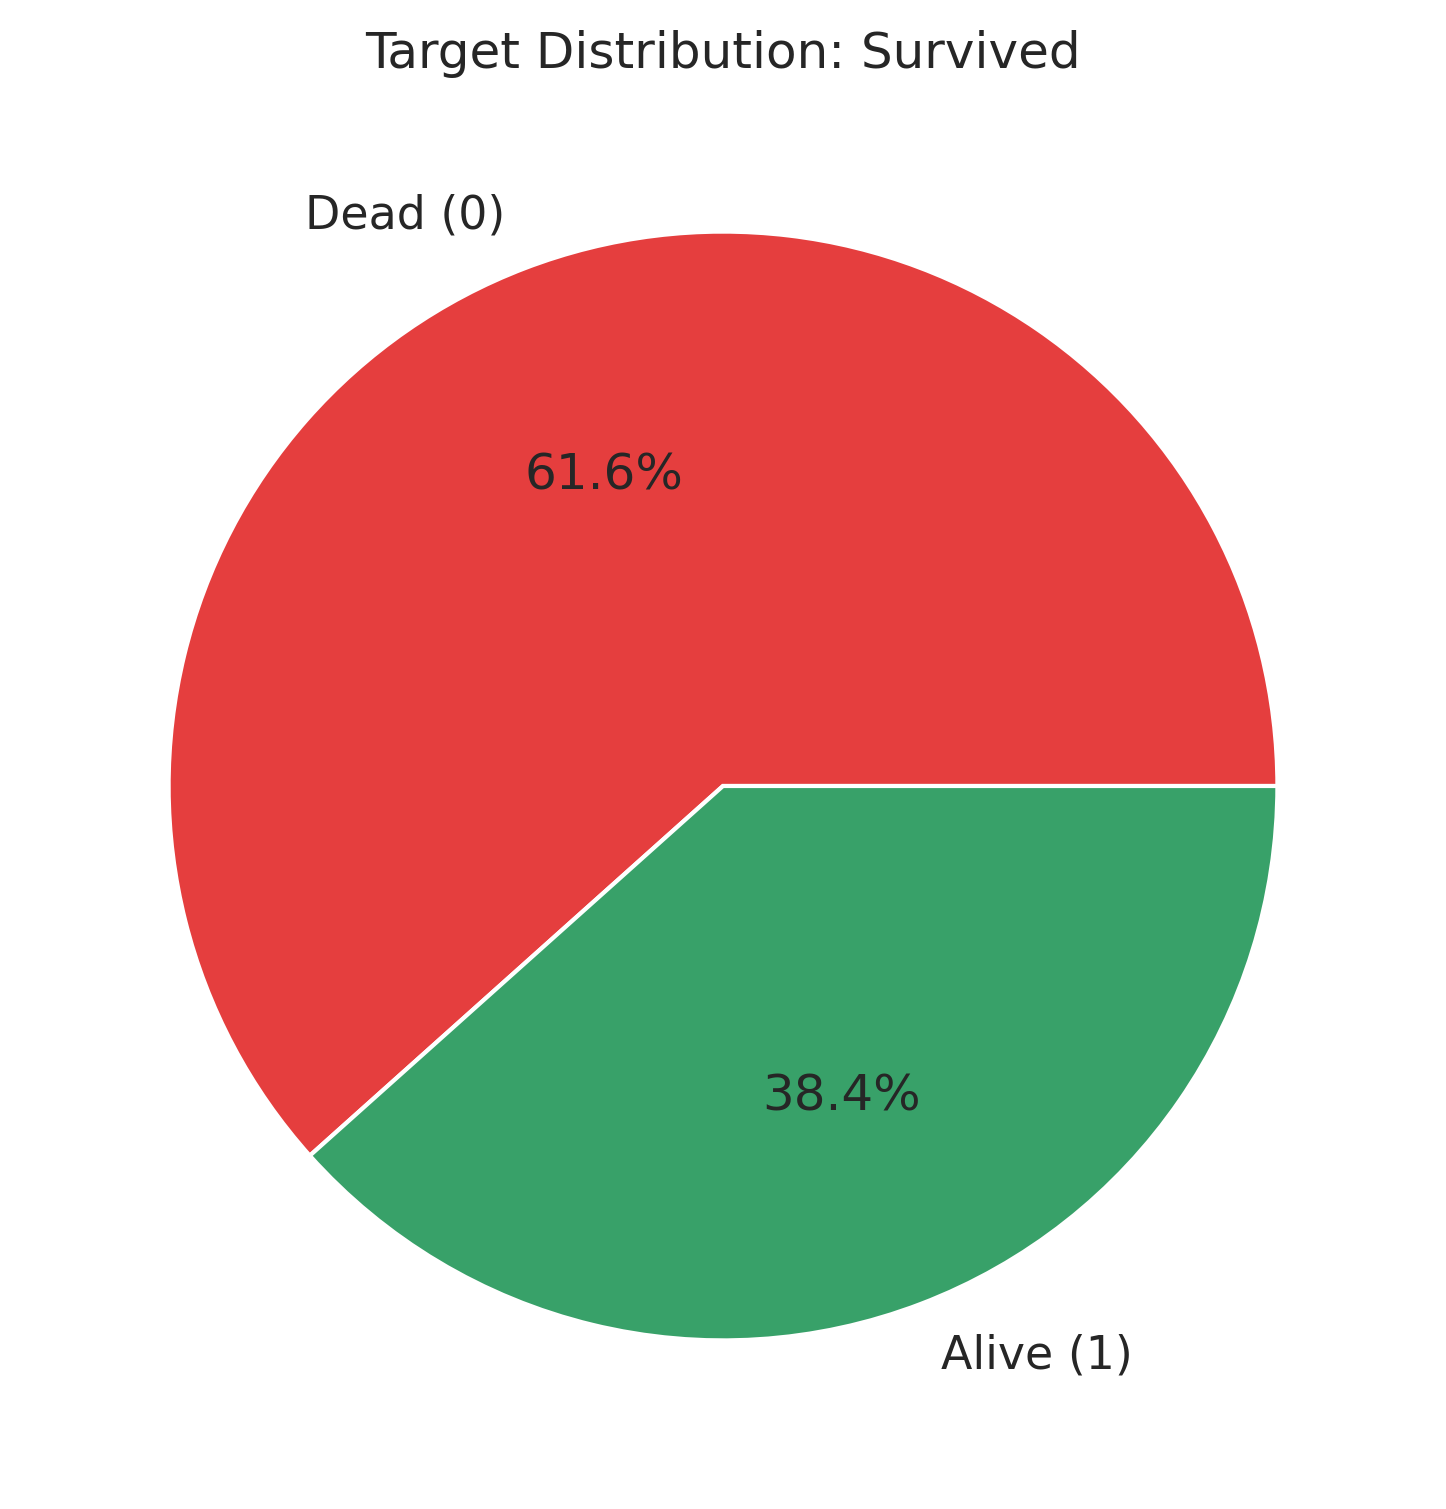
\includegraphics[width=0.60\textwidth]{images/target_dist.png}
    \caption{\textbf{Figure TAB-1} --- Target Distribution: Survived (1) vs.\ Not Survived (0). 38.4\% of passengers survived.
    \textit{Code:} \texttt{df['Survived'].value\_counts().plot(kind='bar')}.}
    \label{fig:tab_target}
\end{figure}

\subsection{Data Inspection and Missing Values}
Upon initial inspection, we identified the following distribution of missing values:
\begin{itemize}
    \item \textbf{Cabin:} 687 missing values (significant sparsity).
    \item \textbf{Age:} 177 missing values (requires imputation).
    \item \textbf{Embarked:} 2 missing values.
\end{itemize}

\subsection{Descriptive Statistics}

The numerical summary (\texttt{df.describe()}) reveals several notable properties of the dataset:

\begin{itemize}
    \item \textbf{Survival Rate:} Mean survival rate $\approx$ \textbf{38.4\%} --- a binary target with moderate class imbalance (38\% positive, 62\% negative).
    \item \textbf{Passenger Class:} Mean Pclass $= 2.31$, with the majority of passengers in 3rd class. Class 3 makes up $\sim$55\% of the passenger manifest.
    \item \textbf{Age:} Mean $= 29.7$ years, standard deviation $= 14.5$, range $= [0.42, 80]$. \textbf{177 values missing} (19.9\%) --- median imputation stratified by Pclass and Sex is recommended.
    \item \textbf{Fare:} Ranges from \$0 to \$512, with mean $= \$32.2$ and high std $= \$49.7$, indicating severe wealth disparity. Extreme outliers present.
    \item \textbf{SibSp / Parch:} Most passengers travelled alone (SibSp $= 0$: 68\%, Parch $= 0$: 76\%).
\end{itemize}

\begin{figure}[H]
    \centering
    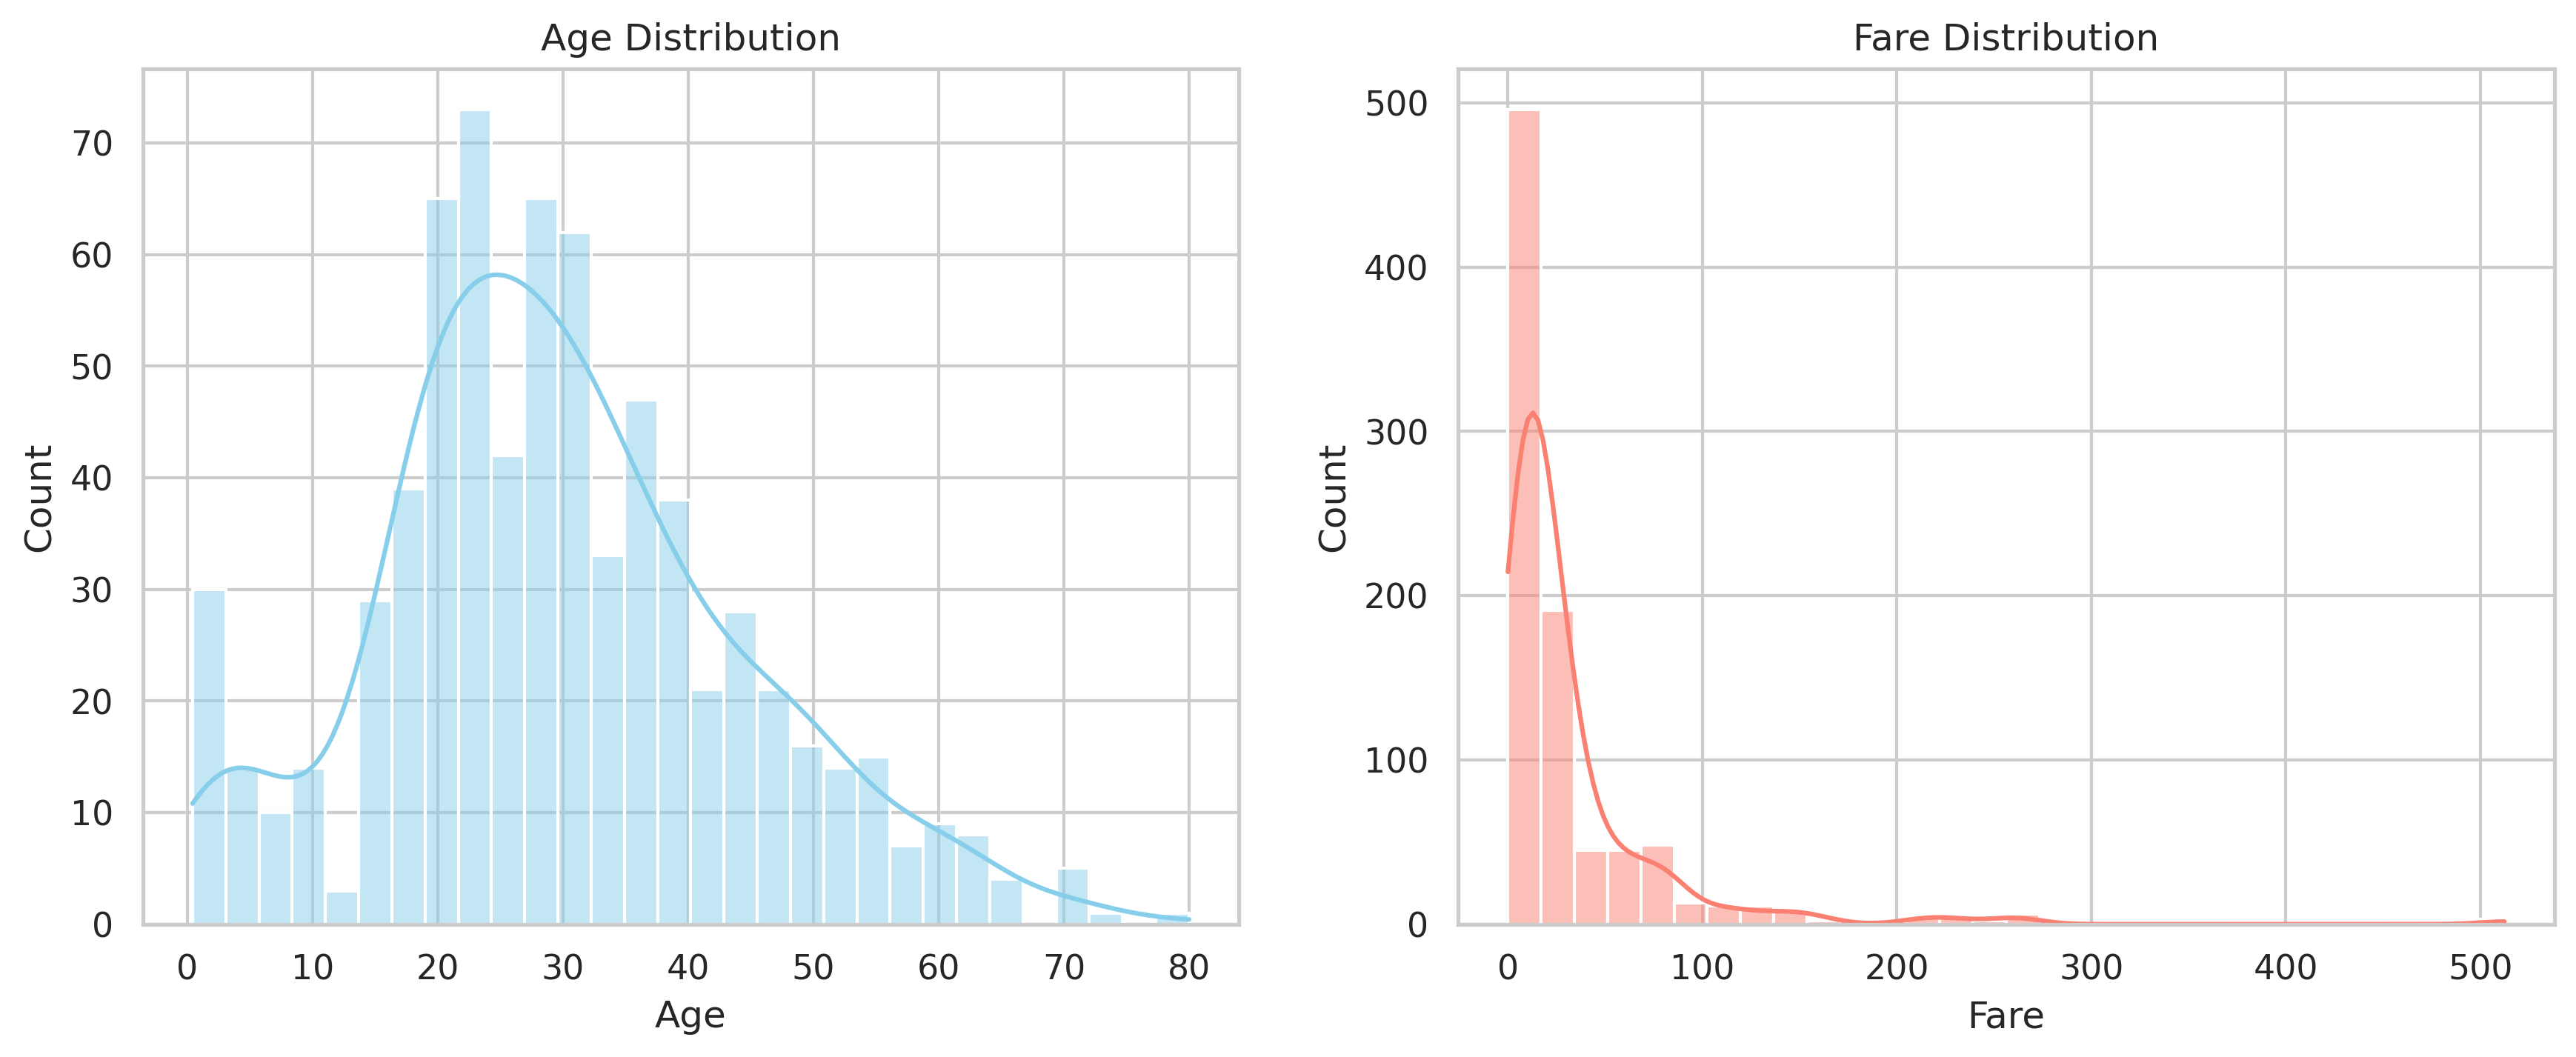
\includegraphics[width=0.90\textwidth]{images/age_fare_dist.png}
    \caption{\textbf{Figure TAB-2} --- Distribution of continuous features: Age (left) and Fare (right). Fare is strongly right-skewed; Age has a roughly normal distribution with a missing-data gap.
    \textit{Code:} \texttt{df[['Age','Fare']].hist(bins=30)}.}
    \label{fig:tab_num}
\end{figure}

\begin{figure}[H]
    \centering
    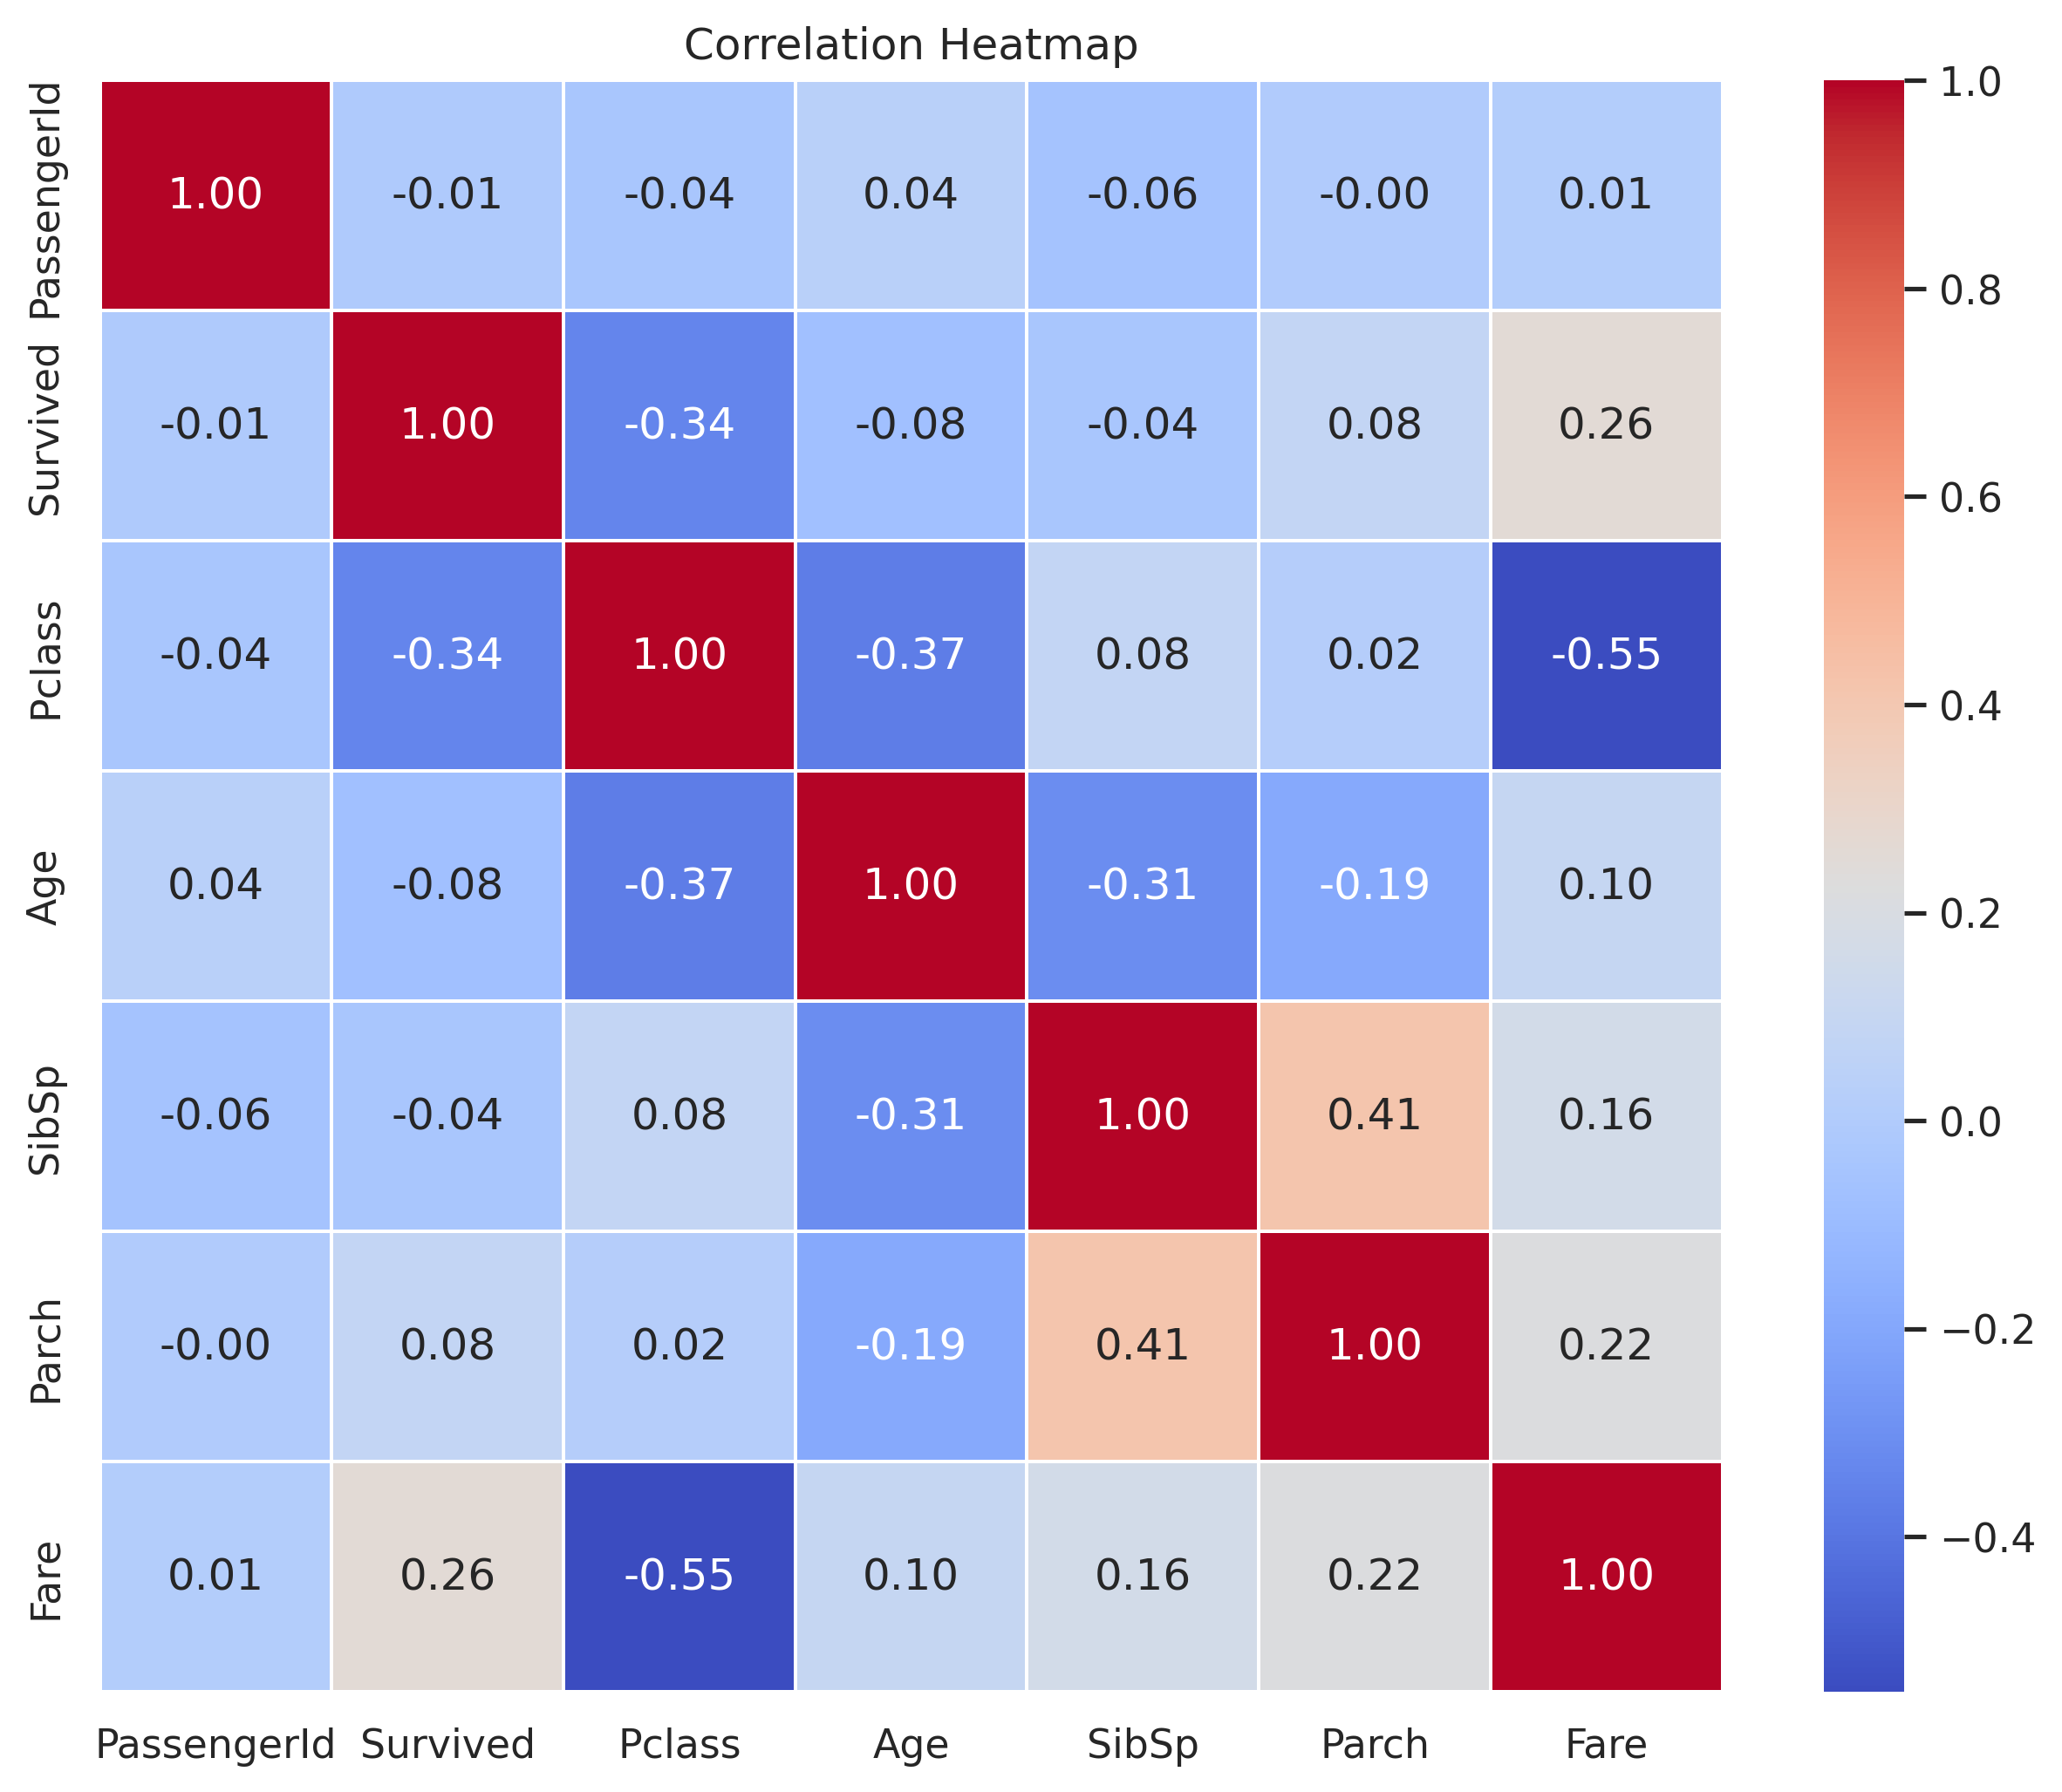
\includegraphics[width=0.70\textwidth]{images/heatmap.png}
    \caption{\textbf{Figure TAB-3} --- Pearson Correlation Matrix for numerical features. Key insight: Fare and Pclass are negatively correlated ($r \approx -0.55$); Survived correlates positively with Fare and negatively with Pclass.
    \textit{Code:} \texttt{sns.heatmap(df.corr(), annot=True)}.}
    \label{fig:tab_corr}
\end{figure}

\begin{figure}[H]
    \centering
    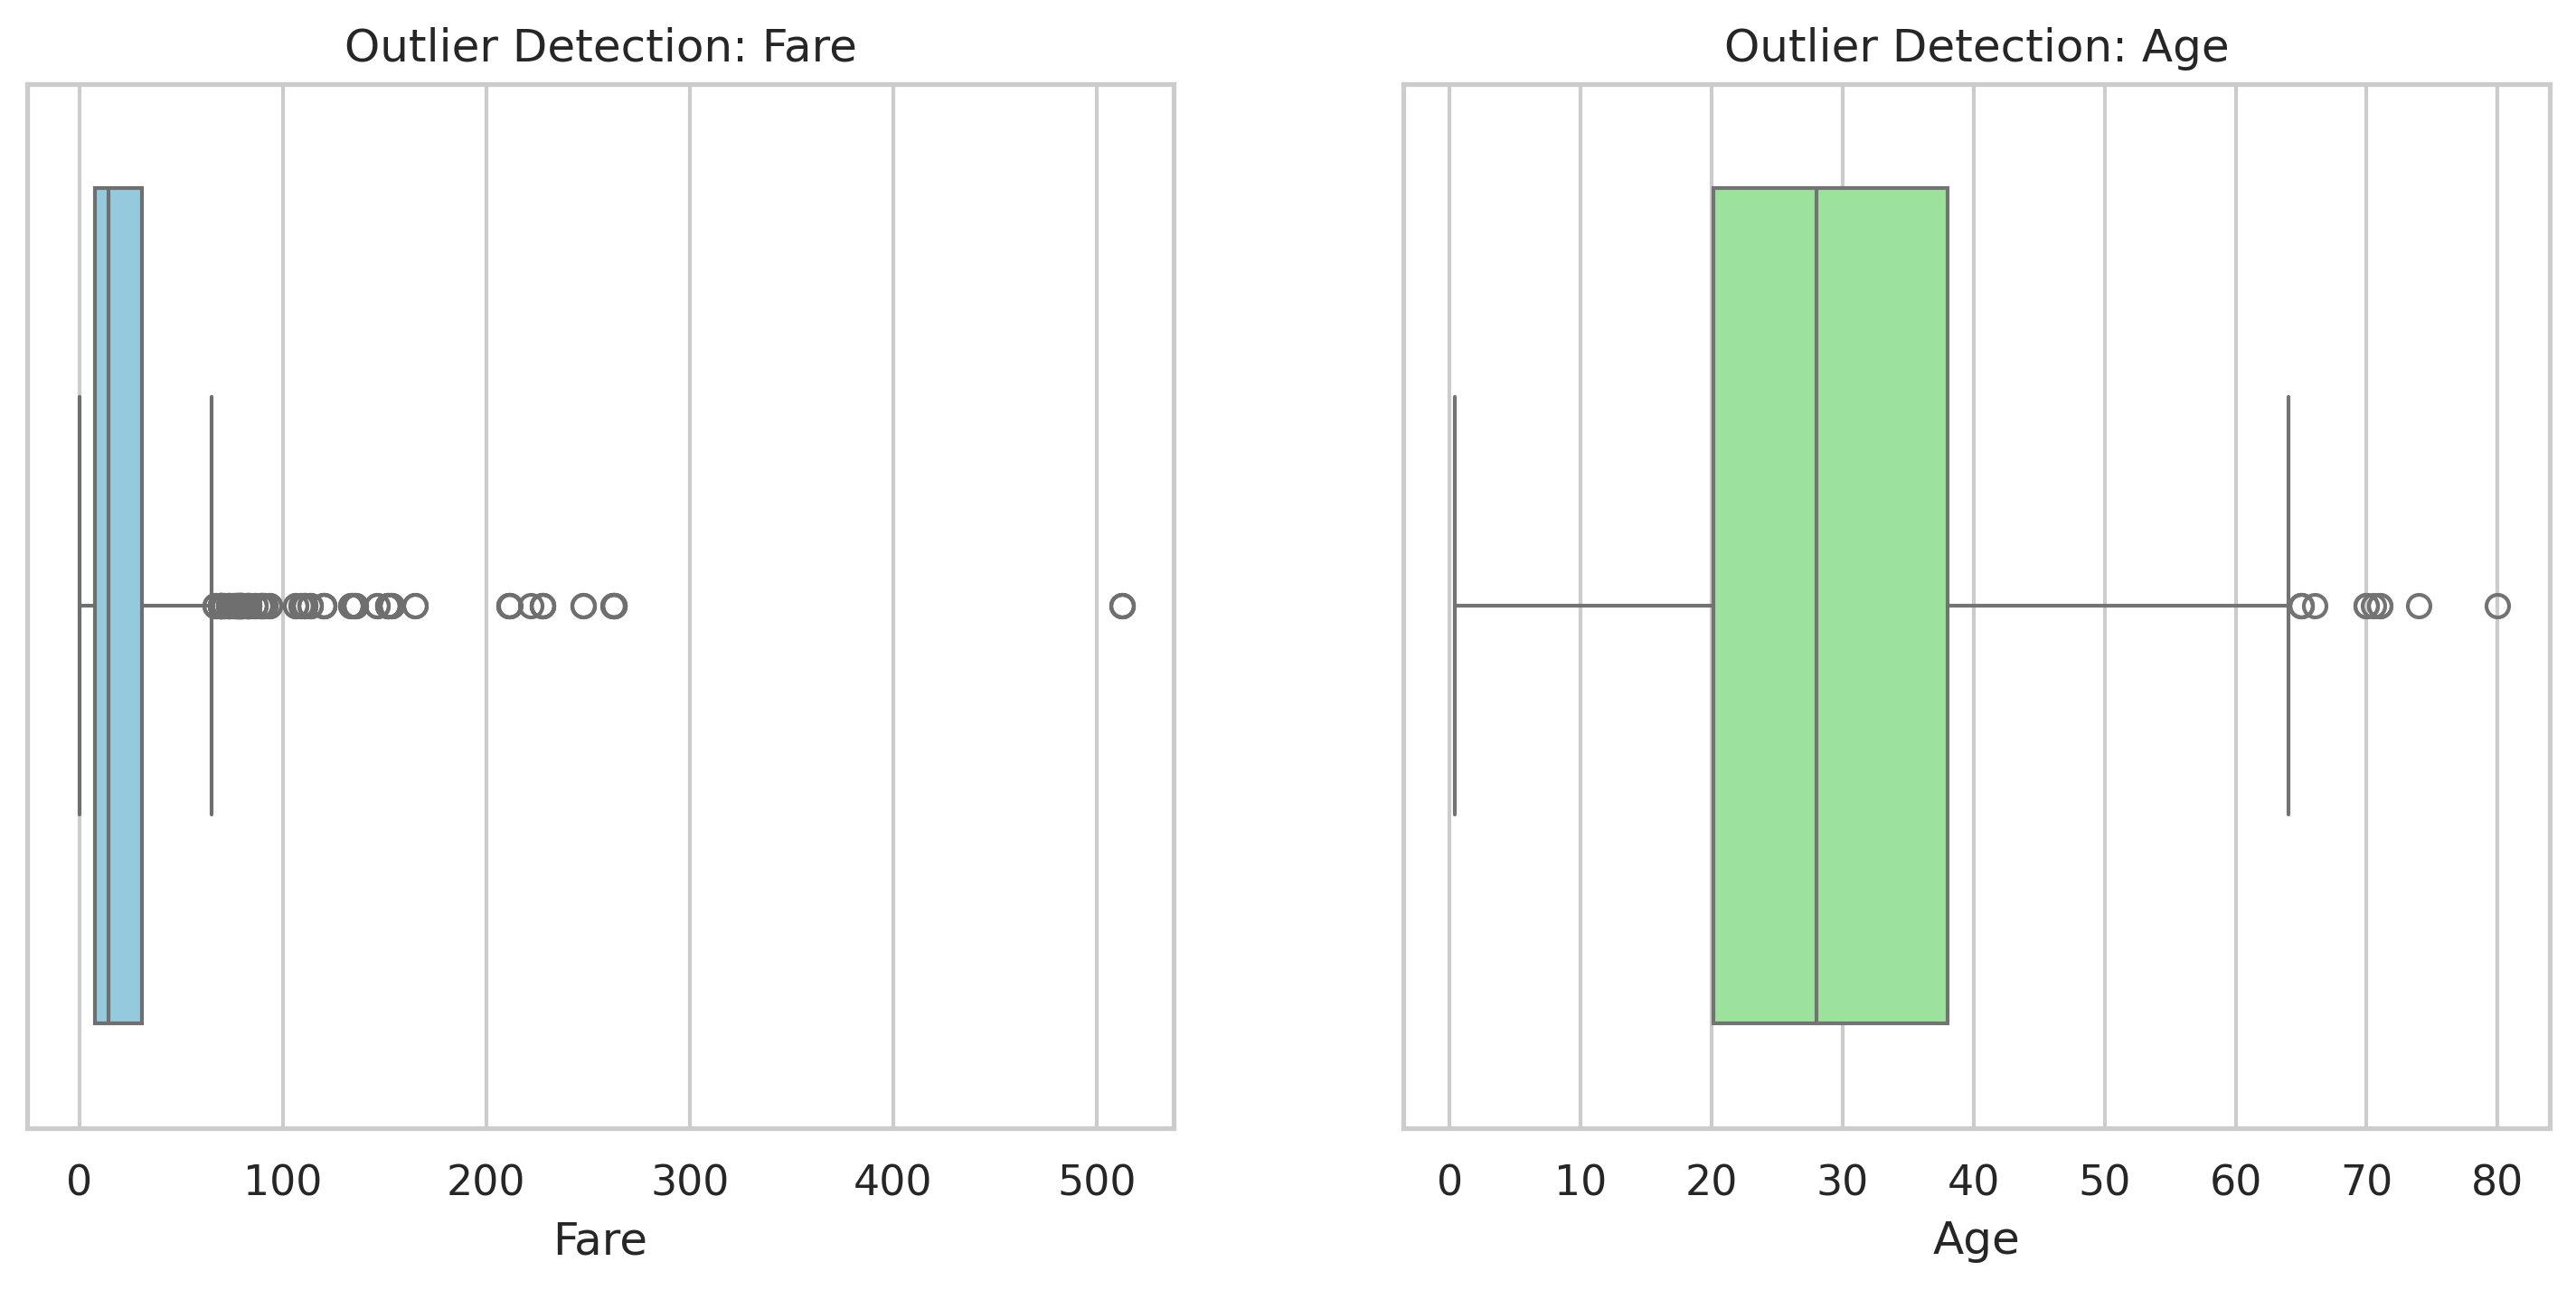
\includegraphics[width=0.90\textwidth]{images/outliers_boxplots.png}
    \caption{\textbf{Figure TAB-4} --- Outlier Detection via Boxplots for numerical features. Fare shows extreme upper outliers (max \$512); Age has mild outliers at both ends.
    \textit{Code:} \texttt{df.boxplot(column=['Age','Fare','SibSp','Parch'])}.}
    \label{fig:tab_outliers}
\end{figure}

\begin{figure}[H]
    \centering
    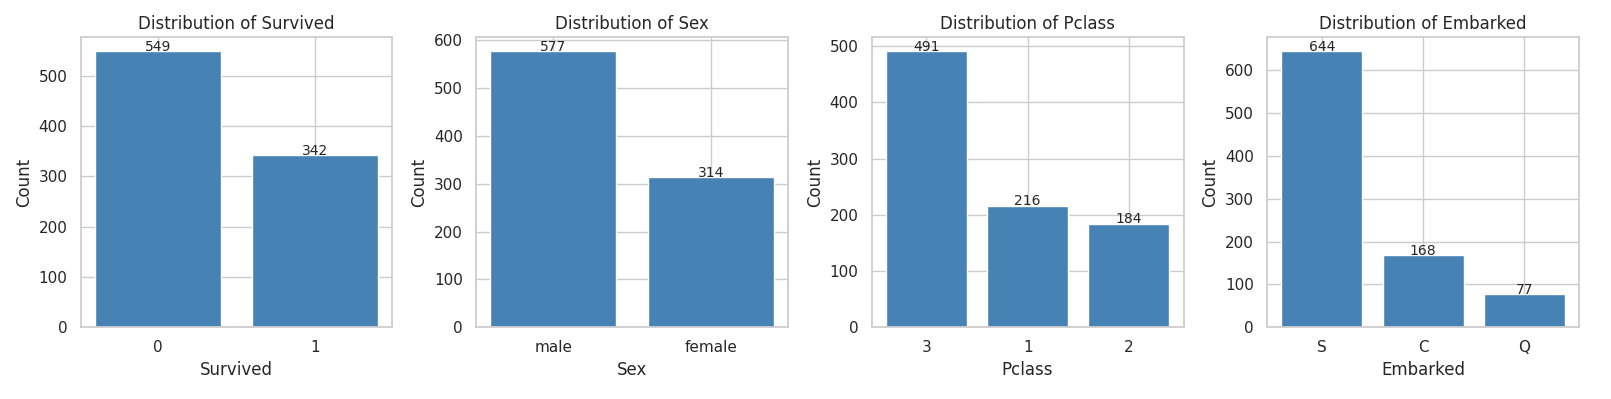
\includegraphics[width=0.95\textwidth]{images/tab_cat_dist.png}
    \caption{\textbf{Figure TAB-5} --- Distribution of Categorical Features: Sex, Pclass, and Embarked. Males and 3rd-class passengers dominate; Southampton (S) is the most common embarkation port.
    \textit{Code:} \texttt{df['Sex'].value\_counts().plot(kind='bar')} etc.}
    \label{fig:tab_cat}
\end{figure}

\begin{figure}[H]
    \centering
    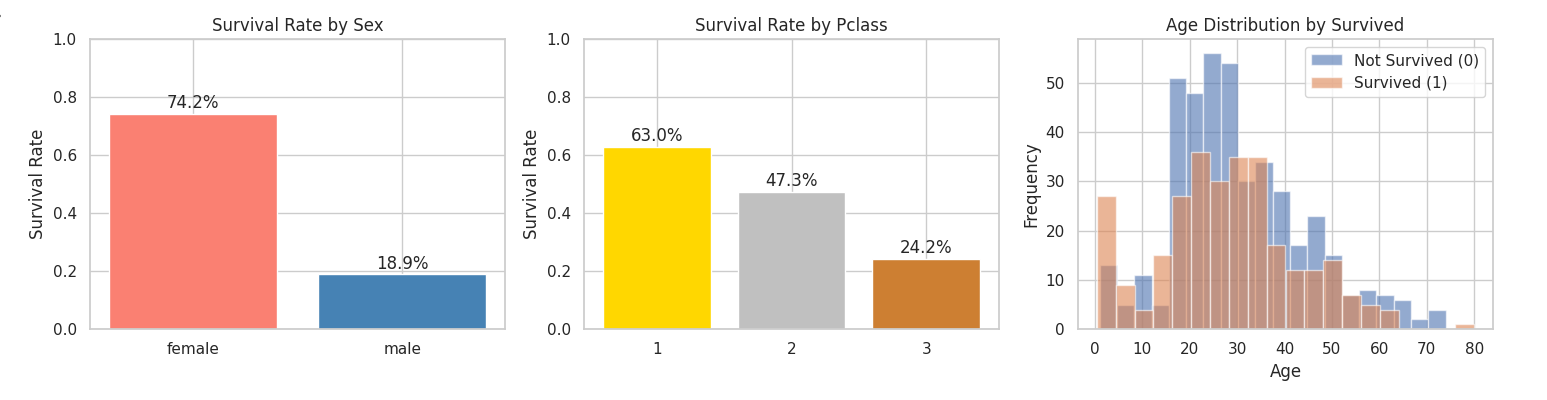
\includegraphics[width=0.95\textwidth]{images/tab_survival_groups.png}
    \caption{\textbf{Figure TAB-6} --- Survival Rate by Group (Sex, Pclass, Embarked). Females, 1st-class, and Cherbourg passengers show the highest survival rates.
    \textit{Code:} \texttt{df.groupby('Sex')['Survived'].mean().plot(kind='bar')} etc.}
    \label{fig:tab_surv_groups}
\end{figure}

\begin{figure}[H]
    \centering
    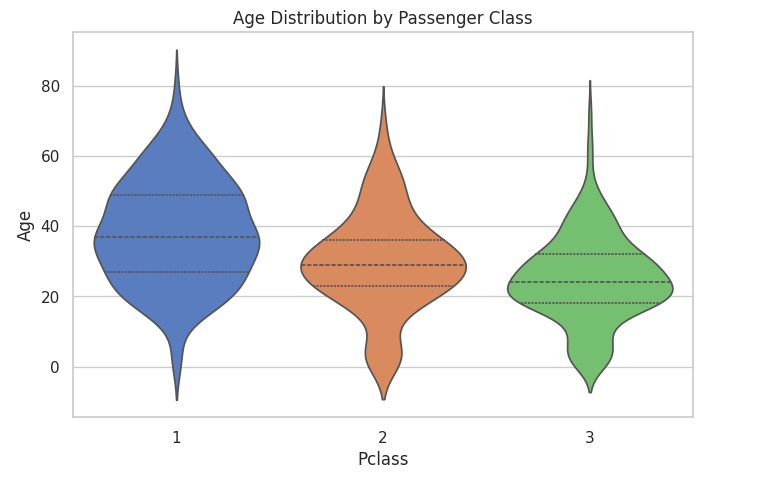
\includegraphics[width=0.60\textwidth]{images/tab_violin_age_pclass.png}
    \caption{\textbf{Figure TAB-7} --- Age Distribution by Passenger Class (violin plot). 1st-class passengers are older on average; 3rd class shows wider age spread including more children.
    \textit{Code:} \texttt{sns.violinplot(x='Pclass', y='Age', data=df)}.}
    \label{fig:tab_violin}
\end{figure}

\begin{figure}[H]
    \centering
    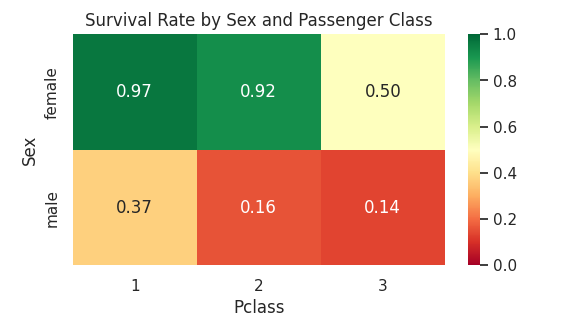
\includegraphics[width=0.55\textwidth]{images/tab_survival_heatmap.png}
    \caption{\textbf{Figure TAB-8} --- Survival Rate Heatmap by Sex and Passenger Class. The strongest interaction: 1st-class females had a $\sim$97\% survival rate vs.\ 3rd-class males at $\sim$14\%.
    \textit{Code:} \texttt{sns.heatmap(pivot\_table(Survived, Sex, Pclass))}.}
    \label{fig:tab_surv_heat}
\end{figure}

\subsection{Family Structure Analysis}

The \texttt{SibSp} (number of siblings/spouses) and \texttt{Parch} (number of parents/children) features jointly capture family structure on board, as shown in Figure TAB-9 below.

\begin{figure}[H]
    \centering
    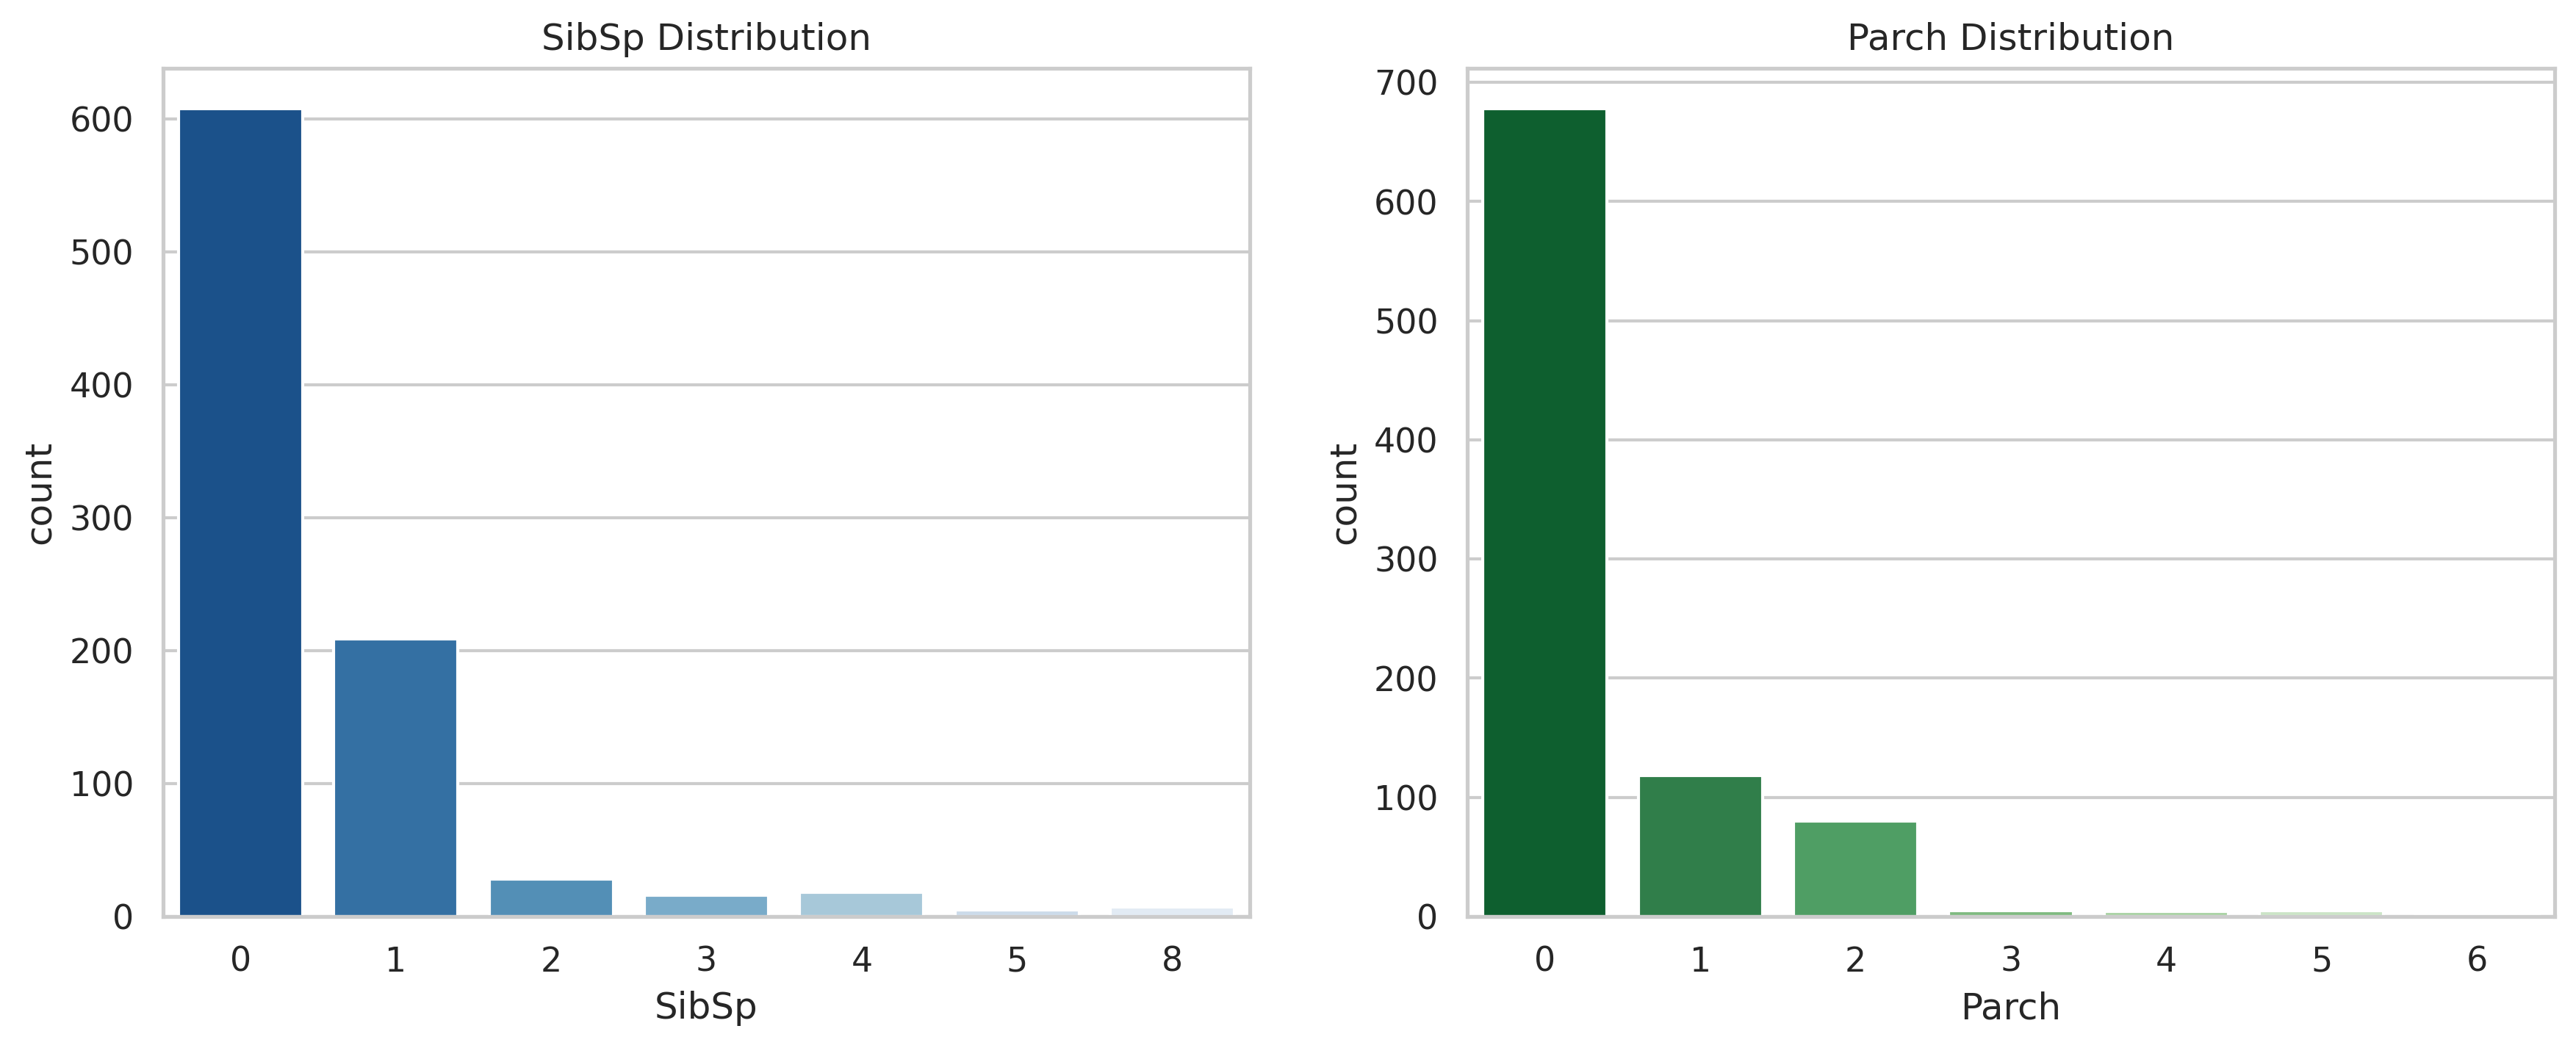
\includegraphics[width=0.90\textwidth]{images/sibsp_parch_dist.png}
    \caption{\textbf{Figure TAB-9} --- Distribution of \texttt{SibSp} (left) and \texttt{Parch} (right). The majority of passengers travelled without any family members aboard.
    \textit{Code:} \texttt{df['SibSp'].value\_counts().plot(kind='bar')} and \texttt{df['Parch'].value\_counts().plot(kind='bar')}.}
    \label{fig:tab_sibsp_parch}
\end{figure}

Key observations:
\begin{itemize}
    \item \textbf{Solo travellers dominate:} 68\% had SibSp $= 0$, and 76\% had Parch $= 0$.
    \item \textbf{Family size feature:} The derived feature \texttt{FamilySize = SibSp + Parch + 1} is commonly used in downstream modelling. Small families (2--4) tend to show higher survival rates than solo travellers or very large families (6+).
\end{itemize}

\subsection{Categorical Features vs.\ Survival Target}

Figure TAB-10 below directly compares survival rates across the three main categorical features, providing clear quantitative evidence of their predictive power.

\begin{figure}[H]
    \centering
    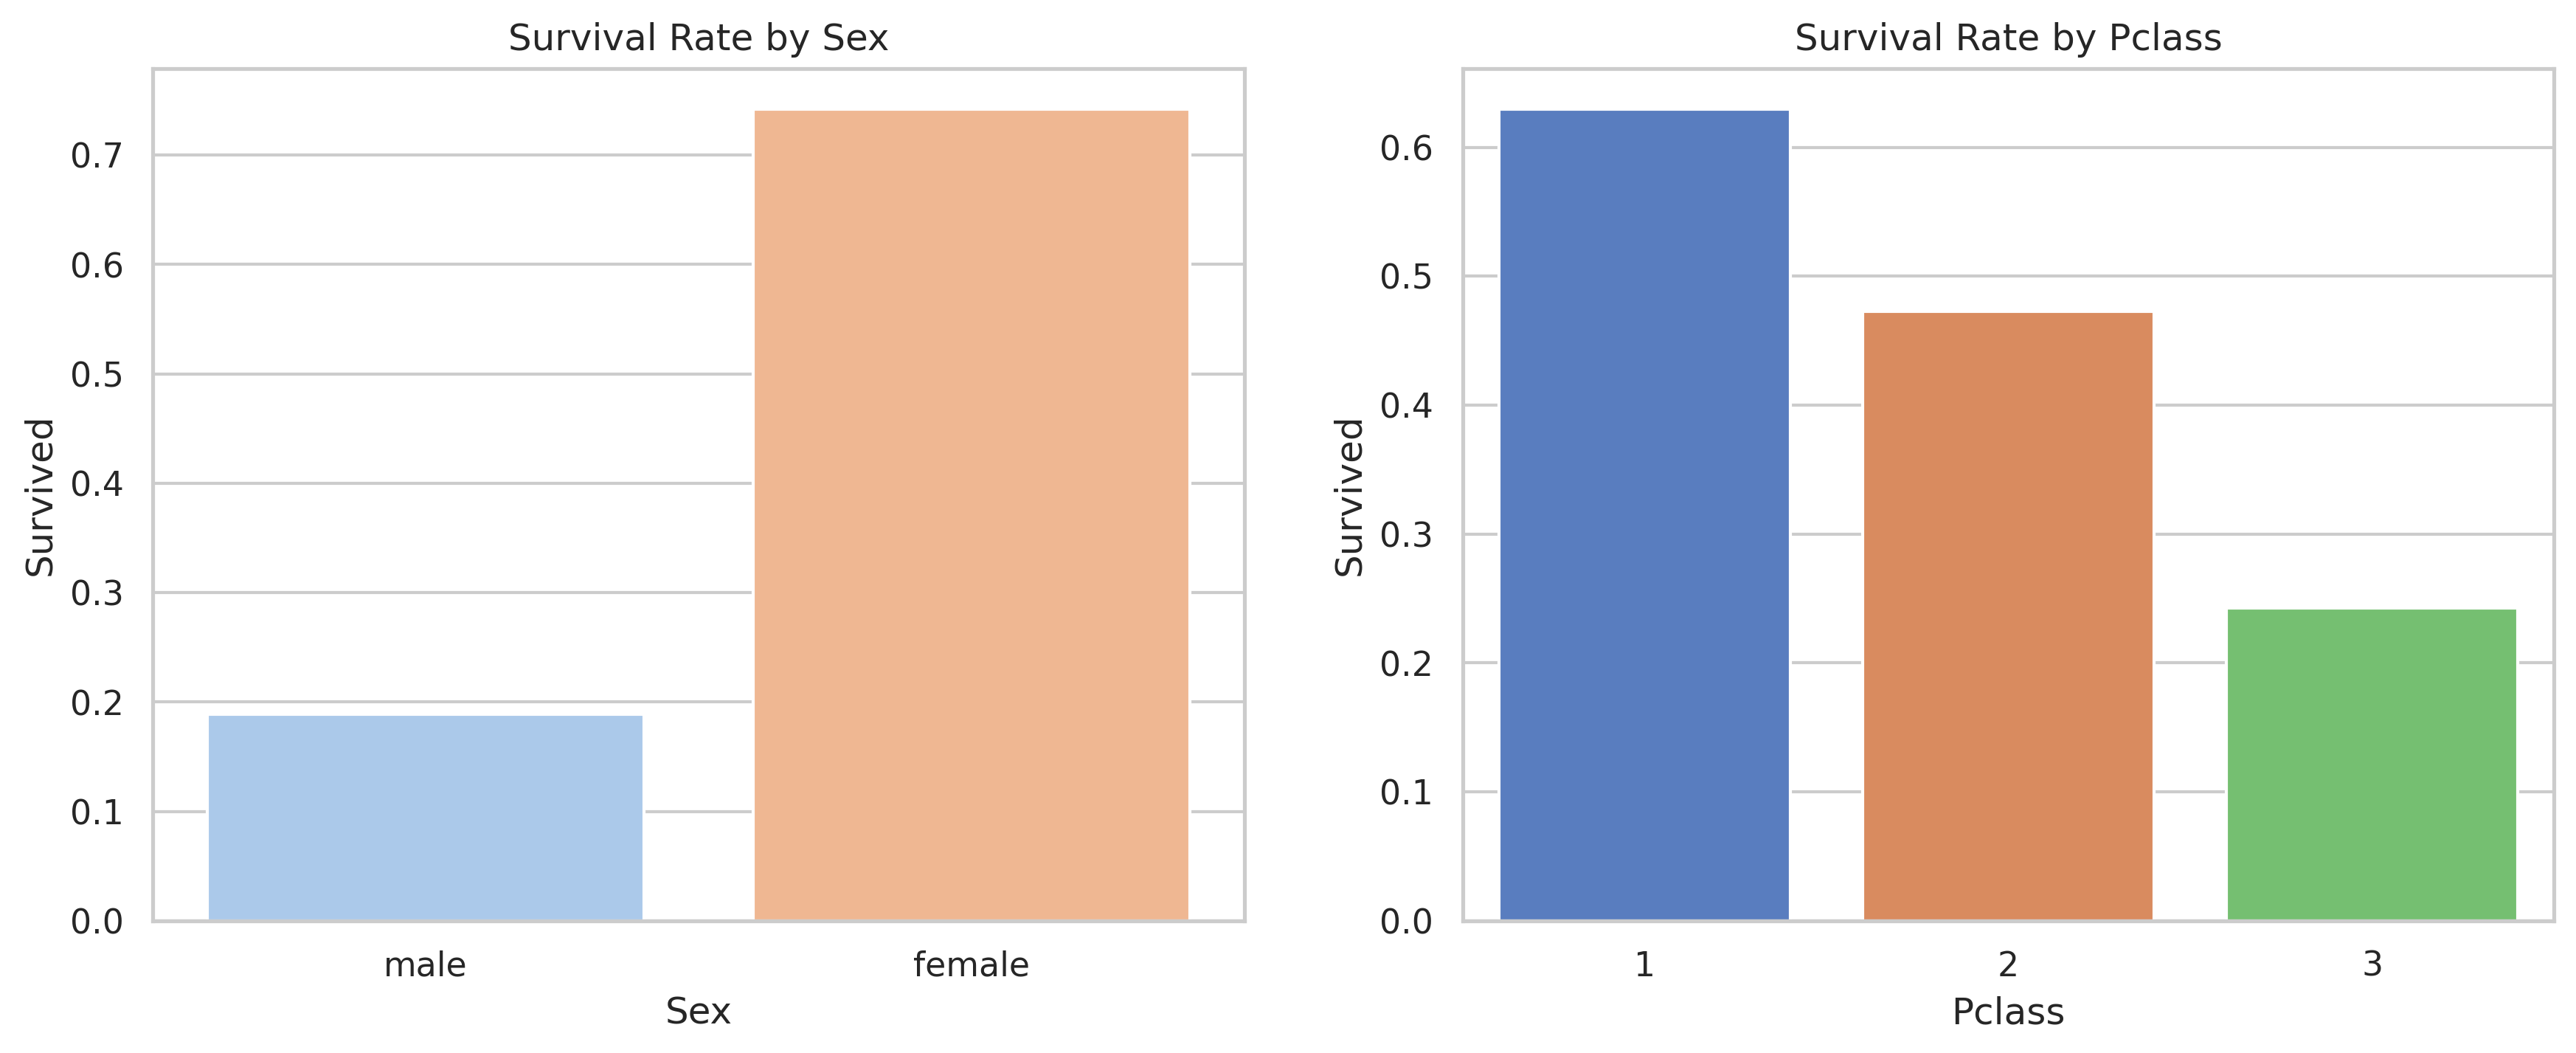
\includegraphics[width=0.90\textwidth]{images/cat_vs_target.png}
    \caption{\textbf{Figure TAB-10} --- Survival Rate by Categorical Feature Value. Each bar shows the proportion of passengers who survived within that category.
    \textit{Code:} \texttt{df.groupby('Sex')['Survived'].mean().plot(kind='bar')} etc.}
    \label{fig:tab_cat_vs_target}
\end{figure}

Key survival rates from the group analysis:
\begin{itemize}
    \item \textbf{Sex:} Female survival rate $\approx$ \textbf{74.2\%} vs.\ male $\approx$ \textbf{18.9\%} --- the strongest single predictor.
    \item \textbf{Passenger Class:} Pclass 1 $\approx$ \textbf{63\%}, Pclass 2 $\approx$ \textbf{47\%}, Pclass 3 $\approx$ \textbf{24\%} --- survival decreases monotonically with class number.
    \item \textbf{Embarked:} Cherbourg (C) shows slightly higher survival ($\sim$55\%) vs.\ Southampton (S) ($\sim$34\%), likely due to the higher proportion of 1st-class passengers boarding at Cherbourg.
\end{itemize}

\subsection{Ticket Prefix Analysis}

The \texttt{Ticket} column contains alphanumeric codes with varying prefixes that may encode booking class or origin information. The frequency distribution of ticket prefixes is shown in Figure TAB-11 below.

\begin{figure}[H]
    \centering
    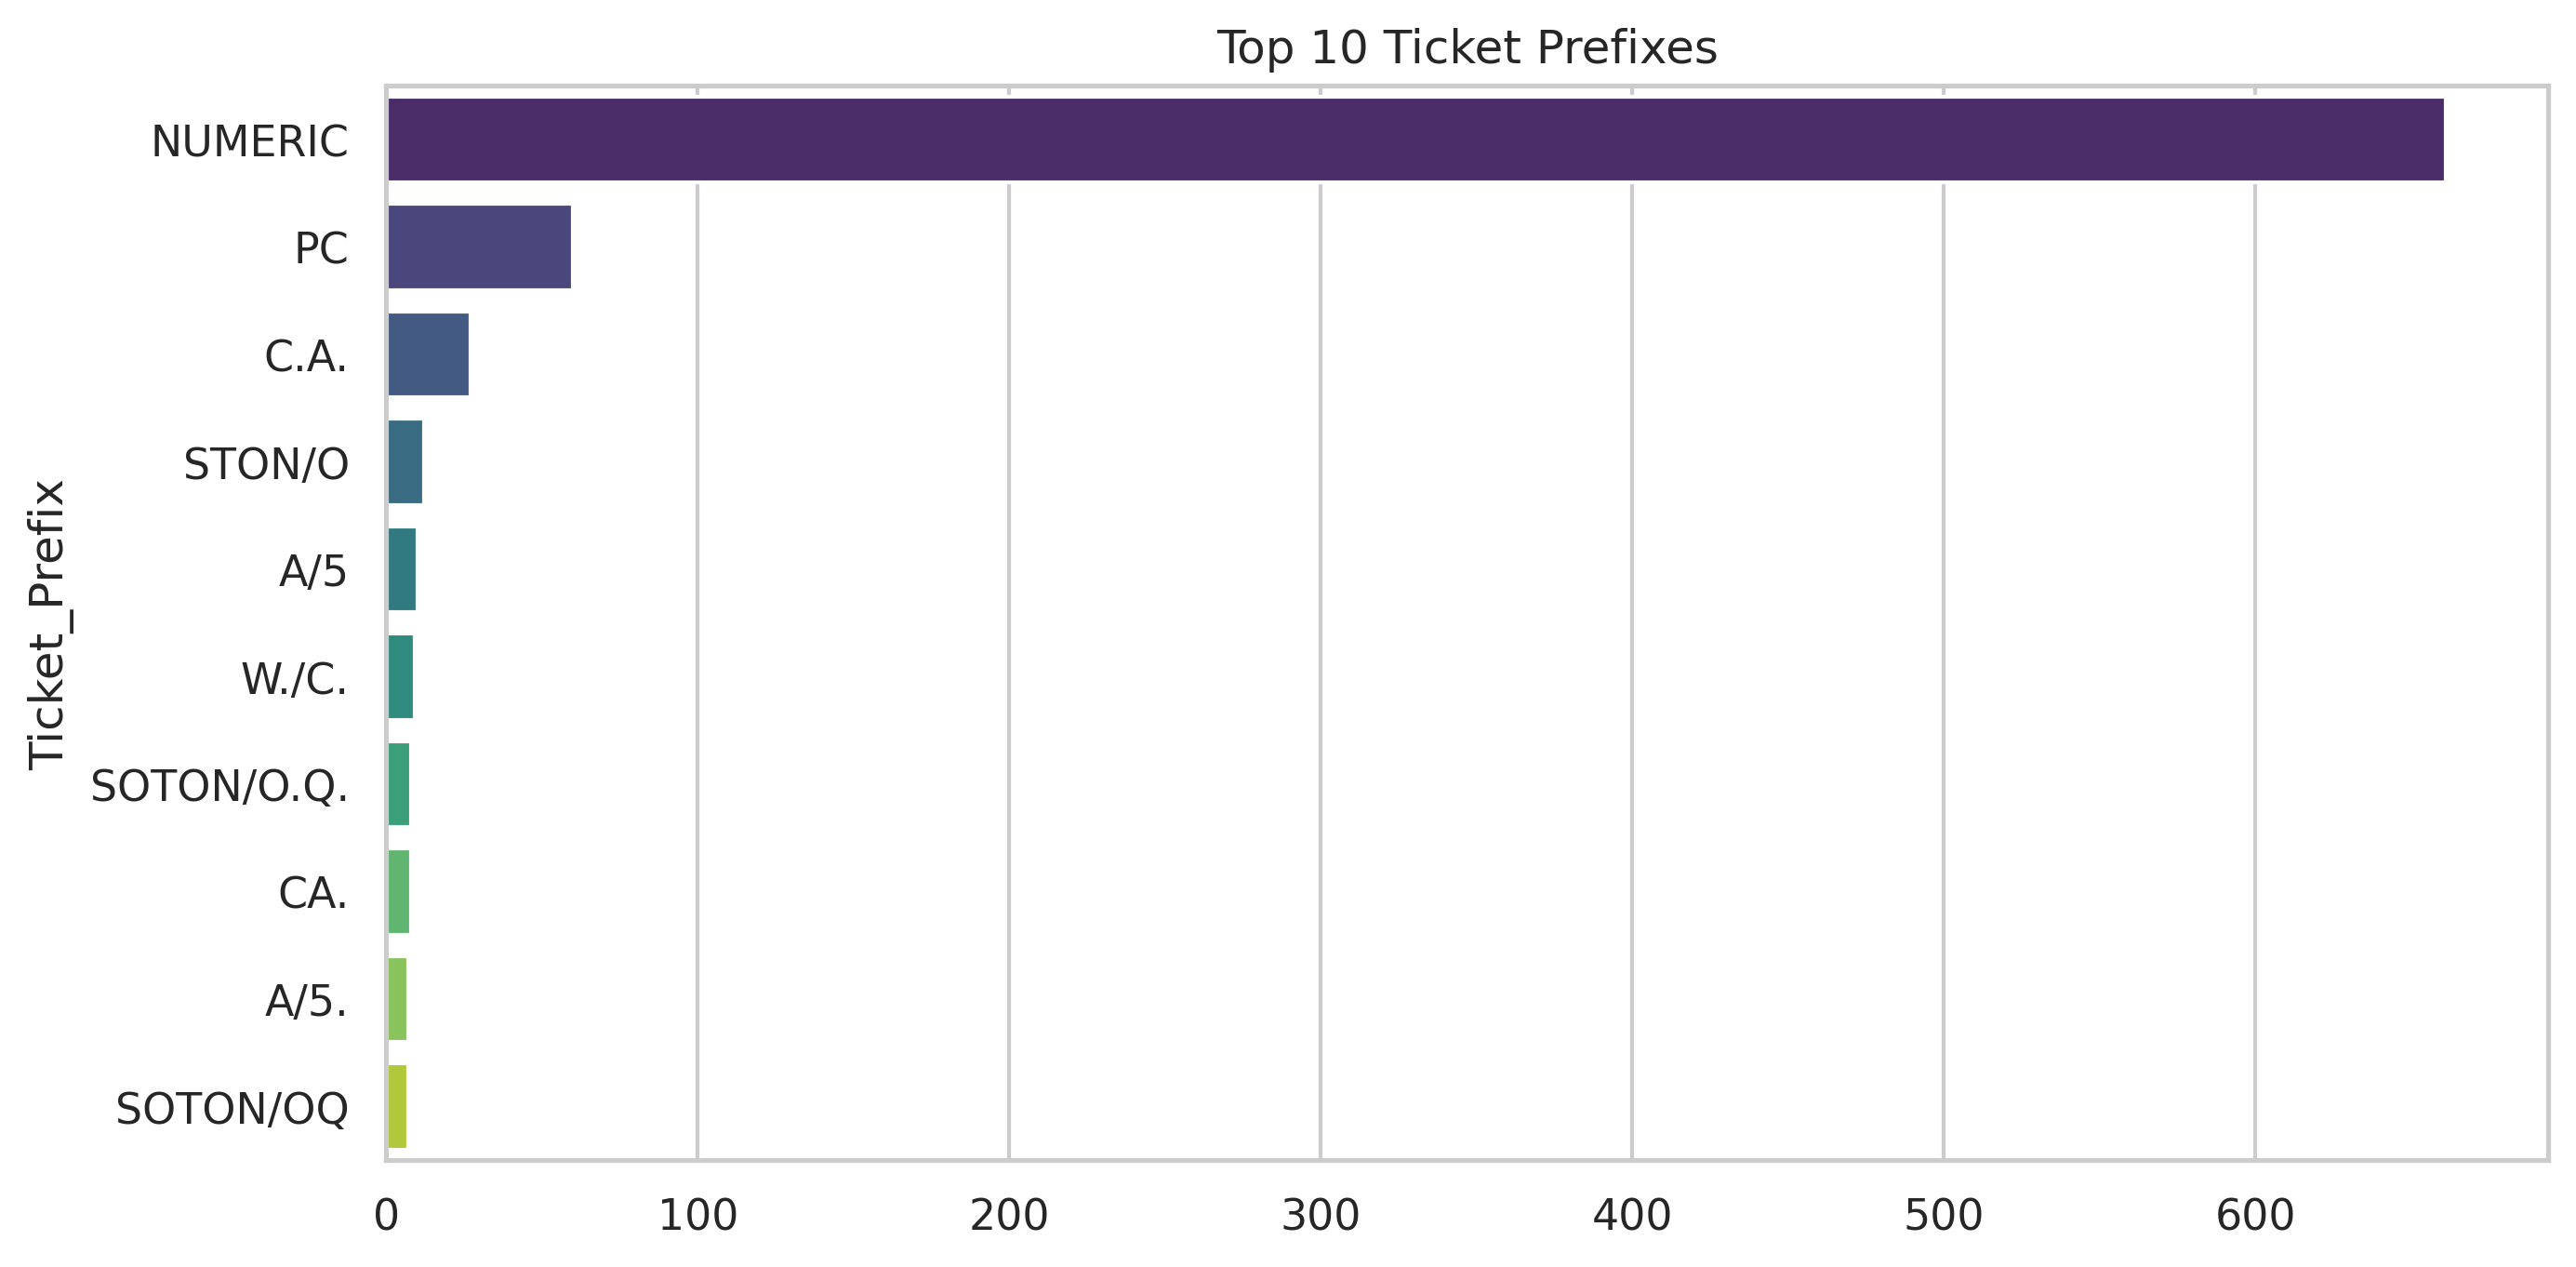
\includegraphics[width=0.85\textwidth]{images/ticket_prefix.png}
    \caption{\textbf{Figure TAB-11} --- Ticket Prefix Distribution. Numeric-only tickets dominate; named prefixes (e.g., ``PC'', ``SOTON'', ``CA'') may encode origin or class information.
    \textit{Code:} \texttt{df['Ticket'].str.extract(r'\^([A-Za-z./]+)')} then \texttt{value\_counts()}.}
    \label{fig:tab_ticket}
\end{figure}

\begin{itemize}
    \item Numeric-only tickets (no prefix) constitute the largest group, likely corresponding to 3rd-class passengers.
    \item Prefix \texttt{PC} (Paris Cherbourg) is associated with high-fare 1st-class passengers.
    \item The \texttt{Ticket} feature is generally dropped or encoded as a binary ``has prefix / no prefix'' indicator for modelling.
\end{itemize}

\subsection{Key Findings and Preprocessing Recommendations}

\begin{importantbox}
\textbf{Summary of Tabular EDA Key Findings:}
\begin{itemize}
    \item \textbf{Gender is the dominant predictor:} Female survival ($\sim$74\%) is nearly \textbf{4$\times$} that of males ($\sim$19\%), consistent with the historical ``women and children first'' evacuation policy.
    \item \textbf{Class reflects socioeconomic advantage:} 1st-class passengers ($\sim$63\% survived) had better access to lifeboats. The Fare--Pclass correlation ($r \approx -0.55$) confirms that higher fares correspond to lower (better) class numbers.
    \item \textbf{Age matters at the extremes:} Children (Age $<$ 10) show higher survival; elderly passengers (Age $>$ 60) show lower survival. The violin plot by Pclass confirms broader age variance in 3rd class.
    \item \textbf{Embarkation point is a proxy for class:} Cherbourg passengers show higher survival due to concentration of 1st-class travellers, not any causal embarkation effect.
    \item \textbf{Missing data plan:}
    \begin{itemize}
        \item \texttt{Cabin}: Drop or encode as binary (has cabin / no cabin). 77.1\% missing.
        \item \texttt{Age}: Impute with median stratified by Pclass and Sex. 19.9\% missing.
        \item \texttt{Embarked}: Impute with mode (``S''). Only 2 rows missing.
    \end{itemize}
    \item \textbf{Recommended preprocessing pipeline:}
    \begin{enumerate}
        \item Create \texttt{FamilySize = SibSp + Parch + 1} and \texttt{IsAlone} indicator.
        \item Extract title from \texttt{Name} (Mr., Mrs., Miss., Master.) as an ordinal feature.
        \item Encode \texttt{Sex} (0/1) and \texttt{Embarked} (one-hot).
        \item Normalise \texttt{Fare} (log-transform due to right skew).
        \item Drop \texttt{Cabin}, \texttt{Ticket}, \texttt{PassengerId}, \texttt{Name}.
    \end{enumerate}
\end{itemize}
\end{importantbox}

% =========================================================
% SECTION: TEXT DATA EDA
% =========================================================
\section{Exploratory Data Analysis: Text Data}
\label{sec:text}

\subsection{Dataset Overview}
For the text modality, we used the \textbf{SMS Spam Collection Dataset}, a well-known benchmark for binary text classification in natural language processing research. The dataset consists of English-language SMS messages labeled as either \texttt{ham} (legitimate personal messages) or \texttt{spam} (unsolicited promotional messages).

\begin{itemize}
    \item \textbf{Source:} \href{https://www.kaggle.com/datasets/marslinoedward/sms-spam-dataset/data}{SMS Spam Dataset --- Kaggle (marslinoedward)}
\end{itemize}

\begin{importantbox}
\textbf{Dataset Statistics:}
\begin{itemize}
    \item \textbf{Total Messages:} 5{,}572
    \item \textbf{Unique Messages:} 5{,}169 \hfill (403 exact duplicate rows detected)
    \item \textbf{Features:} 2 columns --- \texttt{label} (categorical: ham/spam) and \texttt{text} (raw string)
    \item \textbf{Ham (legitimate):} 4{,}825 messages \quad \textbf{86.6\%}
    \item \textbf{Spam:} 747 messages \quad \textbf{13.4\%}
    \item \textbf{Missing values:} 0 --- all rows are complete
\end{itemize}
\end{importantbox}

The class distribution is visualised in the figure below. The dataset contains approximately 6.5 ham messages for every 1 spam message --- a realistic ratio reflecting real-world SMS traffic, but one that has important implications for modelling: a naive majority-class classifier that always predicts ``ham'' achieves \textbf{86.6\% accuracy without learning anything}. Standard accuracy is therefore a misleading evaluation metric; F1-score (macro or weighted), Precision, Recall, and AUC-ROC are more appropriate.

\begin{figure}[H]
    \centering
    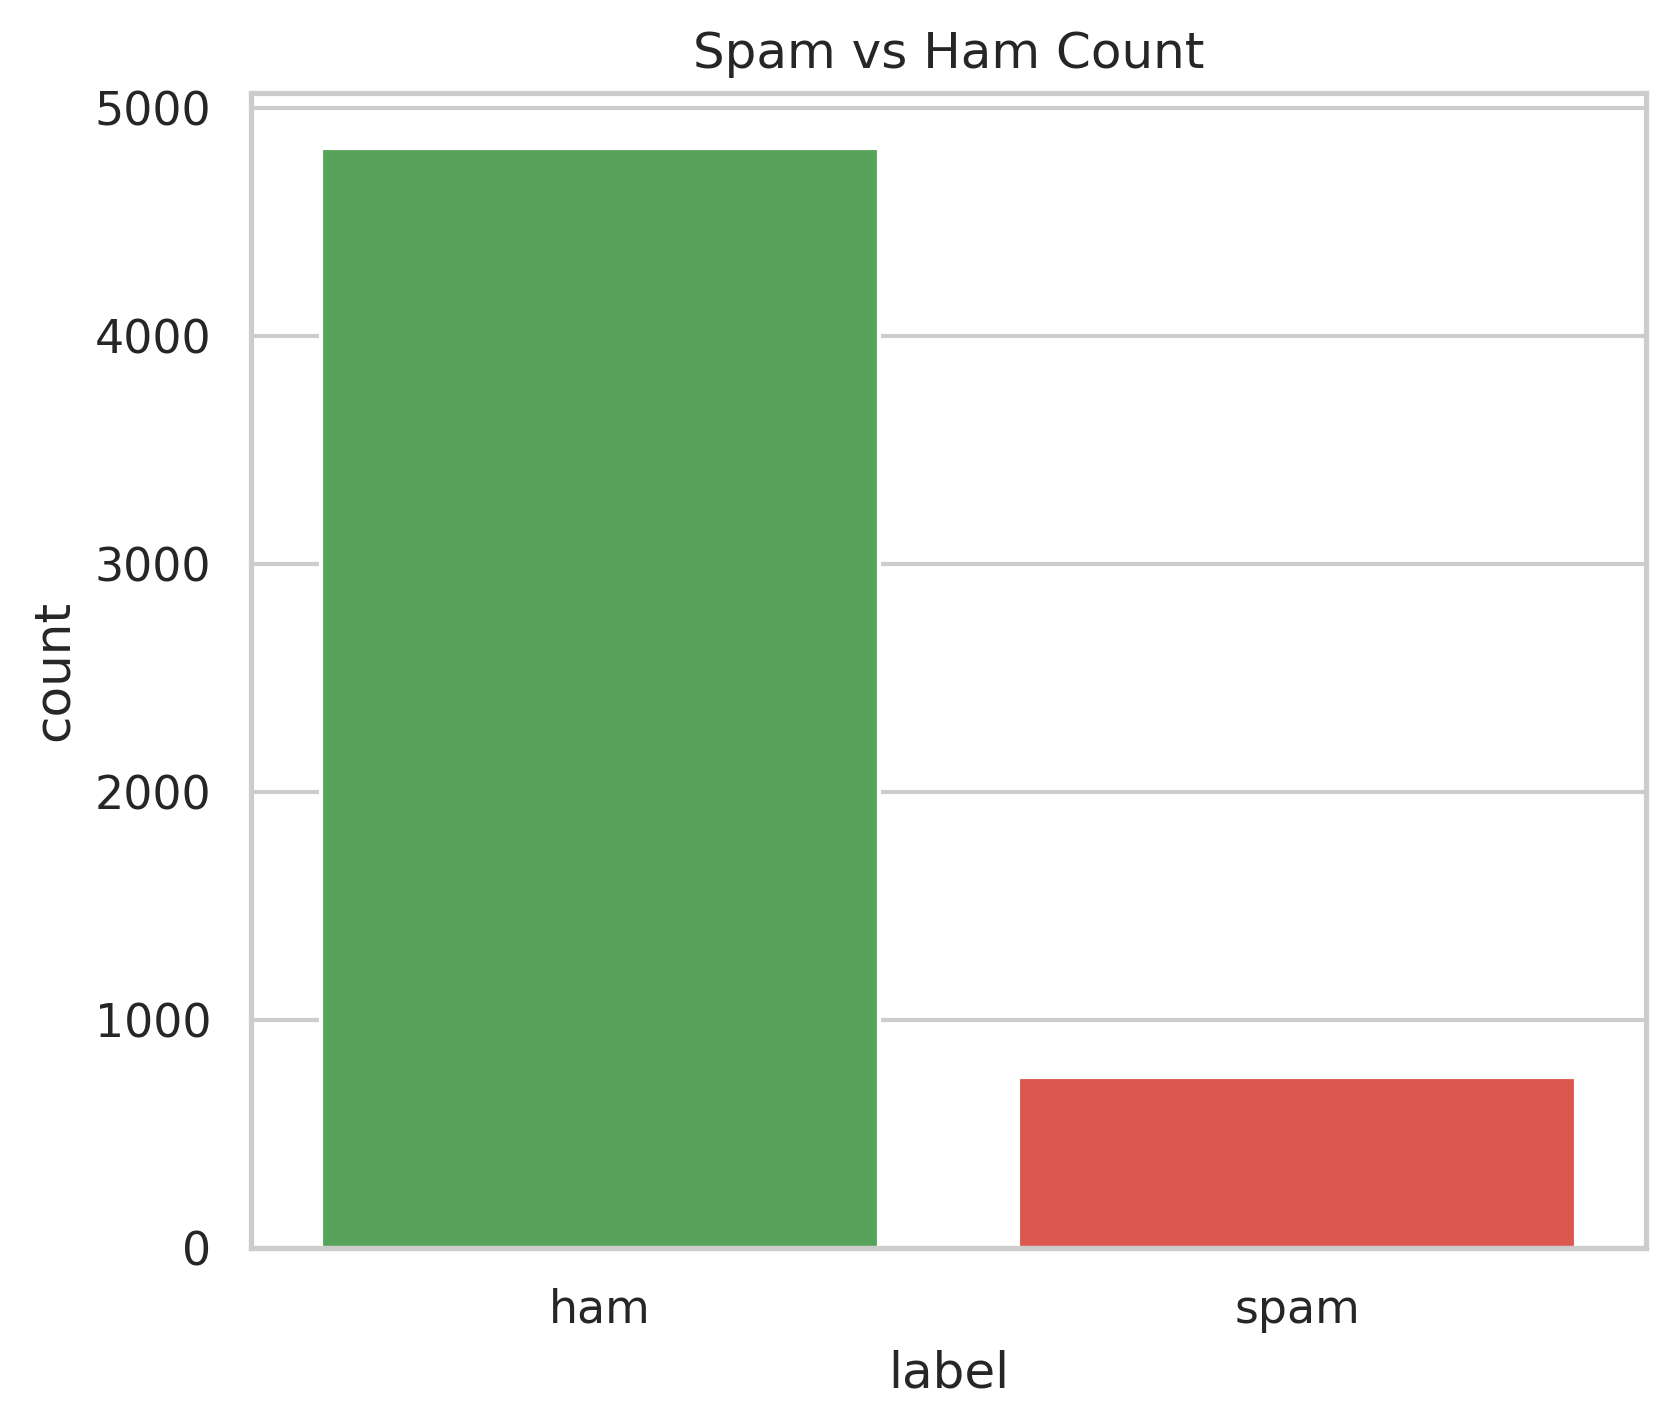
\includegraphics[width=0.60\textwidth]{images/text_target_dist.png}
    \caption{\textbf{Figure T1} --- Class Distribution: Ham vs.\ Spam (5{,}572 total messages; 86.6\%:13.4\%).
    \textit{Code:} \texttt{df\_text['label'].value\_counts().plot(kind='bar')}.}
    \label{fig:text_target}
\end{figure}

\subsection{Data Inspection and Quality}

\begin{itemize}
    \item \textbf{Shape:} \texttt{(5572, 2)} --- 5{,}572 rows, 2 columns (\texttt{label}, \texttt{text}).
    \item \textbf{Missing values:} None. Every row has both a label and a non-empty text field, making the dataset immediately usable without imputation.
    \item \textbf{Duplicate messages:} 403 exact duplicate rows detected (\texttt{df.duplicated().sum()}). These are predominantly very short, common ham phrases (``Ok'', ``I'll call you later'') that naturally recur across different conversation threads. While they do not represent data corruption, duplicates can introduce \emph{data leakage} if the same message appears in both train and test splits. \textbf{Deduplication is recommended} before any train/test split.
    \item \textbf{Label encoding:} \texttt{ham} $\rightarrow$ 0, \texttt{spam} $\rightarrow$ 1 for modelling.
\end{itemize}

\subsection{Message Length Analysis}

Message character length is one of the simplest yet most powerful raw features for separating ham from spam. Table T1 below summarises the statistics by label, and the resulting distributions are shown in Figure T2.

\begin{table}[H]
\centering
\caption{\textbf{Table T1} --- Message Length Statistics by Label (character count, including spaces)}
\label{tab:text_length}
\begin{tabular}{lrrrr}
\hline
\textbf{Label} & \textbf{Mean} & \textbf{Median} & \textbf{Min} & \textbf{Max} \\
\hline
Ham  & $\sim$71.5  & 52  & 2   & 910 \\
Spam & $\sim$138.7 & 149 & 13  & 224 \\
\hline
\end{tabular}
\end{table}

Key observations:
\begin{itemize}
    \item \textbf{Spam is nearly twice as long:} Mean spam length ($\sim$139 chars) is almost double that of ham ($\sim$72 chars). Spam authors pack promotional content, phone numbers, URLs, and urgency cues into each message.
    \item \textbf{Spam is length-bounded:} Maximum spam length (224 chars) is well below maximum ham length (910 chars), reflecting spammers' optimization for the 160-character SMS limit while legitimate messages can span multiple segments.
    \item \textbf{Low variance in spam:} Spam messages cluster tightly around the median (median $\approx$ mean $\approx$ 149 chars), indicating templated, length-optimised message structures.
    \item \textbf{High variance in ham:} Ham shows a long right tail (max = 910), ranging from single-word replies (``Ok'') to detailed multi-paragraph personal messages.
\end{itemize}

\begin{figure}[H]
    \centering
    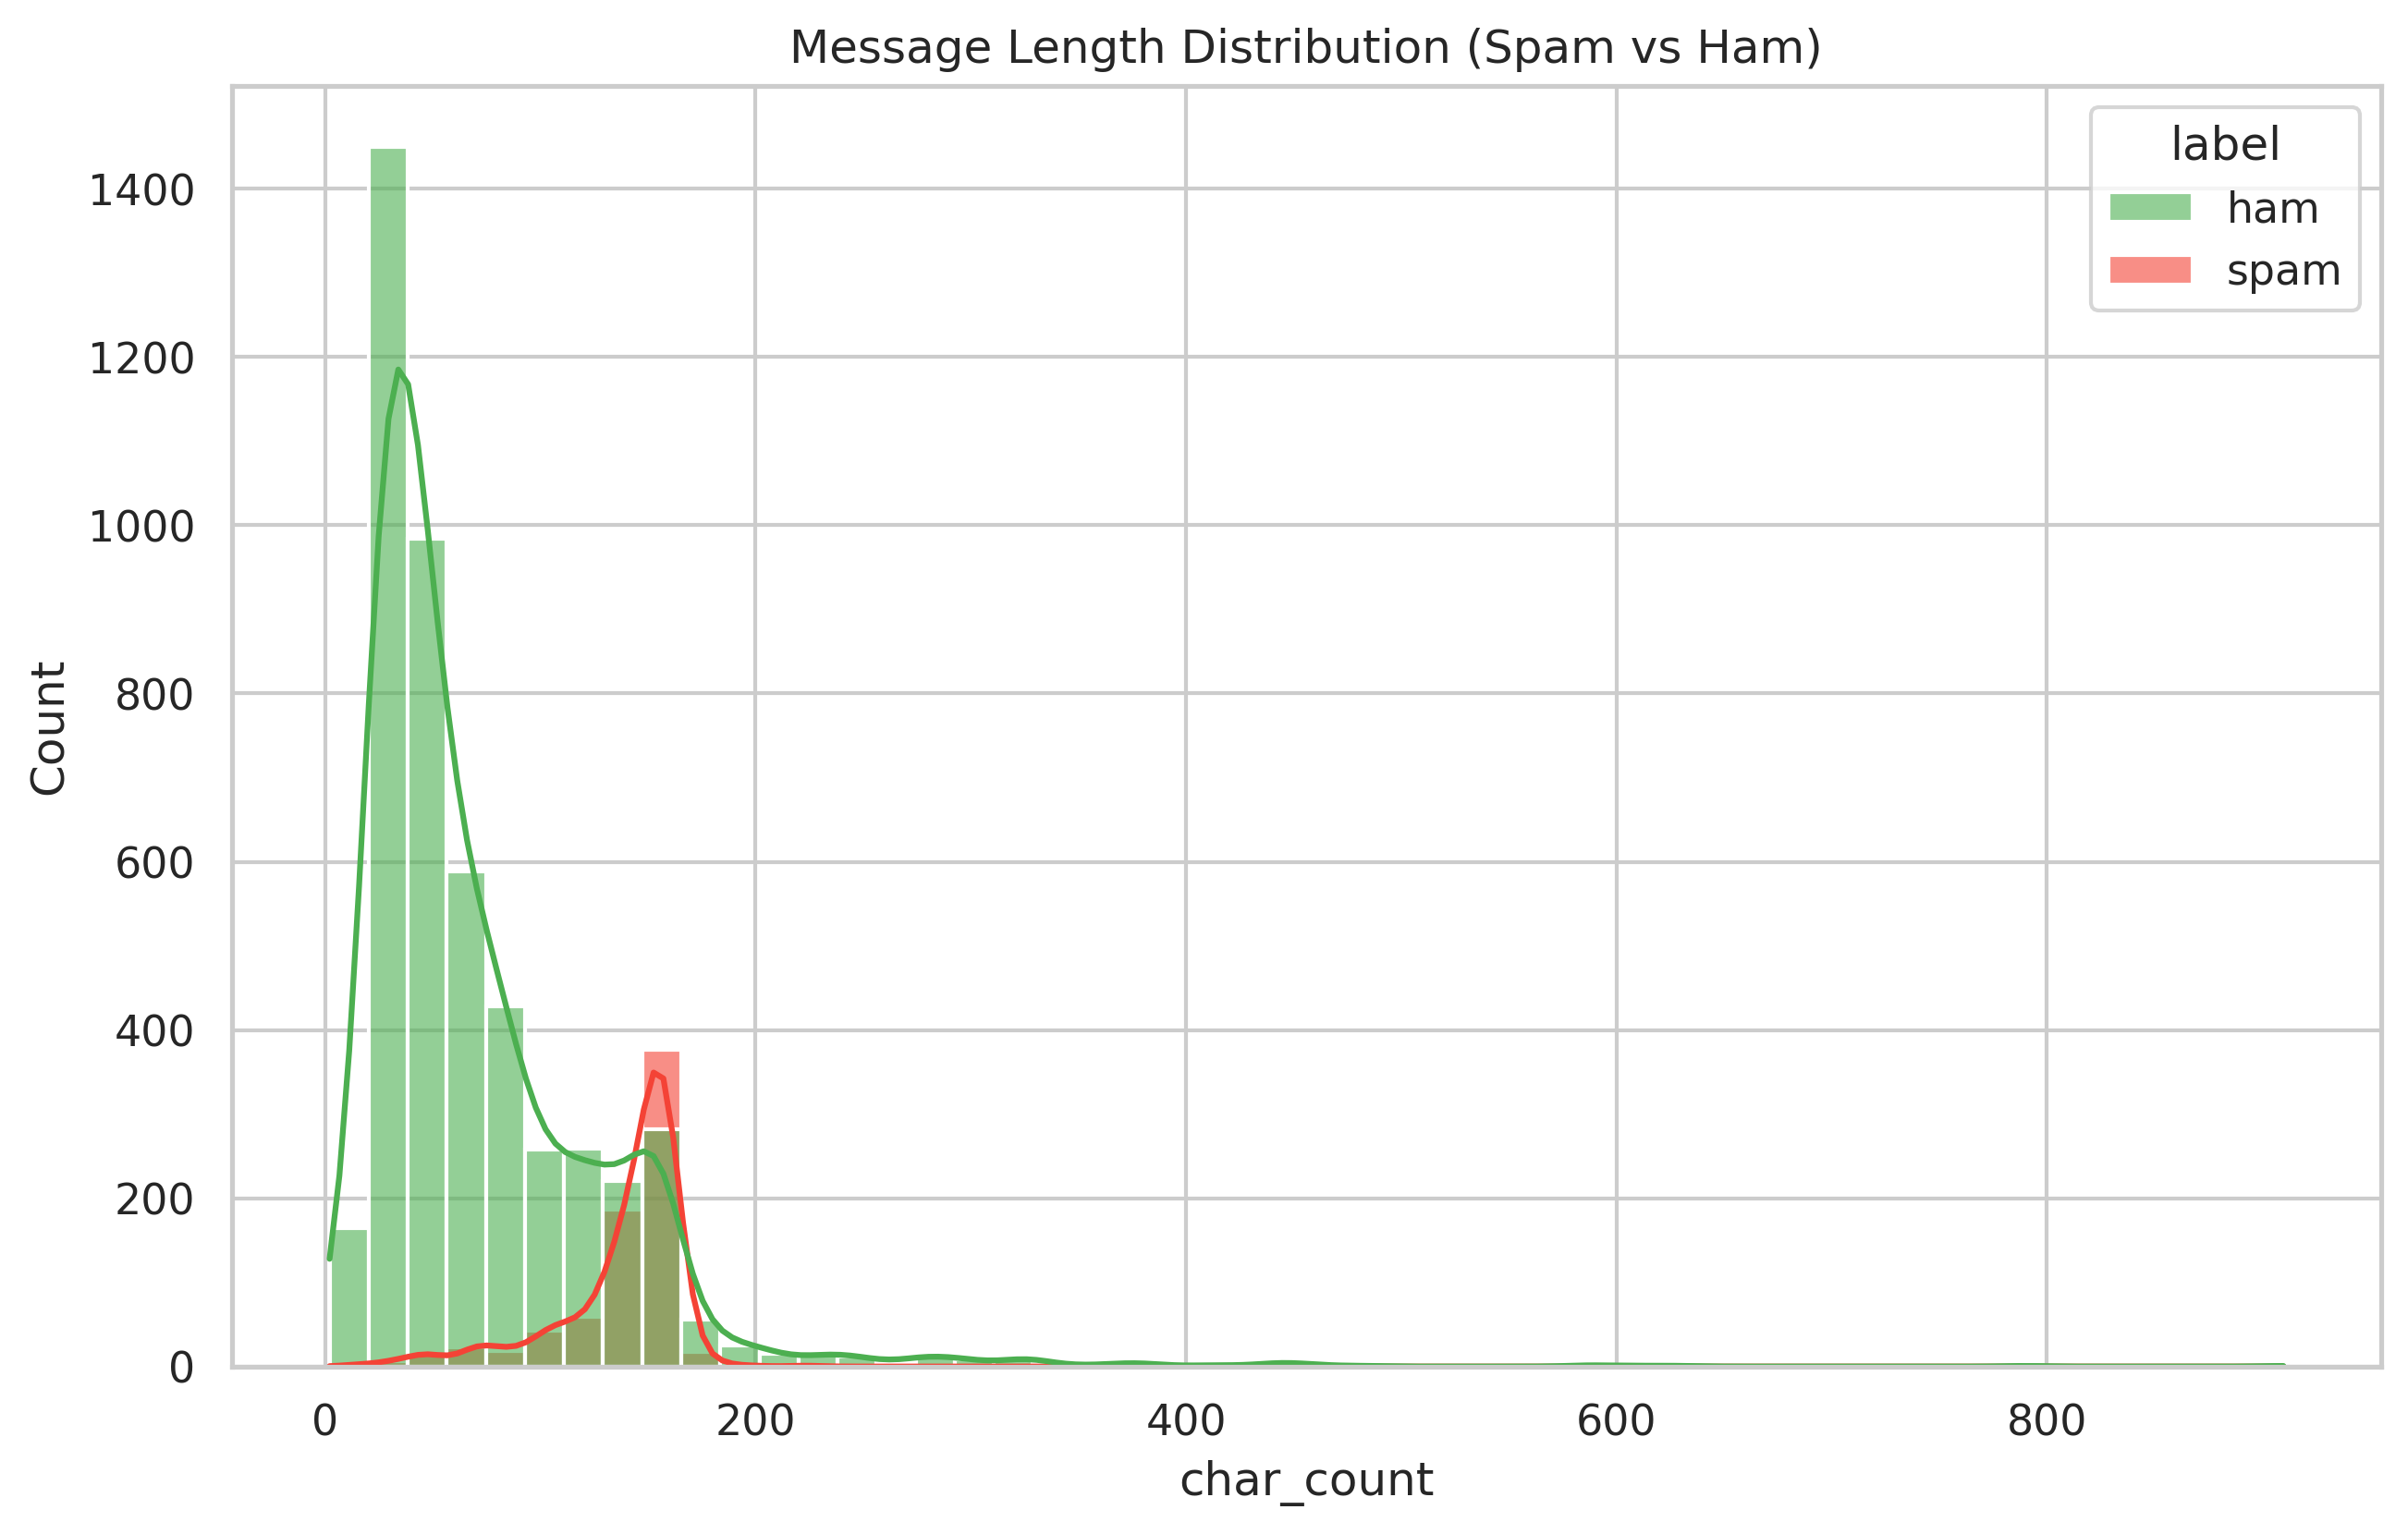
\includegraphics[width=0.92\textwidth]{images/msg_length_dist.png}
    \caption{\textbf{Figure T2} --- Message Length Distribution: Histogram (left) and Boxplot (right) comparing Ham vs.\ Spam.
    \textit{Code:} \texttt{df['length'] = df['text'].apply(len)}, then \texttt{plt.hist()} and \texttt{df.boxplot(column='length', by='label')}.}
    \label{fig:text_length}
\end{figure}

\subsection{Vocabulary and Word Cloud Analysis}

Word clouds (Figure T3 below) were generated using the \texttt{WordCloud} library on each label's concatenated text. The visual contrast is immediately striking:

\begin{itemize}
    \item \textbf{Ham (green):} Dominated by everyday conversational words --- \textit{call}, \textit{come}, \textit{going}, \textit{time}, \textit{day}, \textit{know}, \textit{will}. These reflect the informal, relational nature of legitimate SMS exchanges.
    \item \textbf{Spam (red):} Dominated by promotional language --- \textit{free}, \textit{win}, \textit{prize}, \textit{claim}, \textit{txt}, \textit{urgent}, \textit{call}. Notably, ``call'' appears in both corpora but in fundamentally different contexts: personal calls in ham vs.\ calls to premium-rate numbers in spam.
\end{itemize}

\begin{figure}[H]
    \centering
    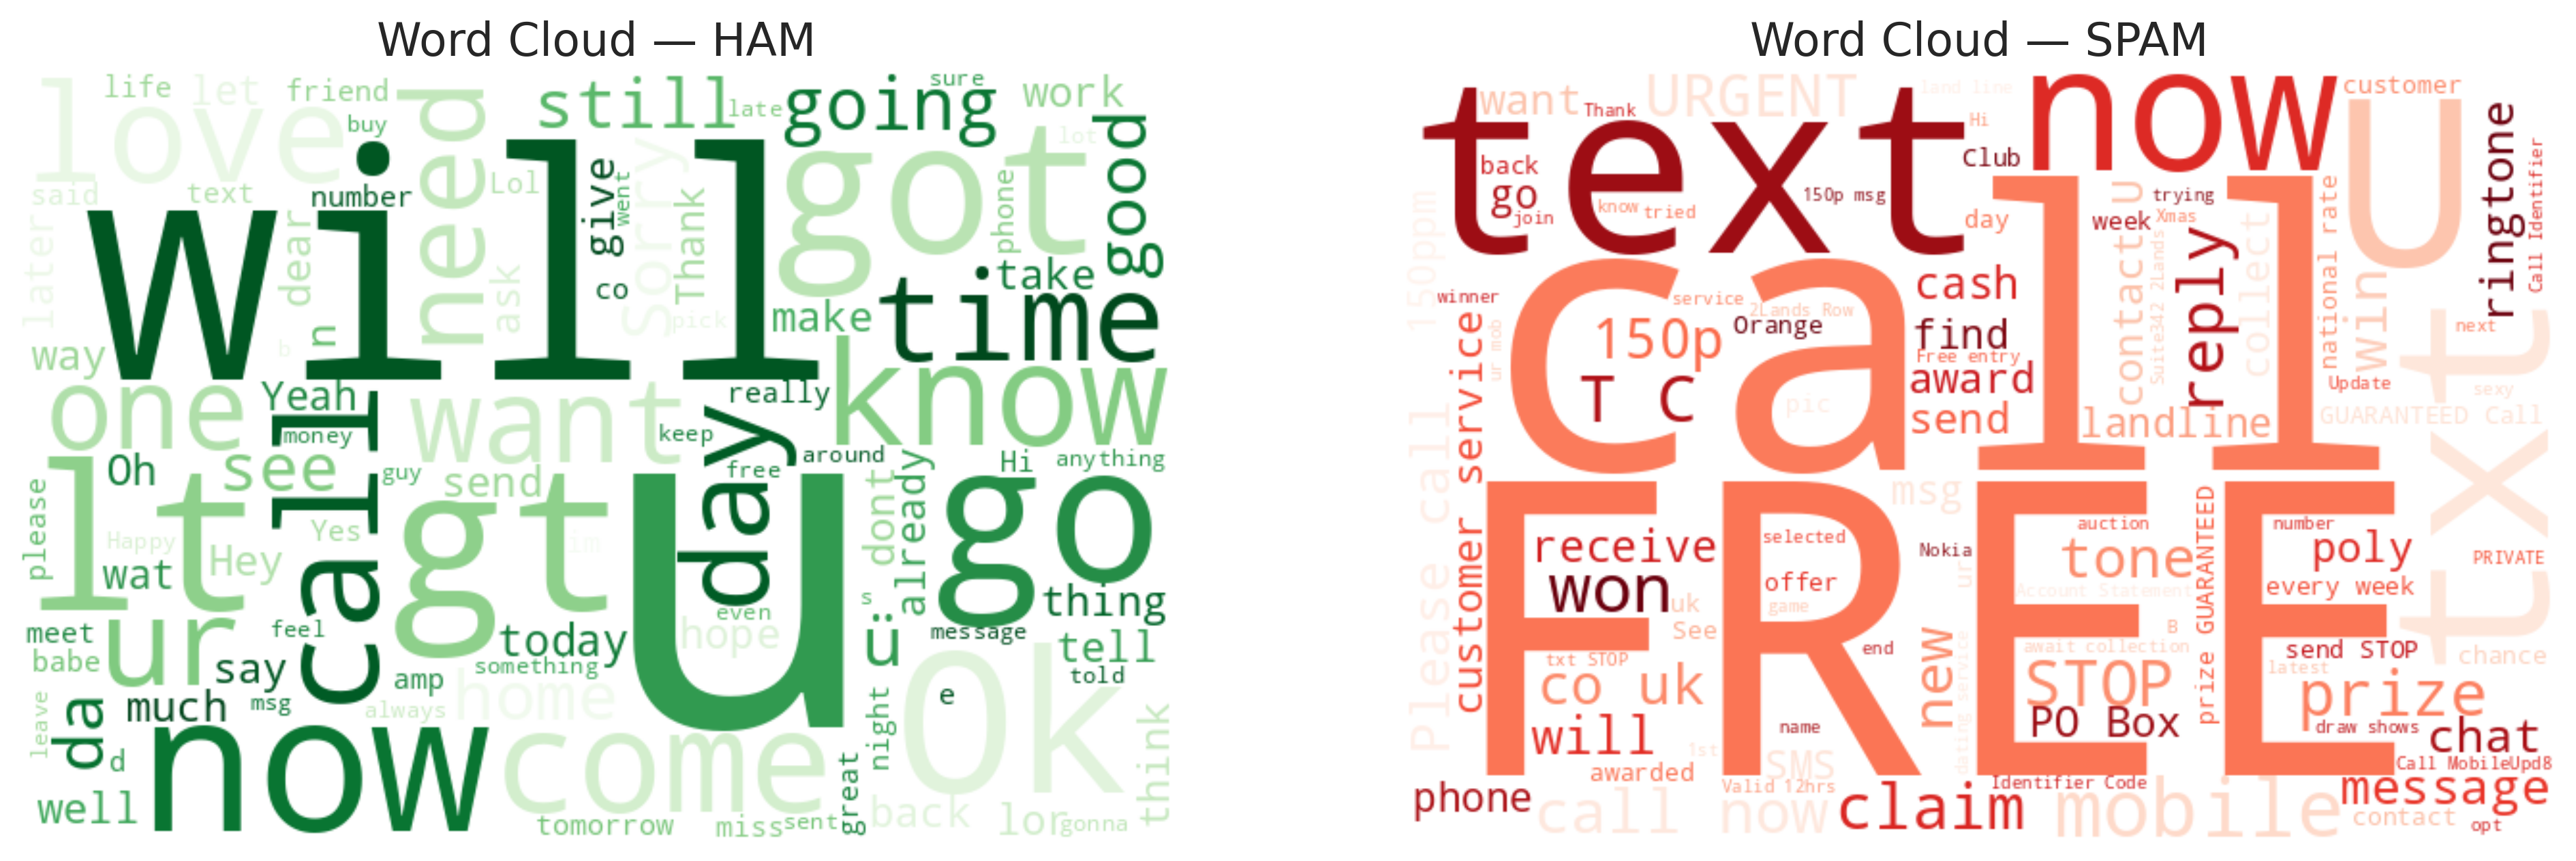
\includegraphics[width=0.90\textwidth]{images/wordclouds.png}
    \caption{\textbf{Figure T3} --- Word Clouds for Ham (left, green) and Spam (right, red).
    \textit{Code:} \texttt{WordCloud(max\_words=200, background\_color='white').generate(text)} per label.}
    \label{fig:wordclouds}
\end{figure}

\subsection{Token Frequency Analysis}

\subsubsection*{Step 1 --- Top Overall Tokens (Before Preprocessing)}

Figure T4 below shows the 20 most frequent tokens across the full corpus before any preprocessing. The list is dominated by high-frequency function words (``I'', ``to'', ``a'', ``u'', ``you'') that carry no discriminative power between classes. This motivates the stopword removal step.

\begin{figure}[H]
    \centering
    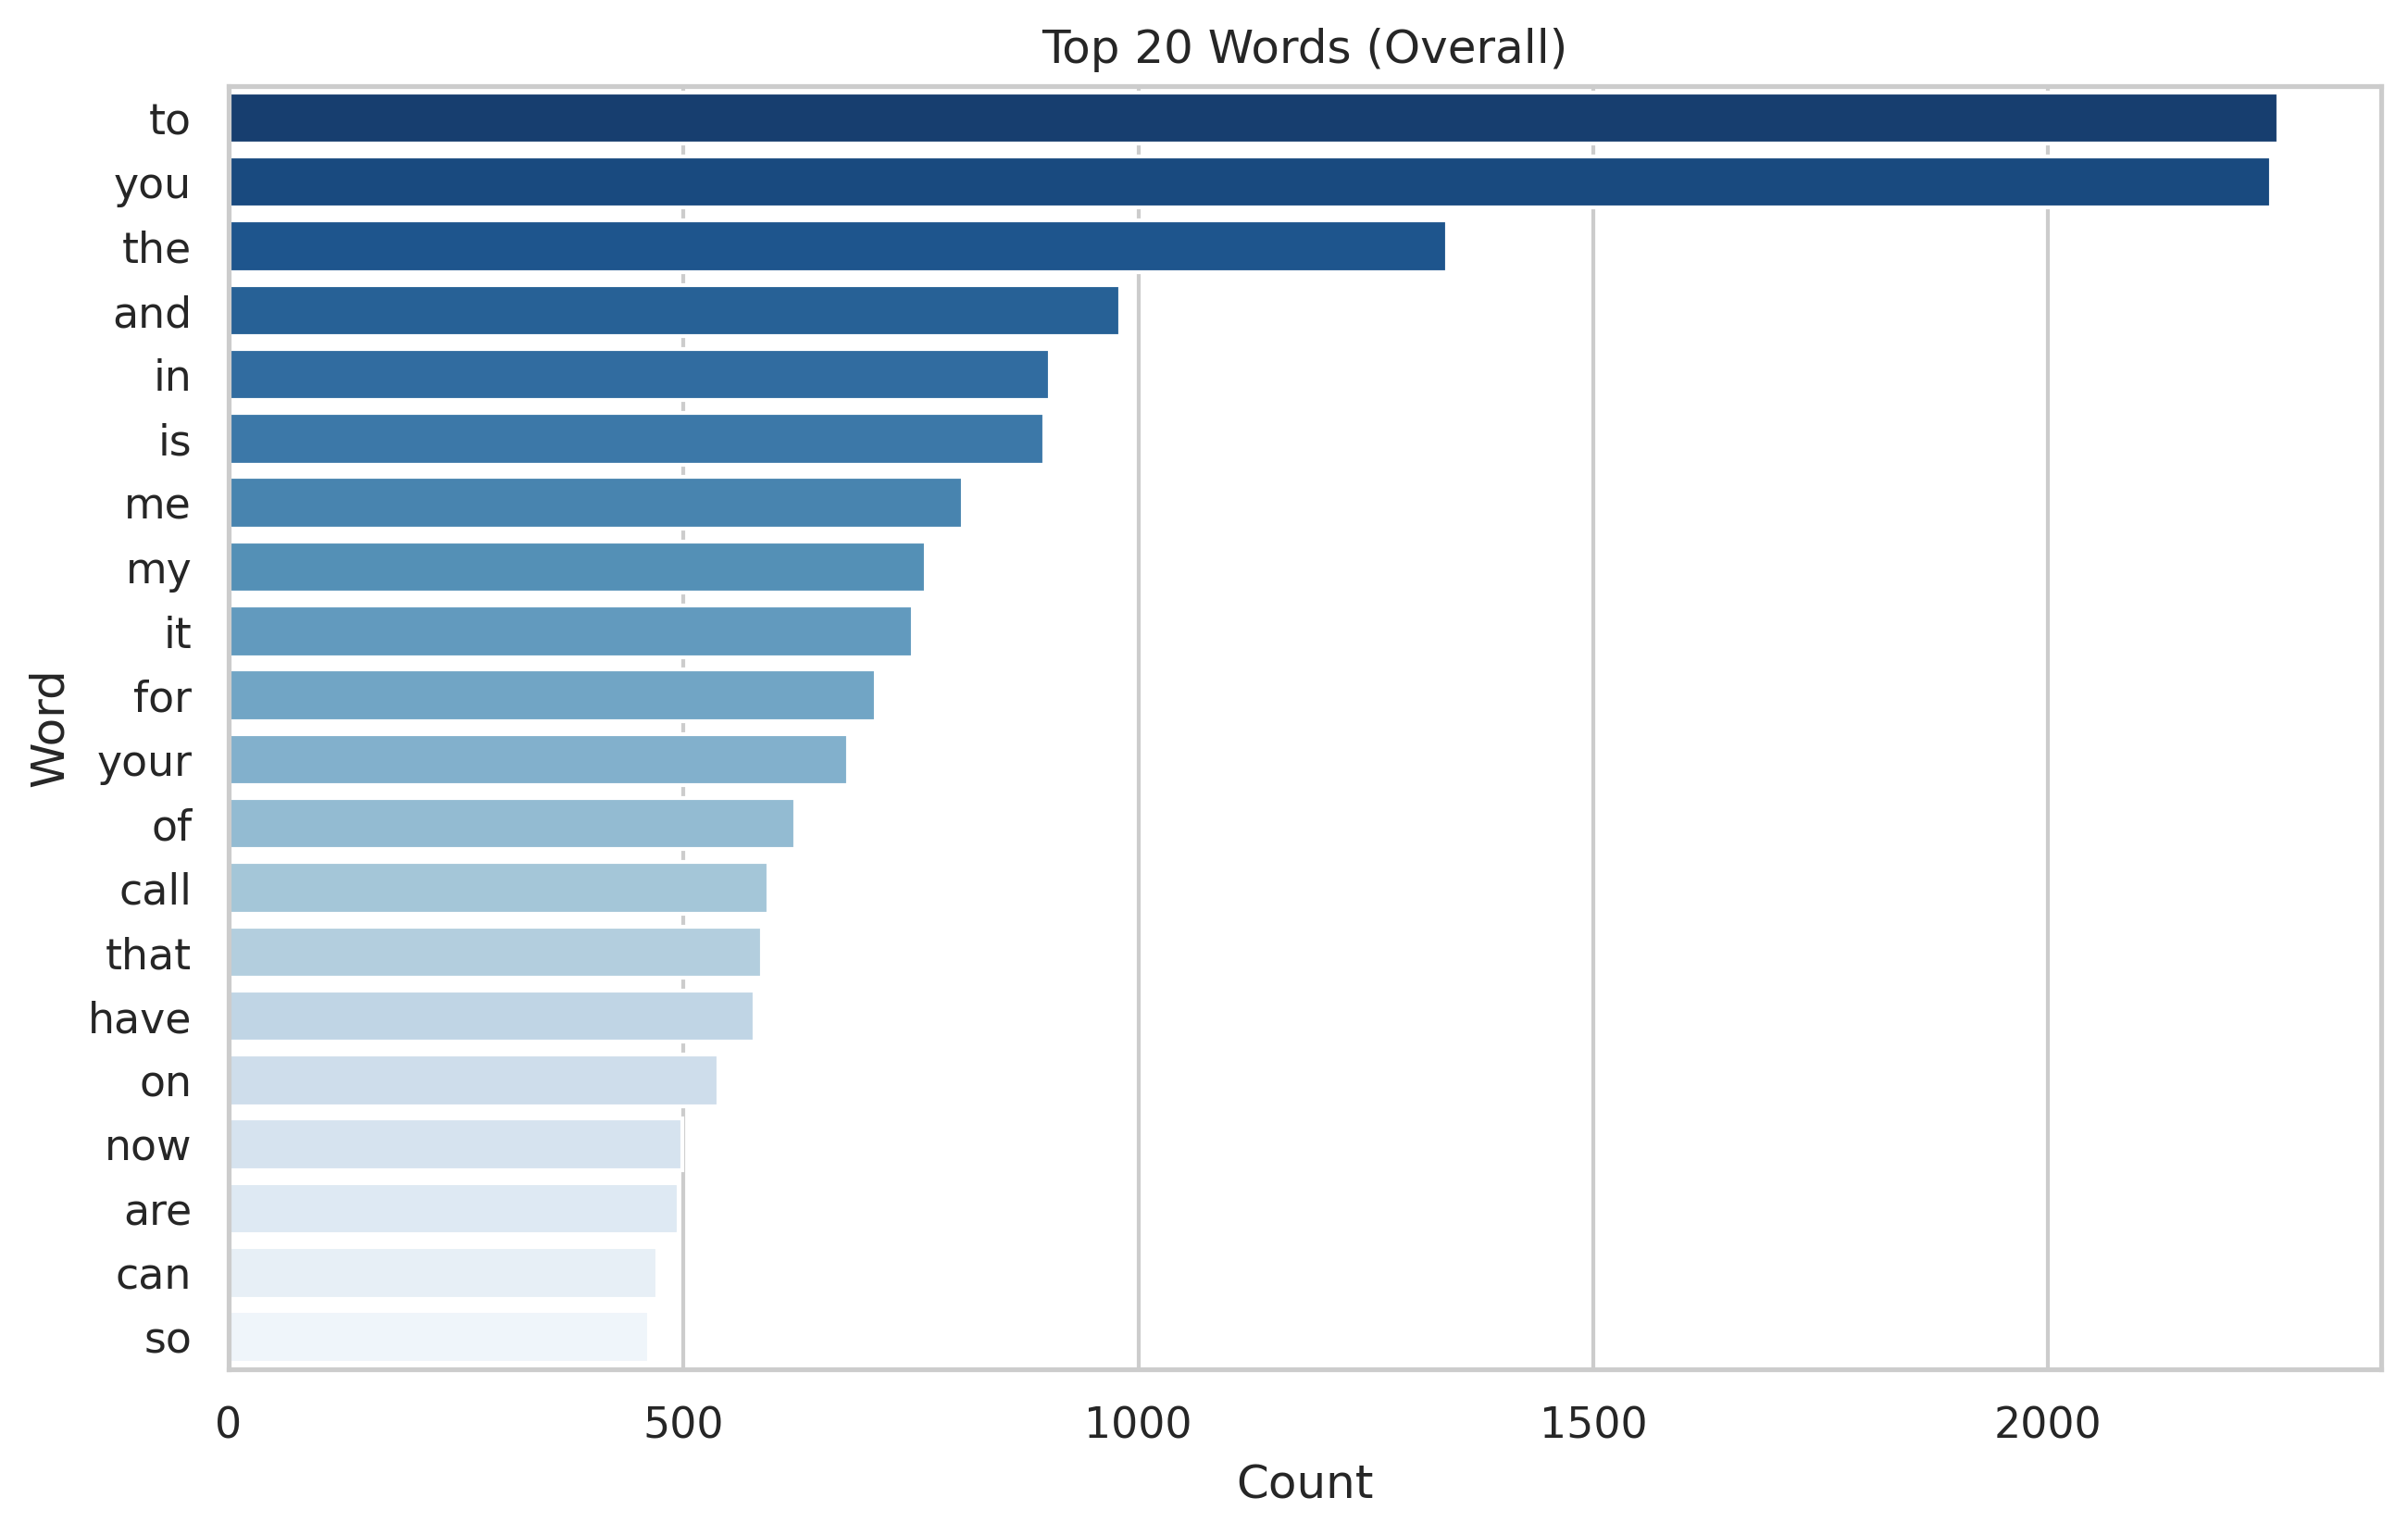
\includegraphics[width=0.85\textwidth]{images/top_overall.png}
    \caption{\textbf{Figure T4} --- Top 20 Most Frequent Tokens across the Full Corpus (stopwords included).
    \textit{Code:} \texttt{Counter(all\_tokens).most\_common(20)}.}
    \label{fig:text_top_overall}
\end{figure}

\subsubsection*{Step 2 --- Identifying Stopwords}

Figure T5 below isolates the top stopwords found in the corpus. Their dominance in the raw frequency list confirms that stopword removal is a necessary preprocessing step.

\begin{figure}[H]
    \centering
    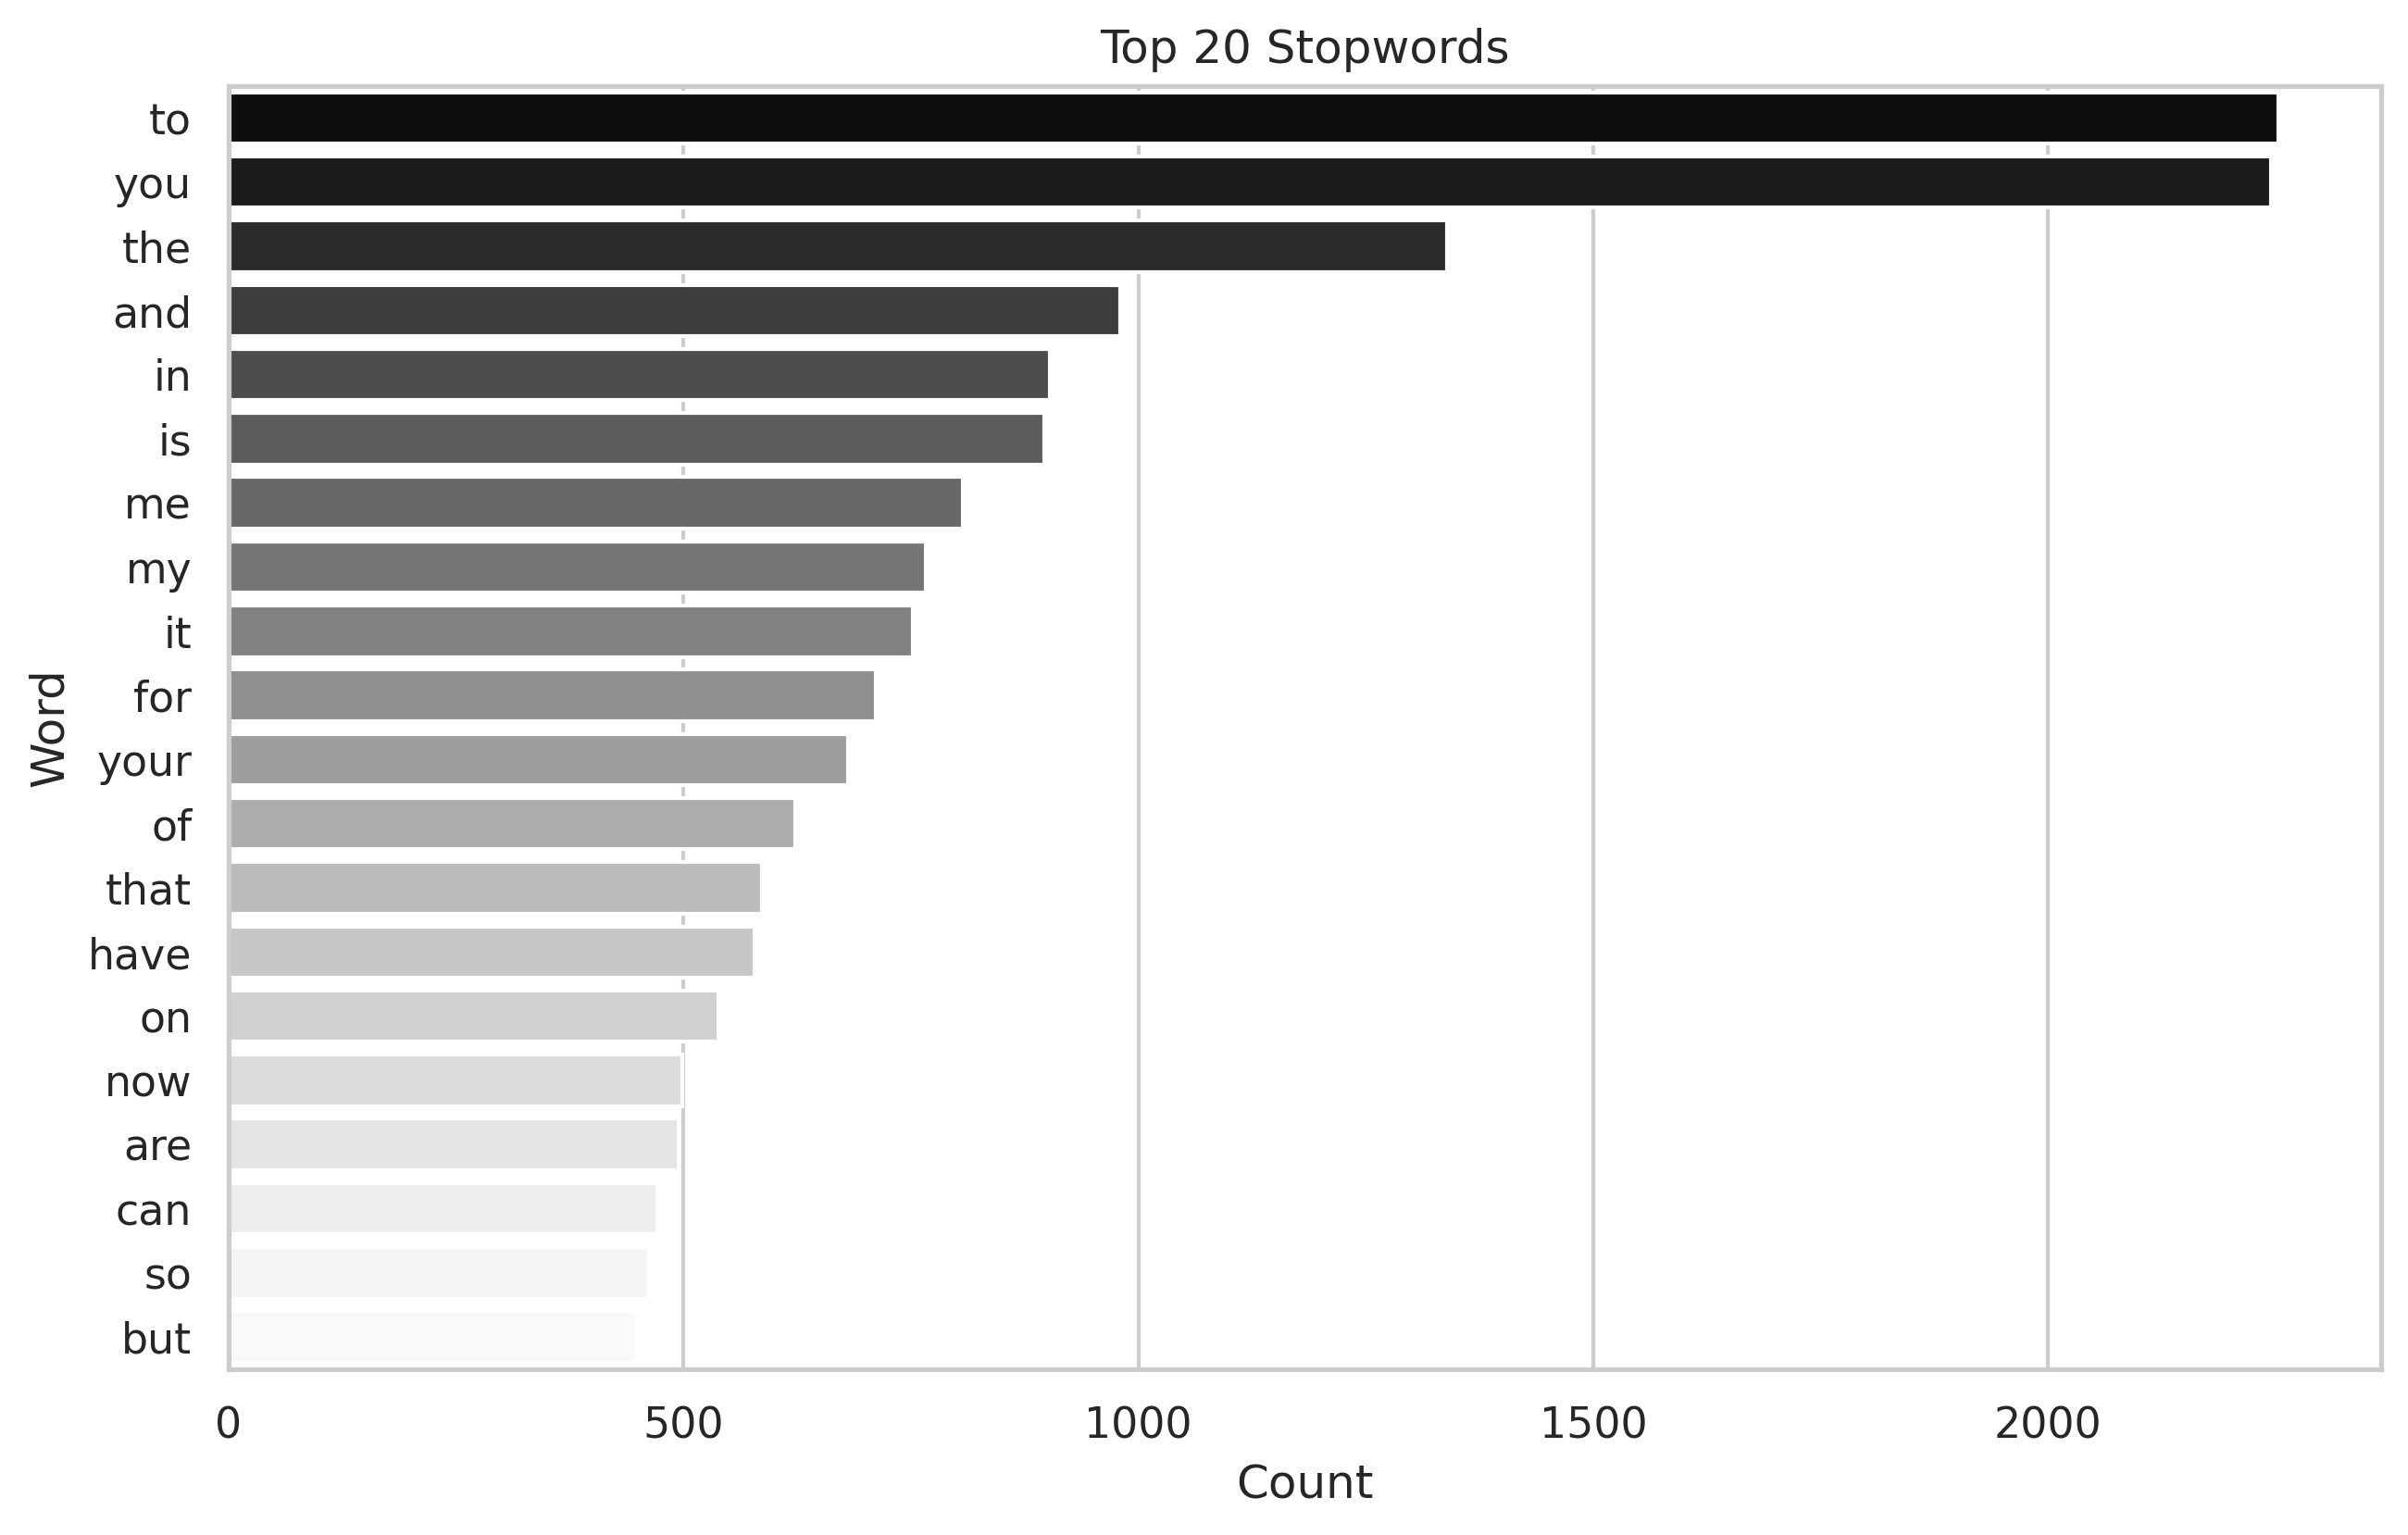
\includegraphics[width=0.85\textwidth]{images/top_stopwords.png}
    \caption{\textbf{Figure T5} --- Top Stopwords in the Corpus. Removing these exposes the discriminative vocabulary.
    \textit{Code:} Frequency count on a curated stopword set intersected with all tokens.}
    \label{fig:text_top_stopwords}
\end{figure}

\subsubsection*{Step 3 --- Top Discriminative Tokens (After Stopword Removal)}

Figure T6 below shows the class-specific top tokens after removing standard English stopwords. The class separation is clear:

\begin{itemize}
    \item \textbf{Spam-associated:} \textit{free}, \textit{win}, \textit{prize}, \textit{claim}, \textit{txt}, \textit{mobile} --- promotional, action-driving vocabulary.
    \item \textbf{Ham-associated:} \textit{call}, \textit{come}, \textit{good}, \textit{time}, \textit{day}, \textit{know} --- natural everyday conversational terms.
\end{itemize}

\begin{figure}[H]
    \centering
    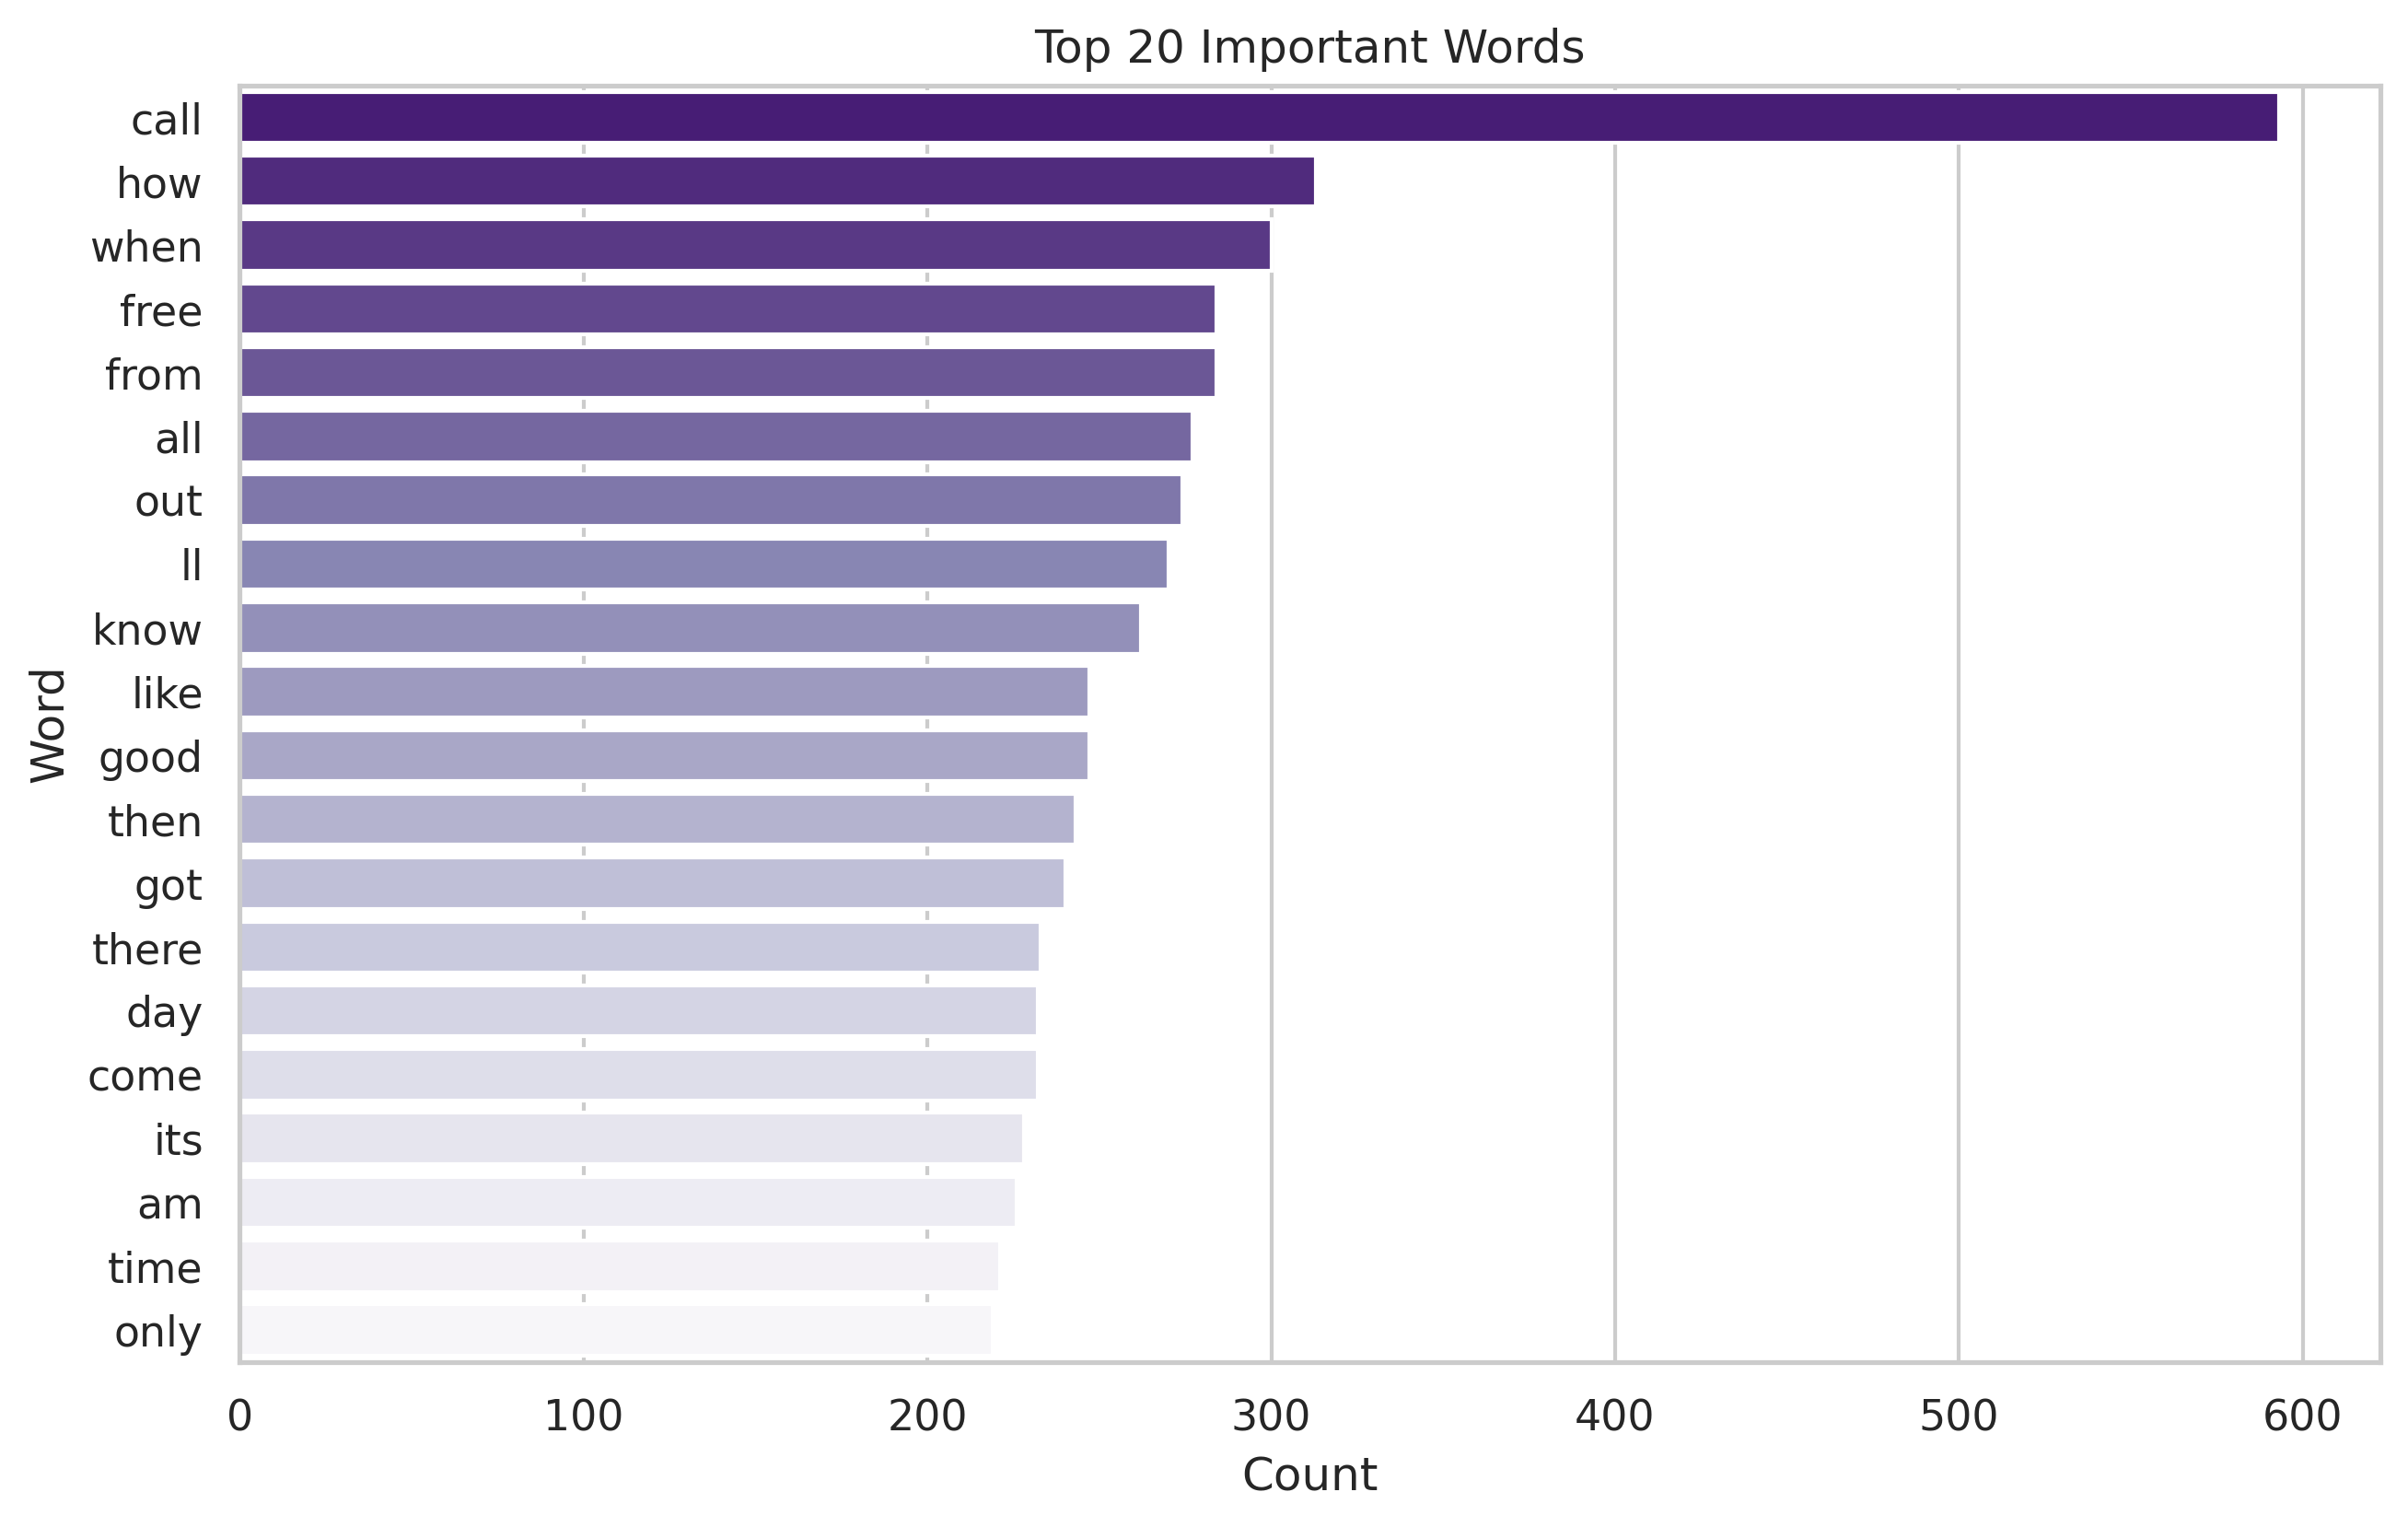
\includegraphics[width=0.85\textwidth]{images/top_important.png}
    \caption{\textbf{Figure T6} --- Top Discriminative Tokens After Stopword Removal, split by class (ham vs.\ spam).
    \textit{Code:} \texttt{Counter(filtered\_tokens).most\_common(15)} per label subset.}
    \label{fig:text_top_important}
\end{figure}

\subsection{N-gram Analysis}

Single-token frequencies miss multi-word patterns. Figure T7 below extends the analysis to bigrams and trigrams, revealing formulaic phrase patterns unique to each class:

\begin{itemize}
    \item \textbf{Spam bigrams / trigrams:} ``free entry'', ``text to win'', ``win a prize'', ``call now'', ``cash prize'' --- short promotional formulas that function as near-perfect spam signatures.
    \item \textbf{Ham bigrams / trigrams:} ``going to'', ``can I'', ``let me know'', ``talk to you'' --- natural conversational connectors typical of personal SMS dialogue.
\end{itemize}

N-gram features (e.g., a TF-IDF vectoriser with \texttt{ngram\_range=(1,2)}) are expected to be highly informative for this classification task, outperforming unigram-only approaches.

\begin{figure}[H]
    \centering
    
\includegraphics[width=0.95\textwidth]{images/top_bigrams.png}
    \caption{\textbf{Figure T7} --- Bigram and Trigram Frequency Analysis by Label (Ham vs.\ Spam).
    \textit{Code:} \texttt{Counter(ngrams(tokens, n)).most\_common(12)} per label, displayed with \texttt{ax.barh()}.}
    \label{fig:text_bigrams}
\end{figure}

\subsection{Word Count vs.\ Character Count}

Figure T8 below scatterplots the word count (number of whitespace-delimited tokens) against character count for each message, coloured by label. The two classes form visually separable clusters:

\begin{itemize}
    \item \textbf{Ham cluster:} Dispersed cloud at low-to-moderate word and character counts, with a long tail of very long messages (the multi-segment personal messages reaching 910 chars).
    \item \textbf{Spam cluster:} Compact, dense region at moderate-to-high word counts and moderate character counts (roughly 100--224 chars), consistent with templated messages optimised for the 160-char SMS limit.
\end{itemize}

The visual separation confirms that \textbf{both word count and character count are strong discriminating features} even without any NLP preprocessing.

\begin{figure}[H]
    \centering
    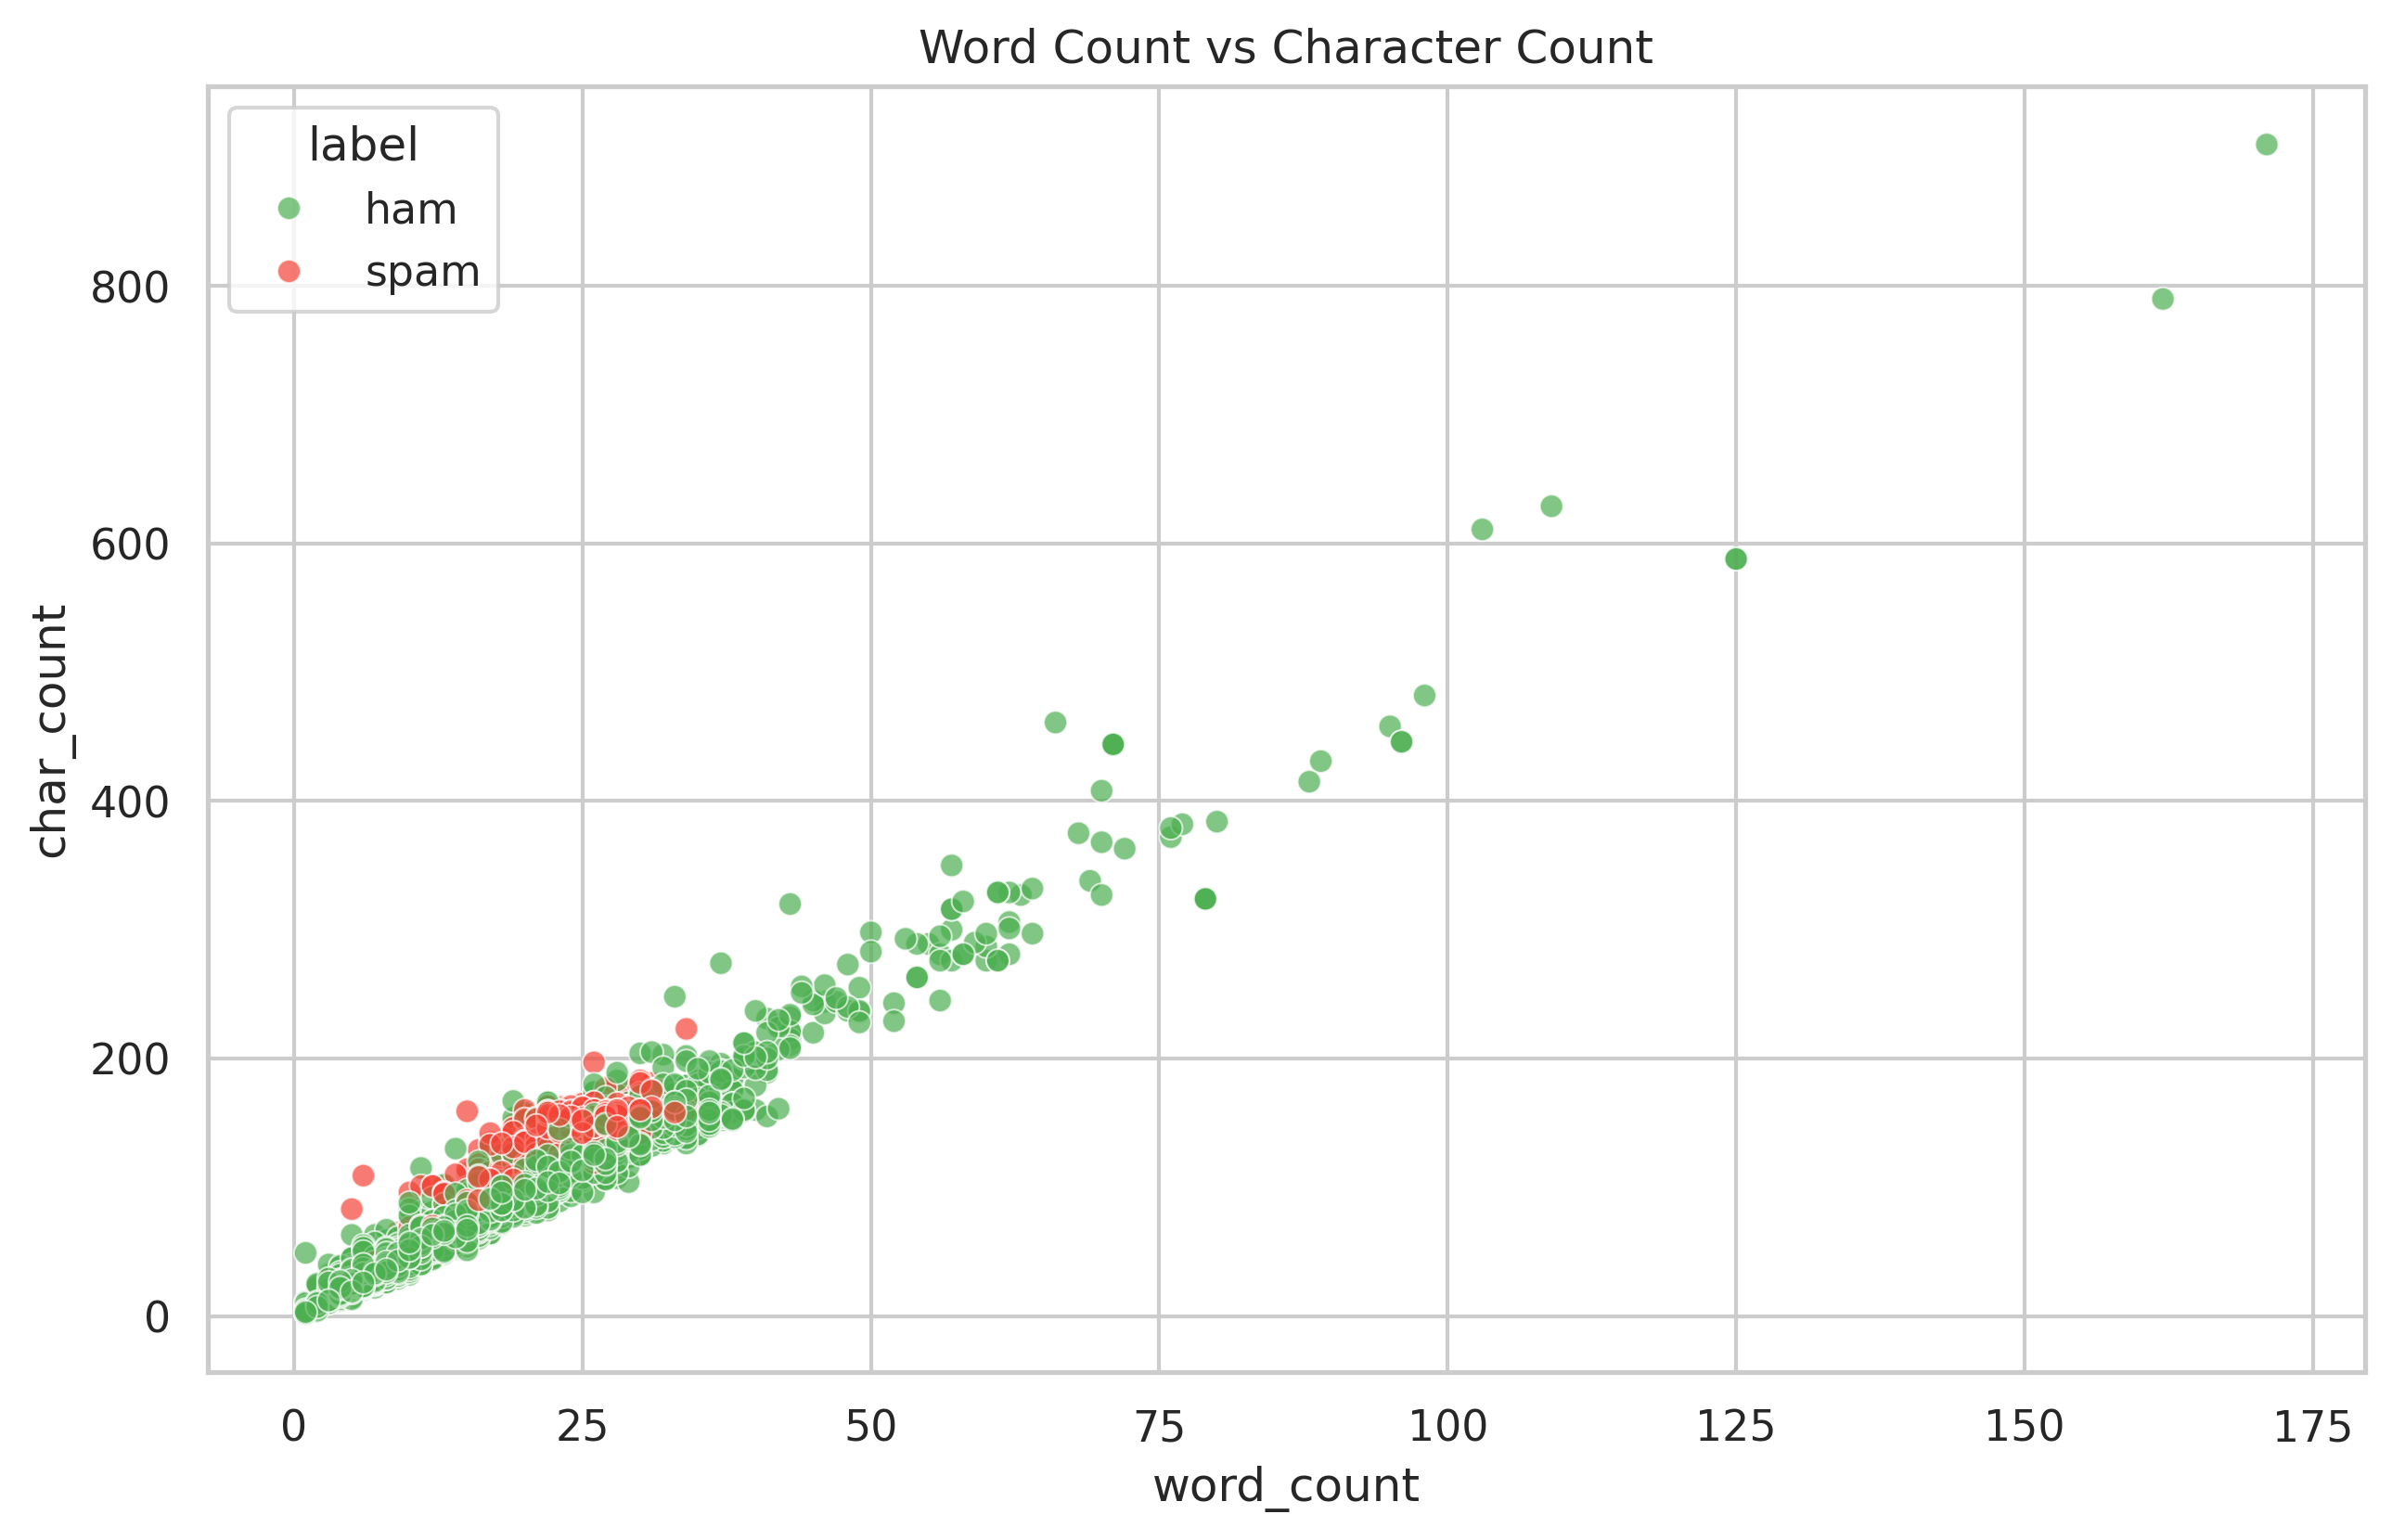
\includegraphics[width=0.75\textwidth]{images/word_vs_char.png}
    \caption{\textbf{Figure T8} --- Word Count vs.\ Character Count per message, coloured by label.
    \textit{Code:} \texttt{df['n\_words'] = df['text'].str.split().str.len()}, then \texttt{plt.scatter()}.}
    \label{fig:text_word_vs_char}
\end{figure}

% ---------------------------------------------------------
\subsection{Special Character and URL Feature Analysis}

Beyond raw length and vocabulary, \textbf{structural features} of the message text reveal strong spam signals. The following six binary or ratio features were engineered and compared between classes:

\begin{itemize}
    \item \textbf{Upper Ratio:} Fraction of characters that are uppercase.
    \item \textbf{Exclamation:} Number of \texttt{!} characters per message.
    \item \textbf{Dollar:} Number of \texttt{\$} characters per message.
    \item \textbf{Has URL:} 1 if the message contains \texttt{http}, \texttt{www}, or \texttt{.com}; else 0.
    \item \textbf{Has Phone:} 1 if the message contains a sequence of $\geq 5$ digits (phone number); else 0.
    \item \textbf{Has Number:} 1 if any digit appears in the message; else 0.
\end{itemize}

Table T2 below summarises the mean values per class, and Figure T9 visualises each feature side-by-side:

\begin{table}[H]
\centering
\caption{\textbf{Table T2} --- Mean Special Feature Values by Label}
\label{tab:text_features}
\begin{tabular}{lrr}
\hline
\textbf{Feature} & \textbf{Ham} & \textbf{Spam} \\
\hline
Upper Ratio  & 0.059 & 0.111 \\
Exclamation  & 0.177 & 0.730 \\
Dollar (\$)  & 0.000 & 0.000 \\
Has URL      & 0.004 & 0.162 \\
Has Phone    & 0.001 & 0.756 \\
Has Number   & 0.157 & 0.948 \\
\hline
\end{tabular}
\end{table}

\begin{figure}[H]
    \centering
    
\includegraphics[width=0.95\textwidth]{images/text_features.png}
    \caption{\textbf{Figure T9} --- Special Feature Comparison: Ham (green) vs.\ Spam (red) for 6 engineered features. Bar height = mean value across all messages in that class.
    \textit{Code:} Feature engineering via regex and \texttt{str.count()}, then \texttt{groupby('label').mean()} and \texttt{plt.bar()}.}
    \label{fig:text_features}
\end{figure}

Key observations from Figure T9:
\begin{itemize}
    \item \textbf{Has Phone is the strongest discriminator:} 75.6\% of spam contains a phone number vs.\ only 0.06\% of ham. A phone number in a message is an almost certain spam indicator.
    \item \textbf{Has Number is nearly universal in spam:} 94.8\% of spam messages contain at least one digit (prize amounts, phone numbers, competition codes) vs.\ only 15.7\% of ham.
    \item \textbf{URL presence signals spam:} 16.2\% of spam contains a URL or web address vs.\ only 0.35\% of ham. Spam links typically drive recipients to phishing or premium-rate sites.
    \item \textbf{Exclamation marks signal urgency:} Spam uses exclamation marks $4\times$ more than ham (mean 0.73 vs.\ 0.18), consistent with urgency-driven promotional language.
    \item \textbf{Uppercase emphasis:} Spam has nearly $2\times$ the uppercase ratio (0.111 vs.\ 0.059), reflecting the ``SHOUTING'' style of spam (e.g., ``WIN NOW'', ``FREE PRIZE'').
    \item \textbf{Dollar sign inconclusive:} Both classes show near-zero dollar sign usage in this dataset --- it is not a useful feature here.
\end{itemize}

% ---------------------------------------------------------
\subsection{Vocabulary Richness Analysis (Type-Token Ratio)}

The \textbf{Type-Token Ratio (TTR)} measures vocabulary richness: it is the ratio of unique words (types) to total words (tokens). A higher TTR indicates more diverse, less repetitive language.

\begin{table}[H]
\centering
\caption{\textbf{Table T3} --- Vocabulary Richness Comparison: Ham vs.\ Spam}
\label{tab:text_ttr}
\begin{tabular}{lrrr}
\hline
\textbf{Label} & \textbf{Total Words} & \textbf{Unique Words} & \textbf{TTR} \\
\hline
Ham  & 69{,}905 & 6{,}709 & 0.0960 \\
Spam & 15{,}819 & 1{,}940 & 0.1226 \\
\hline
\end{tabular}
\end{table}

Figure T10 below visualises three vocabulary richness metrics side-by-side:

\begin{figure}[H]
    \centering
    
\includegraphics[width=0.95\textwidth]{images/text_vocab_richness.png}
    \caption{\textbf{Figure T10} --- Vocabulary Richness Analysis: Unique Word Count (left), Type-Token Ratio / TTR (centre), and Average Word Length (right) for Ham vs.\ Spam.
    \textit{Code:} \texttt{len(set(tokens)) / len(tokens)} for TTR; \texttt{np.mean([len(w) for w in tokens])} for avg word length.}
    \label{fig:text_vocab_richness}
\end{figure}

Key observations from Figure T10 and Table T3 above:
\begin{itemize}
    \item \textbf{Ham has a larger raw vocabulary} (6{,}709 unique words vs.\ 1{,}940 for spam), reflecting the more open-ended, natural language of legitimate messages.
    \item \textbf{Spam has a higher TTR} (0.1226 vs.\ 0.0960) despite a smaller absolute vocabulary. This is because ham's corpus is much larger (69{,}905 tokens vs.\ 15{,}819) --- the TTR naturally decreases with corpus size as common words repeat more. The higher spam TTR reflects its \emph{smaller corpus size}, not greater vocabulary diversity.
    \item \textbf{Spam uses longer words on average} (4.97 chars/word vs.\ 4.17 for ham), likely due to promotional terms like ``congratulations'', ``guaranteed'', ``unsubscribe''.
    \item \textbf{Implication:} TTR is corpus-size dependent and should be used cautiously as a standalone feature; it is more reliable when computed on messages of equal length.
\end{itemize}

% ---------------------------------------------------------
\subsection{Key Findings}

\begin{importantbox}
\textbf{Summary of Text EDA Key Findings:}
\begin{itemize}
    \item \textbf{Class imbalance:} Ham (86.6\%) $\gg$ Spam (13.4\%). Naive accuracy is highly misleading; use F1 (macro), AUC-ROC, or Precision/Recall as primary metrics.
    \item \textbf{Length as a zero-cost feature:} Spam ($\sim$139 chars average) is nearly \textbf{2$\times$ longer} than ham ($\sim$72 chars). Message length provides strong discriminating power with zero preprocessing cost.
    \item \textbf{Structural spam signals (strongest first):}
    \begin{enumerate}
        \item Has Phone number: 75.6\% spam vs.\ 0.06\% ham (highest discriminative power)
        \item Has Number (any digit): 94.8\% spam vs.\ 15.7\% ham
        \item Has URL: 16.2\% spam vs.\ 0.35\% ham
        \item Exclamation marks: mean 0.73 spam vs.\ 0.18 ham
        \item Uppercase ratio: 11.1\% spam vs.\ 5.9\% ham
    \end{enumerate}
    \item \textbf{Vocabulary contrast:} Spam relies on promotional vocabulary (\textit{free, win, prize, claim, txt}); ham uses everyday conversational language. The vocabularies are largely non-overlapping for the most frequent class-specific terms.
    \item \textbf{N-gram signatures:} Spam contains formulaic phrase patterns (``free entry'', ``text to win'') absent from ham, making bigram TF-IDF features highly informative.
    \item \textbf{Vocabulary richness (TTR):} Ham has a larger absolute vocabulary (6{,}709 unique words); spam uses longer individual words (avg 4.97 chars/word vs.\ 4.17 for ham).
    \item \textbf{Recommended preprocessing pipeline:}
    \begin{enumerate}
        \item Lowercasing and whitespace-based tokenisation.
        \item Standard English stopword removal.
        \item Stemming or lemmatisation (Porter Stemmer / WordNet Lemmatiser).
        \item Removal of URLs, phone numbers, currency symbols, and special characters.
        \item Class balancing via SMOTE or class-weighted cross-entropy loss.
    \end{enumerate}
    \item \textbf{Recommended models:} TF-IDF + Logistic Regression or Na\"{i}ve Bayes as an interpretable baseline; fine-tuned DistilBERT for state-of-the-art performance.
\end{itemize}
\end{importantbox}

% =======================================================================


% =======================================================================
% =======================================================================
\section{Exploratory Data Analysis: Image Data}
\label{sec:image}

\subsection{Dataset Overview}
We utilized the \textbf{CIFAR-10} dataset (Python version), a widely adopted benchmark
for image classification research, originally developed by the Canadian Institute for
Advanced Research (CIFAR). It covers a broad range of real-world object categories and
is distributed freely for academic use.

\begin{itemize}
    \item \textbf{Source:} \href{https://www.cs.toronto.edu/~kriz/cifar.html}{Official CIFAR-10 Repository}
\end{itemize}

\begin{importantbox}
\textbf{Dataset Statistics:}
\begin{itemize}
    \item \textbf{Format:} 32$\times$32 pixels, RGB color images ($\texttt{uint8}$, pixel range $[0, 255]$).
    \item \textbf{Volume:} 50,000 training samples, consuming approximately 153 MB in memory.
    \item \textbf{Classes:} 10 distinct categories: airplane, automobile, bird, cat, deer,
    dog, frog, horse, ship, and truck.
\end{itemize}
\end{importantbox}

The sample grid in Figure IMG-1 below immediately reveals a key challenge of this dataset: the low spatial resolution (32$\times$32 px) makes several classes visually ambiguous to the human eye, most notably \texttt{cat} vs.\ \texttt{dog} and \texttt{bird} vs.\ \texttt{deer}. This serves as an early indicator that downstream models will need strong learned feature representations rather than relying on raw pixel patterns.

\begin{figure}[H]
    \centering
    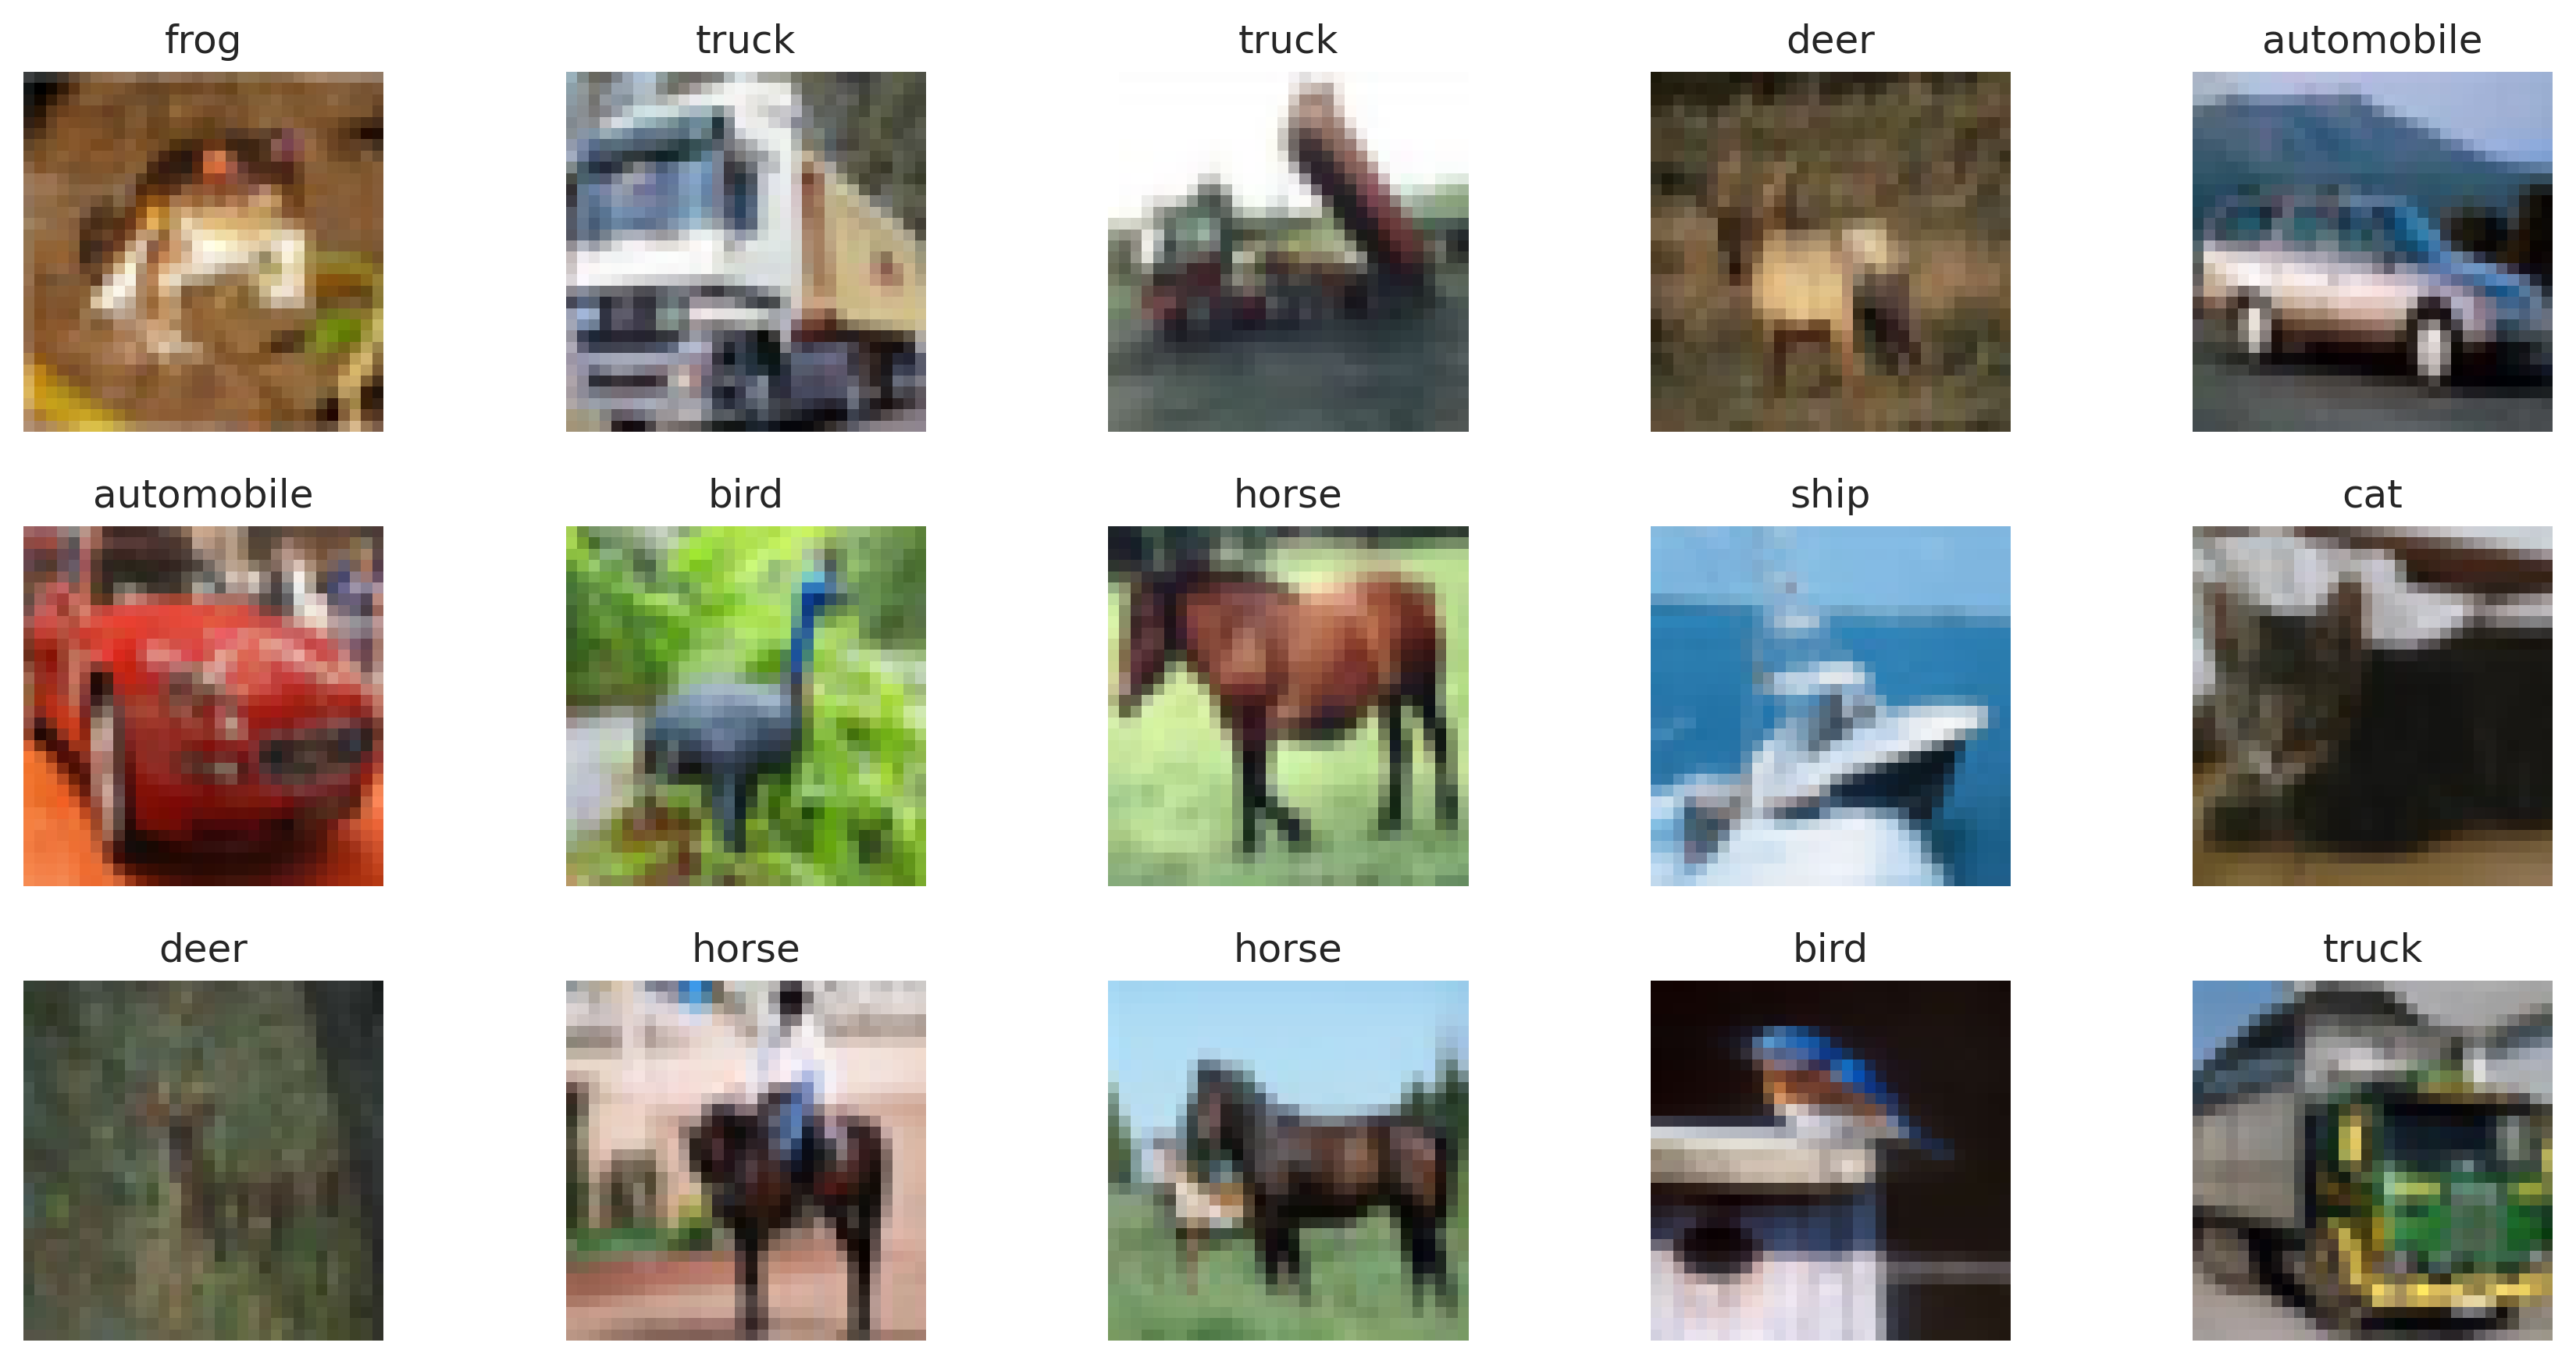
\includegraphics[width=0.85\textwidth]{images/cifar_samples.png}
    \caption{\textbf{Figure IMG-1} --- Random sample images from CIFAR-10 across all 10 classes. The small 32$\times$32 resolution makes fine-grained class boundaries (e.g.\ \texttt{cat} vs.\ \texttt{dog}) difficult to resolve even by eye.
    \textit{Code:} \texttt{plt.imshow(images[idx])} on random indices per class.}
    \label{fig:cifar_samples}
\end{figure}

\subsection{Class Distribution and Balance}

As shown in Figure IMG-2 below, CIFAR-10 contains exactly \textbf{5,000
training images per class}, yielding a perfectly uniform distribution across all 10
categories. This is a deliberate design property of the dataset, and it has two
important consequences for downstream modelling:

\begin{itemize}
    \item \textbf{No class imbalance:} Standard cross-entropy loss can be used directly
    without class weighting or oversampling strategies such as SMOTE.
    \item \textbf{Equal representation:} Every class contributes equally to any
    aggregate statistic computed over the full dataset (e.g.\ global pixel mean),
    so channel-level normalization values are not biased toward any single category.
\end{itemize}

\begin{figure}[H]
    \centering
    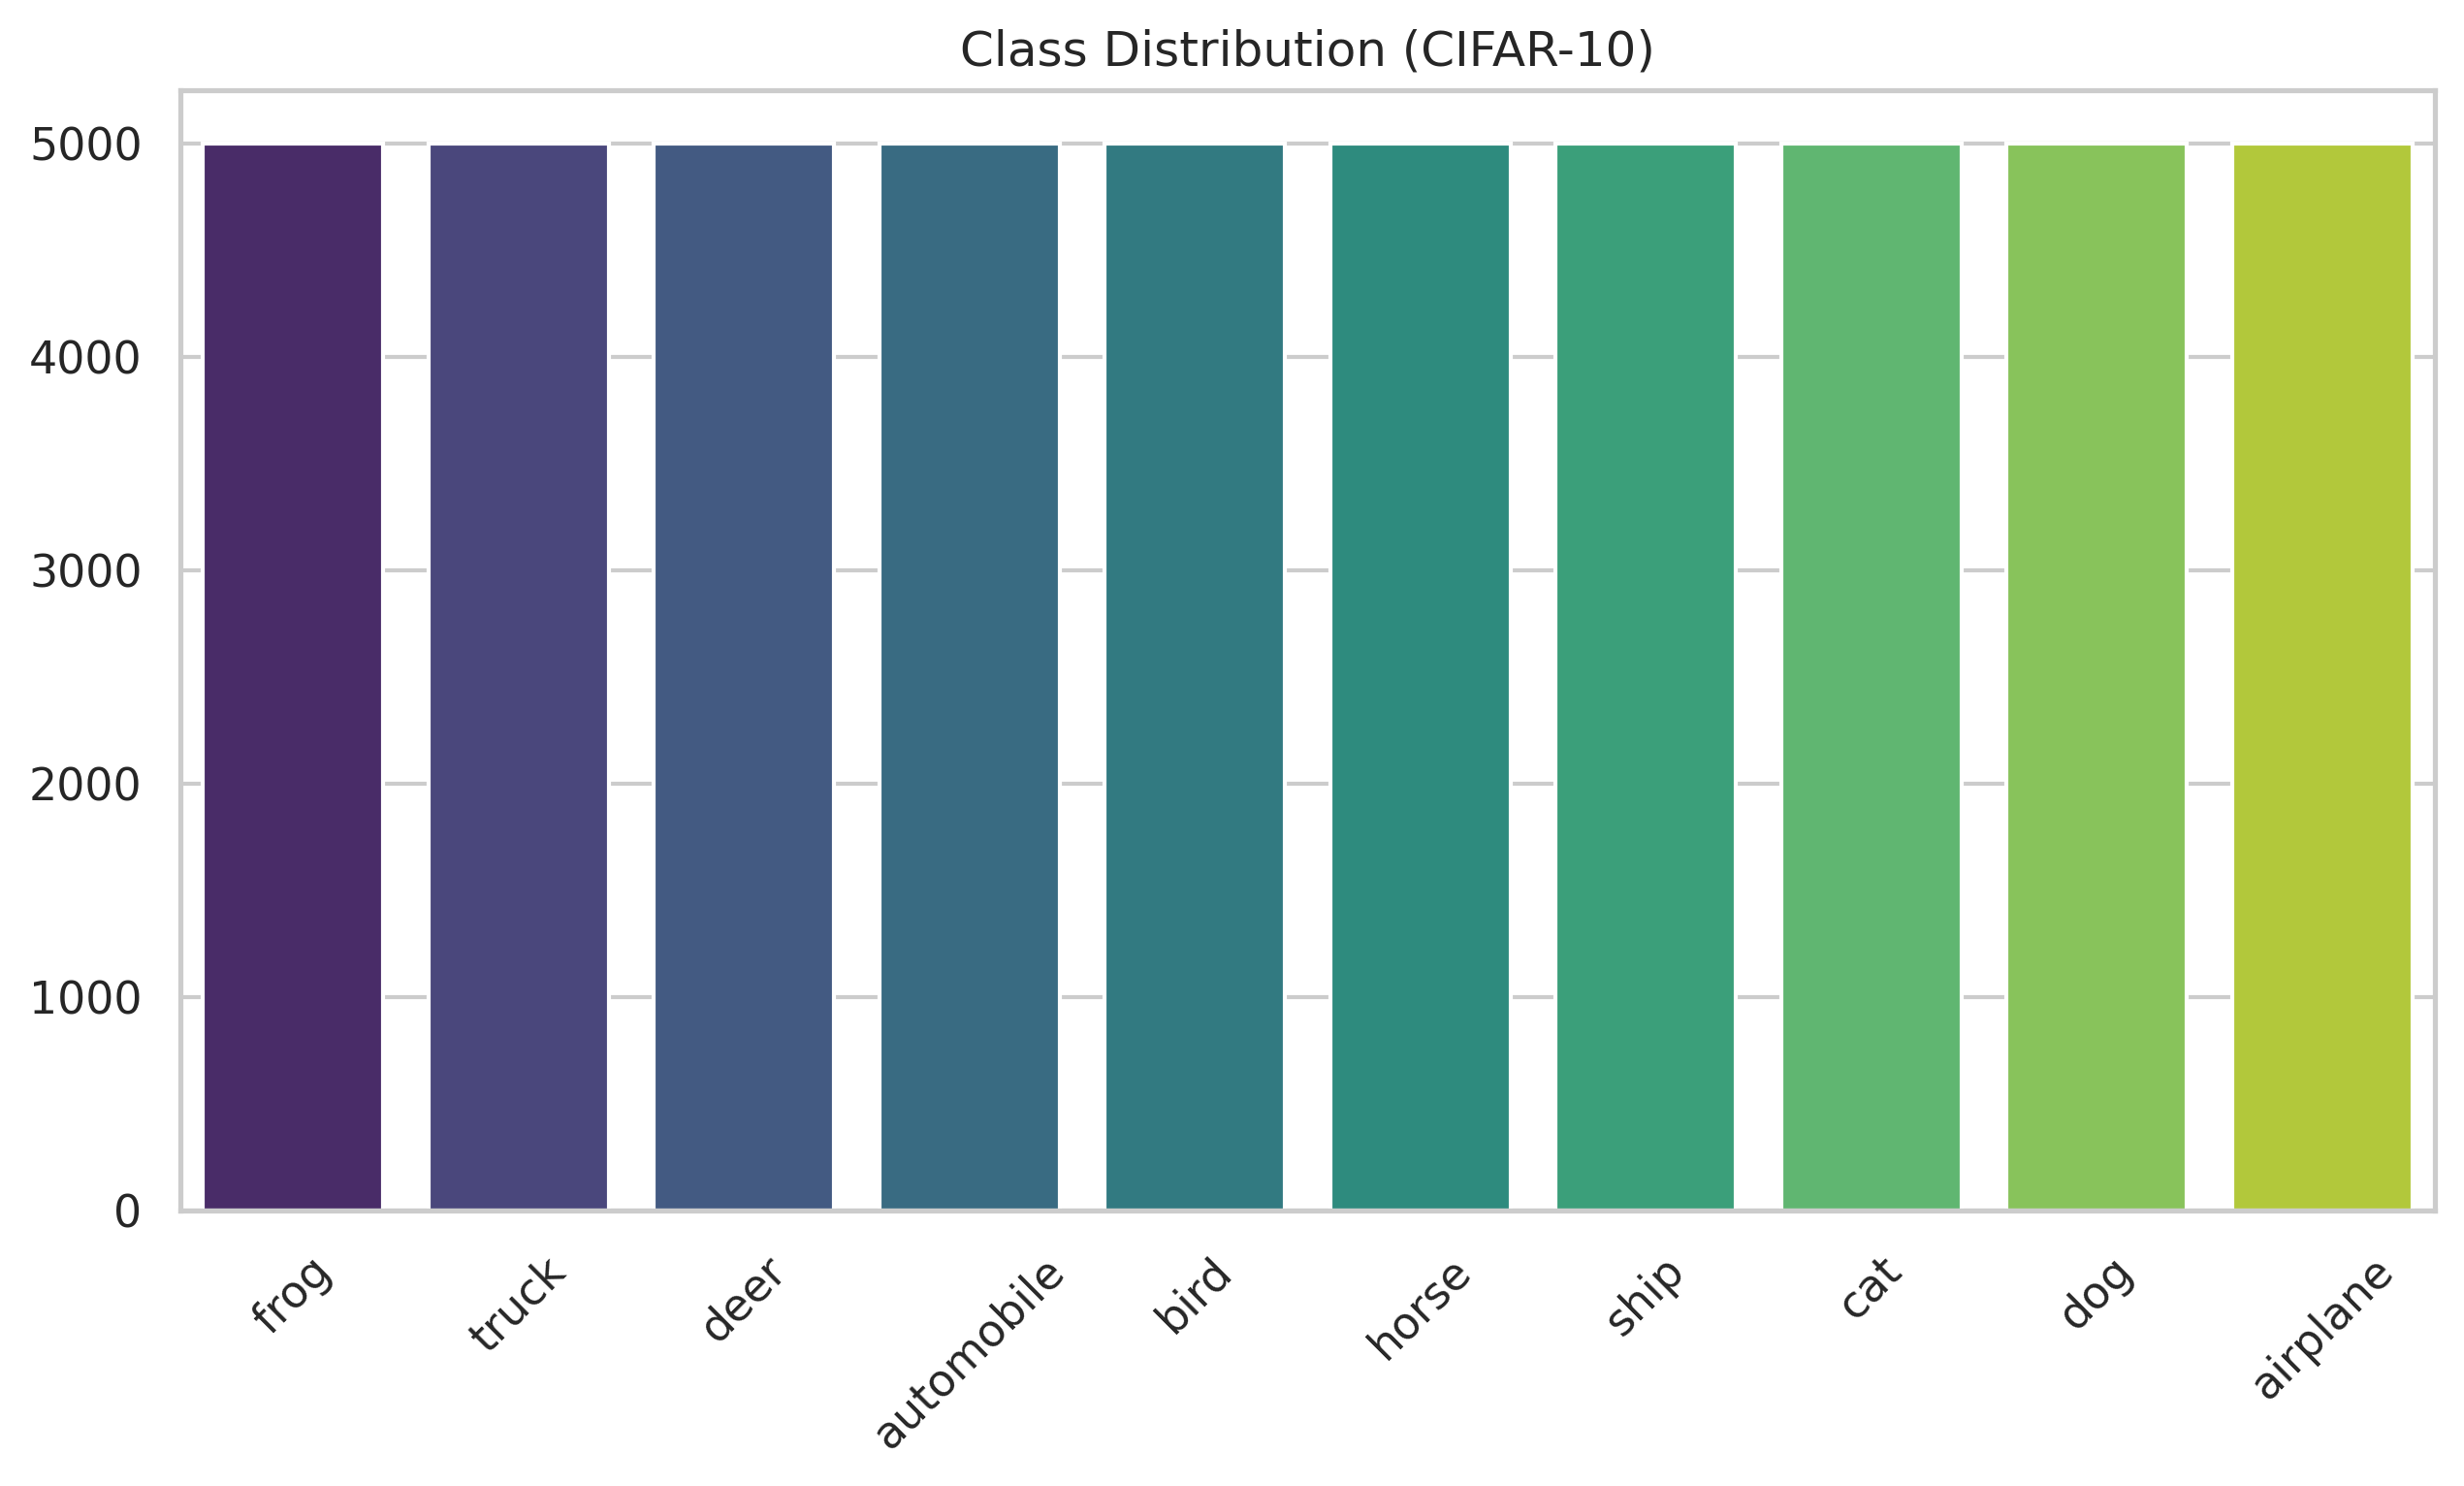
\includegraphics[width=0.80\textwidth]{images/cifar_class_dist.png}
    \caption{\textbf{Figure IMG-2} --- Class distribution across the CIFAR-10 training set. All 10 classes contain exactly 5{,}000 images, confirming perfect balance.
    \textit{Code:} \texttt{np.unique(labels, return\_counts=True)} then \texttt{plt.bar()}.}
    \label{fig:cifar_dist}
\end{figure}

\subsection{Statistical Analysis of Pixels}

We computed per-channel pixel statistics over the full 50,000-image training set
to characterize the color properties of the data and to derive the normalization
parameters that would be applied in any subsequent model training pipeline.

\begin{table}[H]
\centering
\caption{CIFAR-10 Per-Channel Pixel Statistics (training set, $n = 50{,}000$)}
\begin{tabular}{lcc}
\hline
\textbf{Channel} & \textbf{Mean} & \textbf{Std Deviation} \\
\hline
Red   & $\sim$125.31 & $\sim$62.99 \\
Green & $\sim$122.95 & $\sim$61.90 \\
Blue  & $\sim$113.87 & $\sim$66.56 \\
\hline
\end{tabular}
\label{tab:cifar_stats}
\end{table}

Several observations follow directly from Table~\ref{tab:cifar_stats}:

\begin{itemize}
    \item \textbf{Warm color bias:} The Red and Green channel means (~125 and ~123
    respectively) are noticeably higher than the Blue channel mean (~114). This
    indicates that the dataset as a whole leans toward warmer tones — a natural
    consequence of the prevalence of outdoor daylight scenes (animals on grass,
    vehicles on roads, aircraft in sky) in the collection.
    \item \textbf{High variance across all channels:} Standard deviations of
    approximately 62--67 across all three channels (on a 0--255 scale) indicate
    very high diversity in brightness and contrast. This rules out any assumption of
    a narrow intensity distribution and confirms that normalization
    (e.g.\ dividing by 255 or applying Z-score per channel using the values above)
    is essential before feeding images into neural networks.
    \item \textbf{Normalization reference values:} The channel means and standard
    deviations computed here serve as the canonical per-channel normalization
    parameters for CIFAR-10, consistent with values widely reported in the
    literature for this dataset.
\end{itemize}

The RGB pixel intensity distribution in Figure IMG-3 below visualizes
these statistics across the full pixel population. The distributions are broad and
relatively flat, with no sharp peaks, which is consistent with the high standard
deviations observed and reflects the wide variety of scene types present in the
dataset.

\begin{figure}[H]
    \centering
    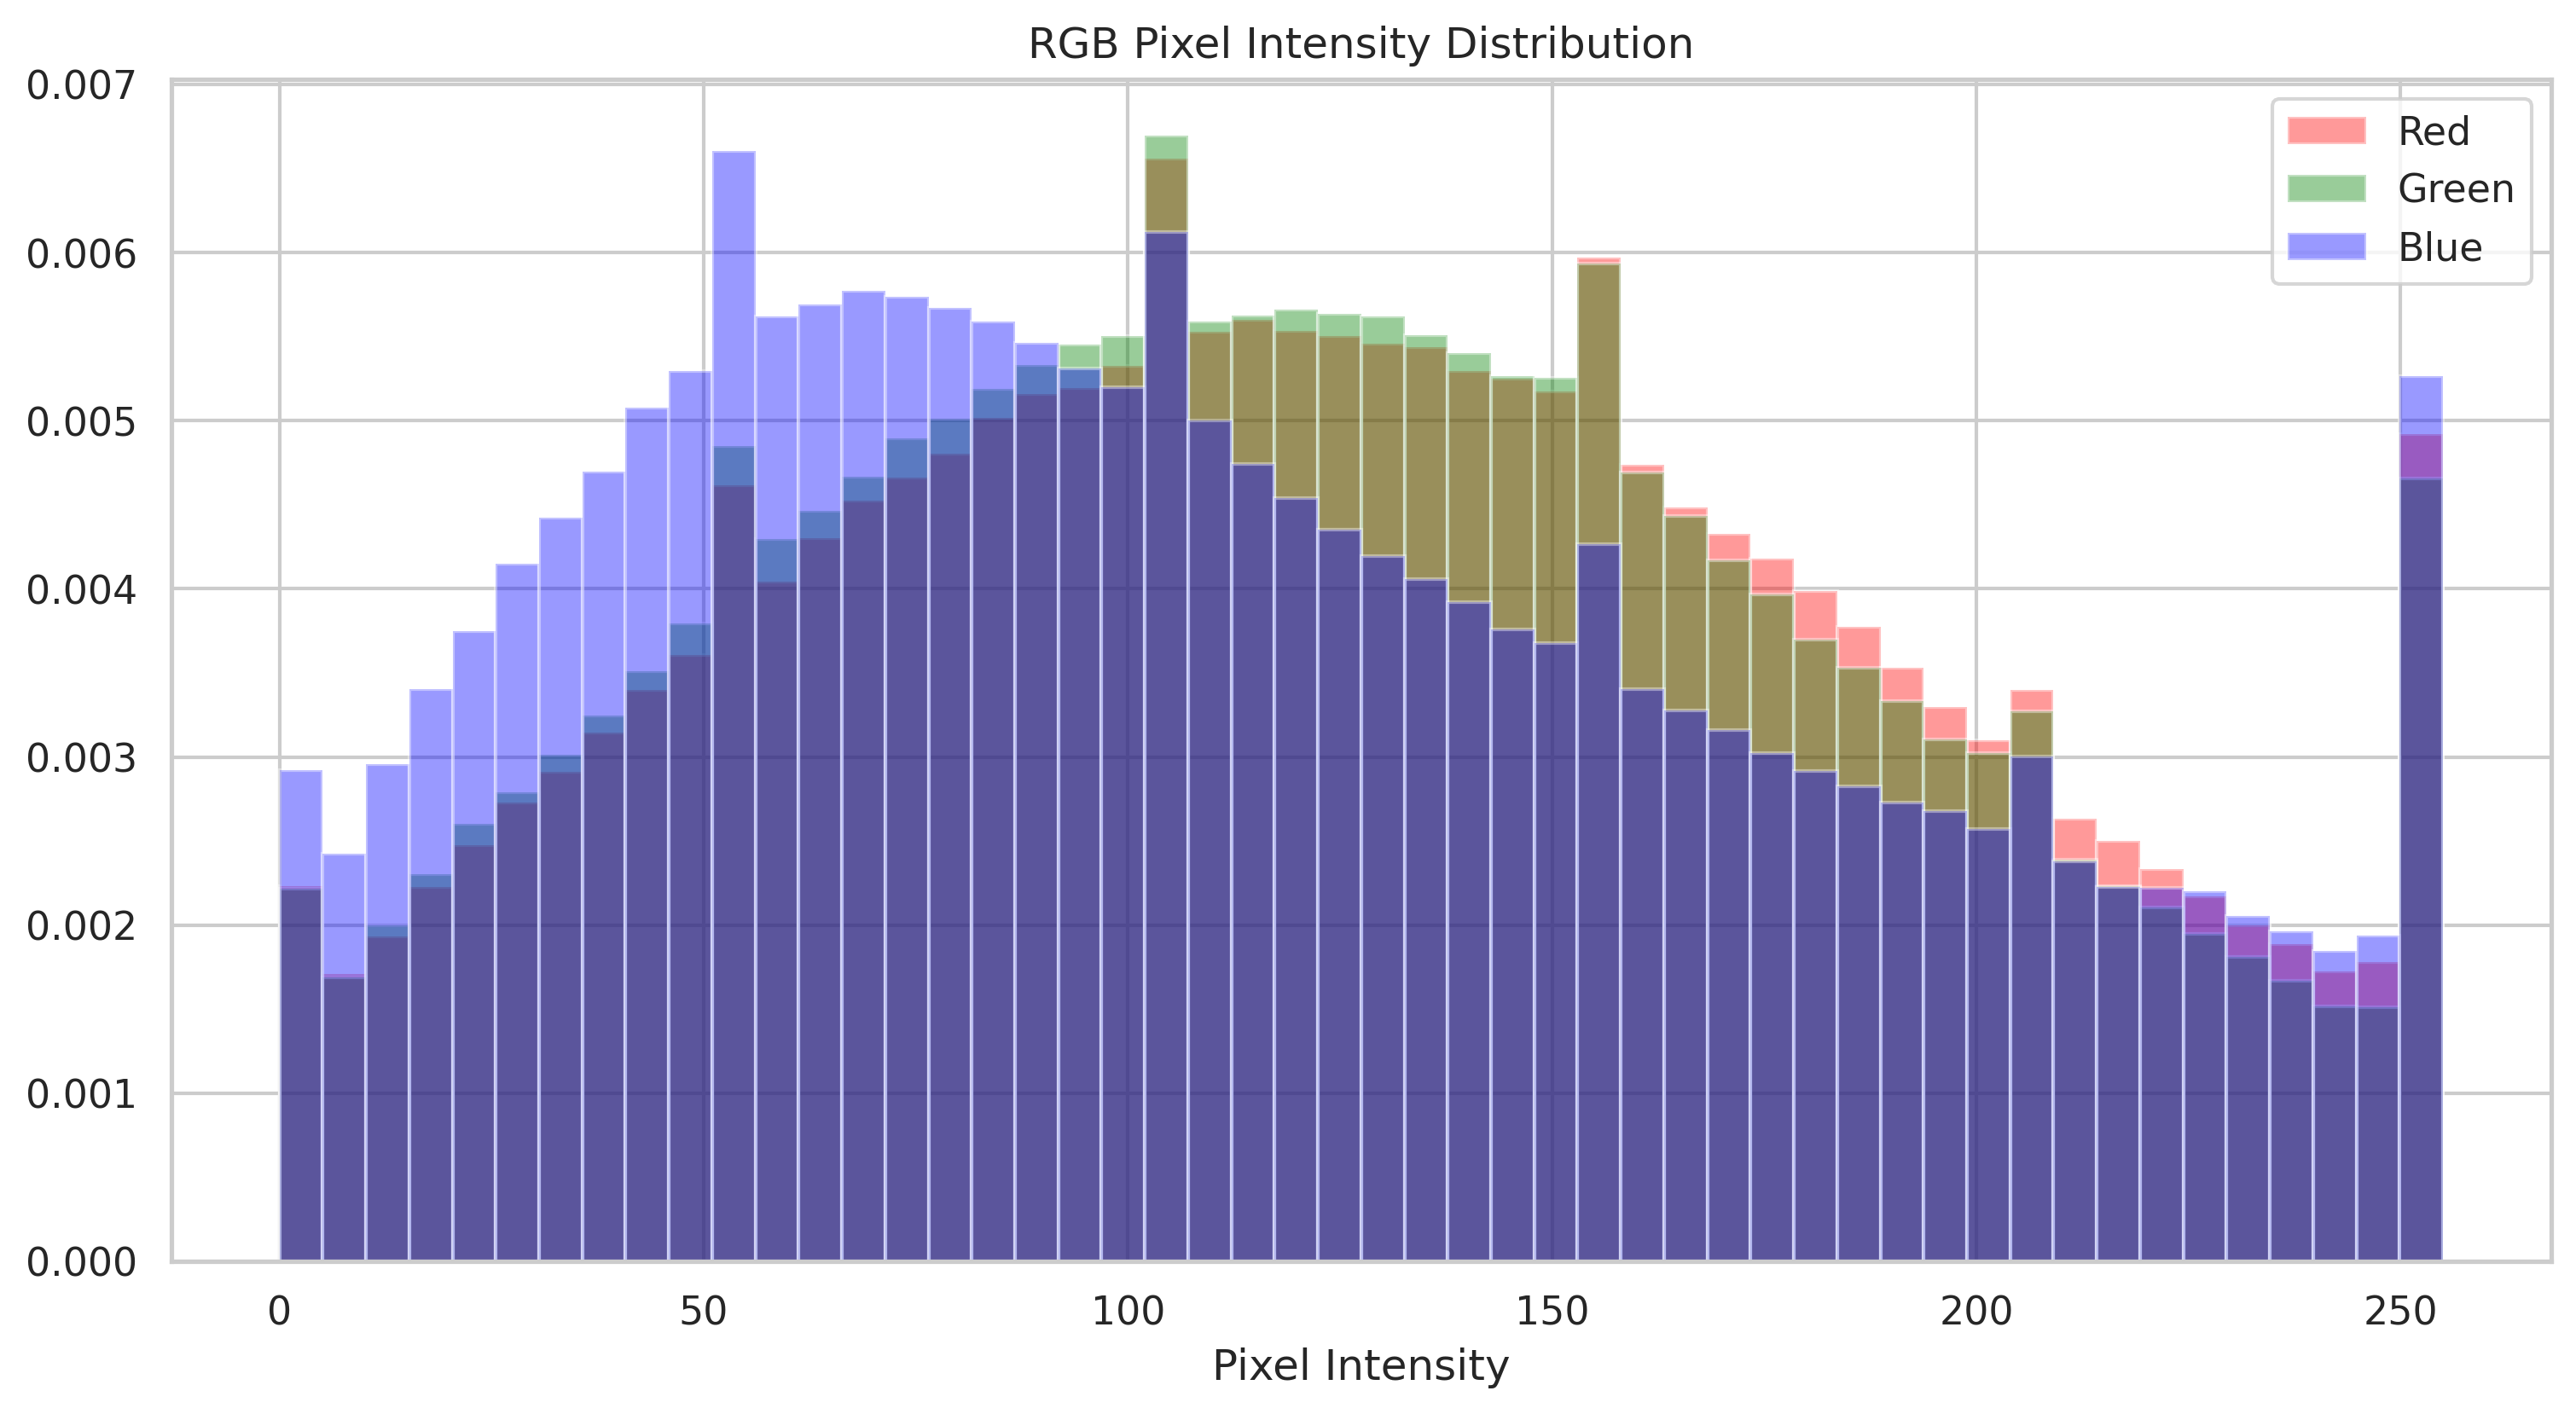
\includegraphics[width=0.85\textwidth]{images/cifar_rgb_dist.png}
    \caption{\textbf{Figure IMG-3} --- RGB channel intensity distributions across a sample of 5{,}000 CIFAR-10 training images. The broad, overlapping distributions reflect high photometric diversity.
    \textit{Code:} \texttt{images[:5000].reshape(-1, 3)} then \texttt{plt.hist()} per channel.}
    \label{fig:cifar_rgb}
\end{figure}

\subsection{Per-Class Visual Analysis}

To move beyond aggregate statistics, we examined the visual characteristics of
each class individually through two complementary techniques.

\subsubsection*{Mean Image per Class}

For each of the 10 classes, we computed the pixel-wise mean across all 5,000
member images (Figure IMG-4 below). The resulting ``average image'' reveals
the dominant spatial structure and color palette that is characteristic of each
category:

\begin{itemize}
    \item \textbf{Structured classes} such as \texttt{airplane} and \texttt{ship}
    produce mean images with discernible shapes — a central bright mass against
    a blue-toned background — suggesting that images within these classes share
    consistent spatial composition (subject centered, sky or water as background).
    \item \textbf{Animal classes} such as \texttt{cat}, \texttt{dog}, and
    \texttt{bird} produce heavily blurred mean images with no clear structure,
    indicating high intra-class variability in pose, viewpoint, and background.
    \item \textbf{Vehicle classes} (\texttt{automobile}, \texttt{truck}) show
    a warm central mass, reflecting consistent foreground object placement but
    variable background color.
\end{itemize}

This analysis suggests that models trained on CIFAR-10 will find vehicle and
aircraft classes easier to separate than animal classes, which show substantially
higher within-class variance.

\begin{figure}[H]
    \centering
    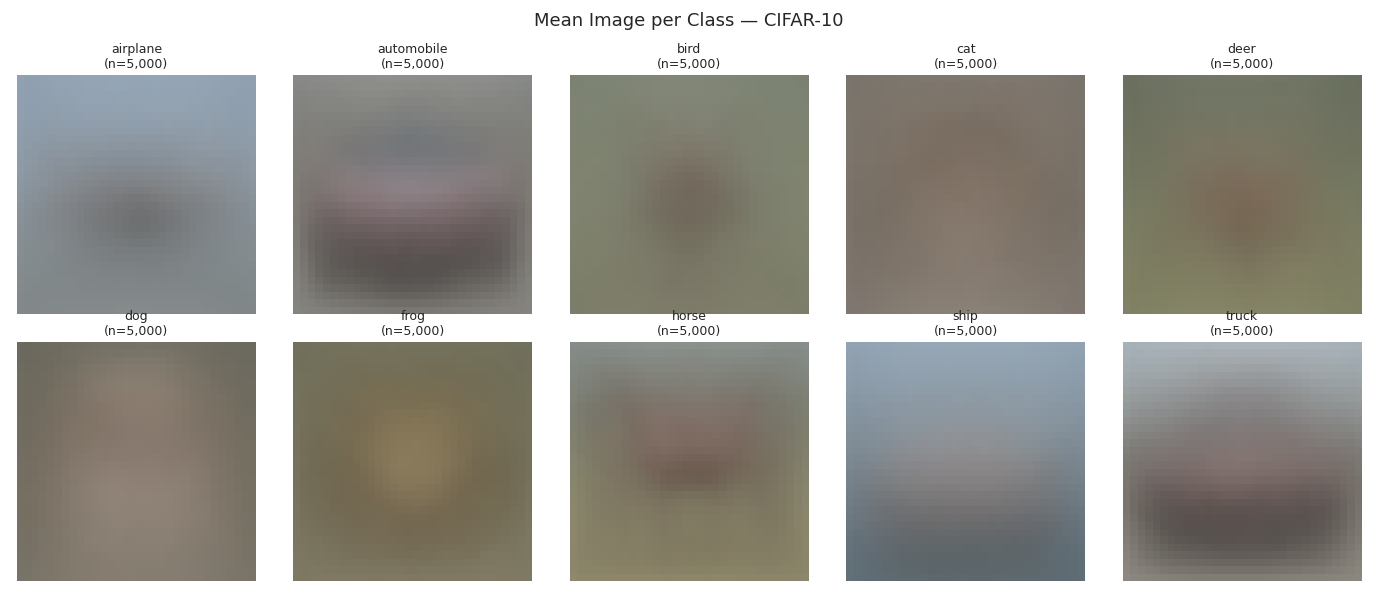
\includegraphics[width=0.95\textwidth]{images/cifar_mean_images.png}
    \caption{\textbf{Figure IMG-4} --- Pixel-wise mean image per class, computed over all 5{,}000 training images per category. Structured classes (airplane, ship) retain visible spatial patterns; animal classes blur into near-uniform patches.
    \textit{Code:} \texttt{images[labels==c].mean(axis=0).astype(np.uint8)} for each class \texttt{c}.}
    \label{fig:cifar_mean}
\end{figure}

\subsubsection*{Mean Brightness per Class}

Figure IMG-5 below shows the mean pixel brightness (averaged across
all three RGB channels and all pixels) for each class. This metric is a simple
but revealing indicator of the dominant scene context per category:

\begin{itemize}
    \item Classes with bright backgrounds such as \texttt{airplane} (sky),
    \texttt{ship} (sea or sky), and \texttt{automobile} (road, daylight) tend
    to register higher mean brightness values.
    \item Darker classes such as \texttt{frog} and \texttt{deer} typically
    appear against vegetation or shaded environments, pulling their mean
    brightness lower.
\end{itemize}

The variation in brightness across classes is a useful signal: a model that
learns to associate brightness with certain class priors is leveraging a real
statistical property of the data, not an artifact.

\begin{figure}[H]
    \centering
    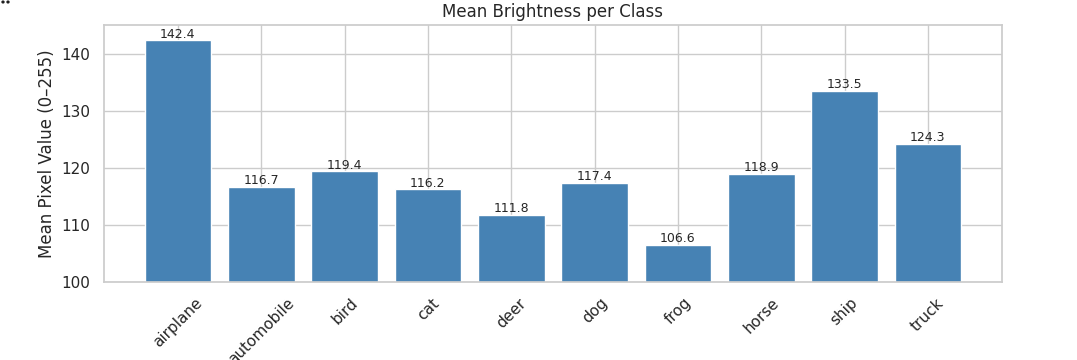
\includegraphics[width=0.85\textwidth]{images/cifar_brightness.png}
    \caption{\textbf{Figure IMG-5} --- Mean pixel brightness per class. Classes in bright outdoor environments (airplane, ship) score higher; nature-heavy classes (frog, deer) score lower.
    \textit{Code:} \texttt{images[labels==c].mean()} per class, then \texttt{plt.bar()}.}
    \label{fig:cifar_bright}
\end{figure}

\subsection{Data Quality Check}

Before proceeding to any modelling steps, we performed a rigorous data integrity
audit of the full 50,000-image training set. Each check targets a specific failure
mode that could silently corrupt model training if left undetected.

\begin{table}[H]
\centering
\caption{CIFAR-10 Data Quality Audit Results}
\begin{tabular}{lcc}
\hline
\textbf{Check} & \textbf{Method} & \textbf{Result} \\
\hline
Missing / NaN pixel values   & \texttt{np.isnan()} over full array & 0 \\
All-zero images              & Row-wise min check                  & 0 \\
Constant-value images        & Row-wise unique value check         & 0 \\
Exact duplicate images       & MD5 hash per image                  & 0 \\
Label range integrity        & \texttt{np.unique(labels)}          & OK — $[0, 9]$ \\
Number of distinct classes   & Count of unique label values        & 10 / 10 \\
\hline
\end{tabular}
\label{tab:cifar_quality}
\end{table}

All six checks passed with zero anomalies detected, as summarized visually in
Figure IMG-6 below. This is expected for a professionally curated
benchmark dataset, but confirming it explicitly is still good practice — it
rules out any corruption introduced during download, decompression, or loading
via the \texttt{tensorflow.keras.datasets} API. The conclusion is that no
cleaning, deduplication, or label correction is required prior to model training.

\begin{figure}[H]
    \centering
    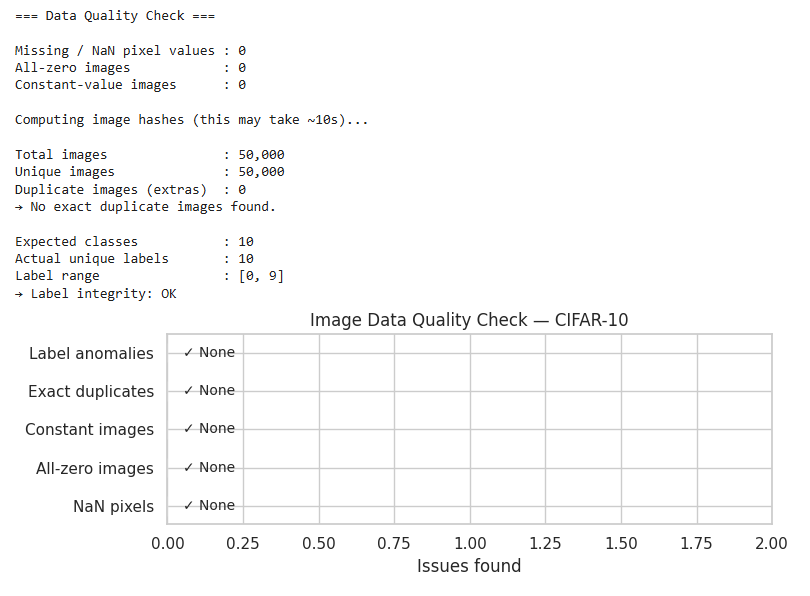
\includegraphics[width=0.75\textwidth]{images/cifar_quality_check.png}
    \caption{\textbf{Figure IMG-6} --- Data quality audit summary for CIFAR-10. All six checks return zero anomalies.
    \textit{Code:} \texttt{np.isnan(images.astype(float)).sum()}, MD5 hash deduplication, \texttt{np.unique(labels)}, etc.}
    \label{fig:cifar_quality}
\end{figure}

\subsection{Key Findings and Preprocessing Recommendations}

\begin{importantbox}
\textbf{Summary of Image EDA Key Findings:}
\begin{itemize}
    \item \textbf{Perfect class balance:} Exactly 5{,}000 images per class. No resampling (SMOTE, oversampling) required --- standard cross-entropy loss is directly applicable.
    \item \textbf{Warm colour bias:} Red ($\sim$125) and Green ($\sim$123) channel means exceed Blue ($\sim$114), reflecting the prevalence of outdoor daylight scenes (animals on grass, vehicles on roads, aircraft against sky).
    \item \textbf{High photometric variance:} Std.\ deviations of 62--67 across all channels confirm that per-channel Z-score normalisation (using the computed means and stds) is strongly recommended before model training.
    \item \textbf{Intra-class variability:} Animal classes (\texttt{cat}, \texttt{dog}, \texttt{bird}) show highly blurred mean images, indicating extreme pose and background variation. \textbf{Data augmentation} (random horizontal flip, random crop, colour jitter) will be particularly beneficial for these categories.
    \item \textbf{Structured vs.\ unstructured classes:} \texttt{airplane} and \texttt{ship} retain clear spatial patterns in mean images (subject centred against uniform background), suggesting models will find these classes easier to separate.
    \item \textbf{Data integrity:} 6/6 quality checks passed --- zero NaN pixels, zero all-zero images, zero duplicate images, valid label range $[0, 9]$, all 10 classes present.
    \item \textbf{No resize needed:} All images are uniformly $32\times32$ px --- no spatial preprocessing required.
    \item \textbf{Recommended normalisation:} \texttt{mean=[125.31, 122.95, 113.87] / 255}, \texttt{std=[62.99, 61.90, 66.56] / 255} (canonical CIFAR-10 values).
\end{itemize}
\end{importantbox}

% =======================================================================
\section{Exploratory Data Analysis: Multimodal Data}
\label{sec:multi}

\subsection{Dataset Overview}
For the multimodal modality, we explored the \textbf{Flickr8k Dataset}, a standard benchmark for image captioning tasks that pairs real-world photographs with descriptive natural language captions written by human annotators.

\begin{itemize}
    \item \textbf{Source:} \href{https://www.kaggle.com/datasets/adityajn105/flickr8k}{Flickr8k Dataset by Aditya Jain (Kaggle)} / \href{https://huggingface.co/datasets/nlphuji/flickr8k}{HuggingFace: \texttt{nlphuji/flickr8k}}
\end{itemize}

\begin{importantbox}
\textbf{Dataset Statistics:}
\begin{itemize}
    \item \textbf{Total Images:} 8{,}092 unique real-world photographs from Flickr.
    \item \textbf{Total Captions:} 40{,}460 (exactly \textbf{5 distinct human-annotated captions per image}).
    \item \textbf{Image Format:} JPEG, varying aspect ratios and resolutions (most longest-edge $= 500$ px).
    \item \textbf{Caption Format:} English free-text descriptions, lowercase, no standard punctuation.
    \item \textbf{Missing values:} 0 missing captions or image references --- perfect data integrity.
    \item \textbf{Task suitability:} Standard benchmark for \textbf{Image Captioning}, \textbf{Visual Question Answering}, and \textbf{Cross-modal Retrieval}.
\end{itemize}
\end{importantbox}

Flickr8k is distinct from the other datasets in this report because it requires \emph{jointly} understanding two fundamentally different data types --- pixels and language --- in alignment. No single modality-specific model is sufficient; successful approaches must bridge the \textbf{visual encoder} (e.g., CNN or ViT) and the \textbf{language decoder} (e.g., LSTM or Transformer).

\subsection{Image Modality Analysis}

\subsubsection*{Image Dimension Distribution}

Unlike CIFAR-10, Flickr8k images do not have a uniform resolution. Figure MM-1 below shows the scatter of image widths and heights across the dataset.

\begin{figure}[H]
    \centering
    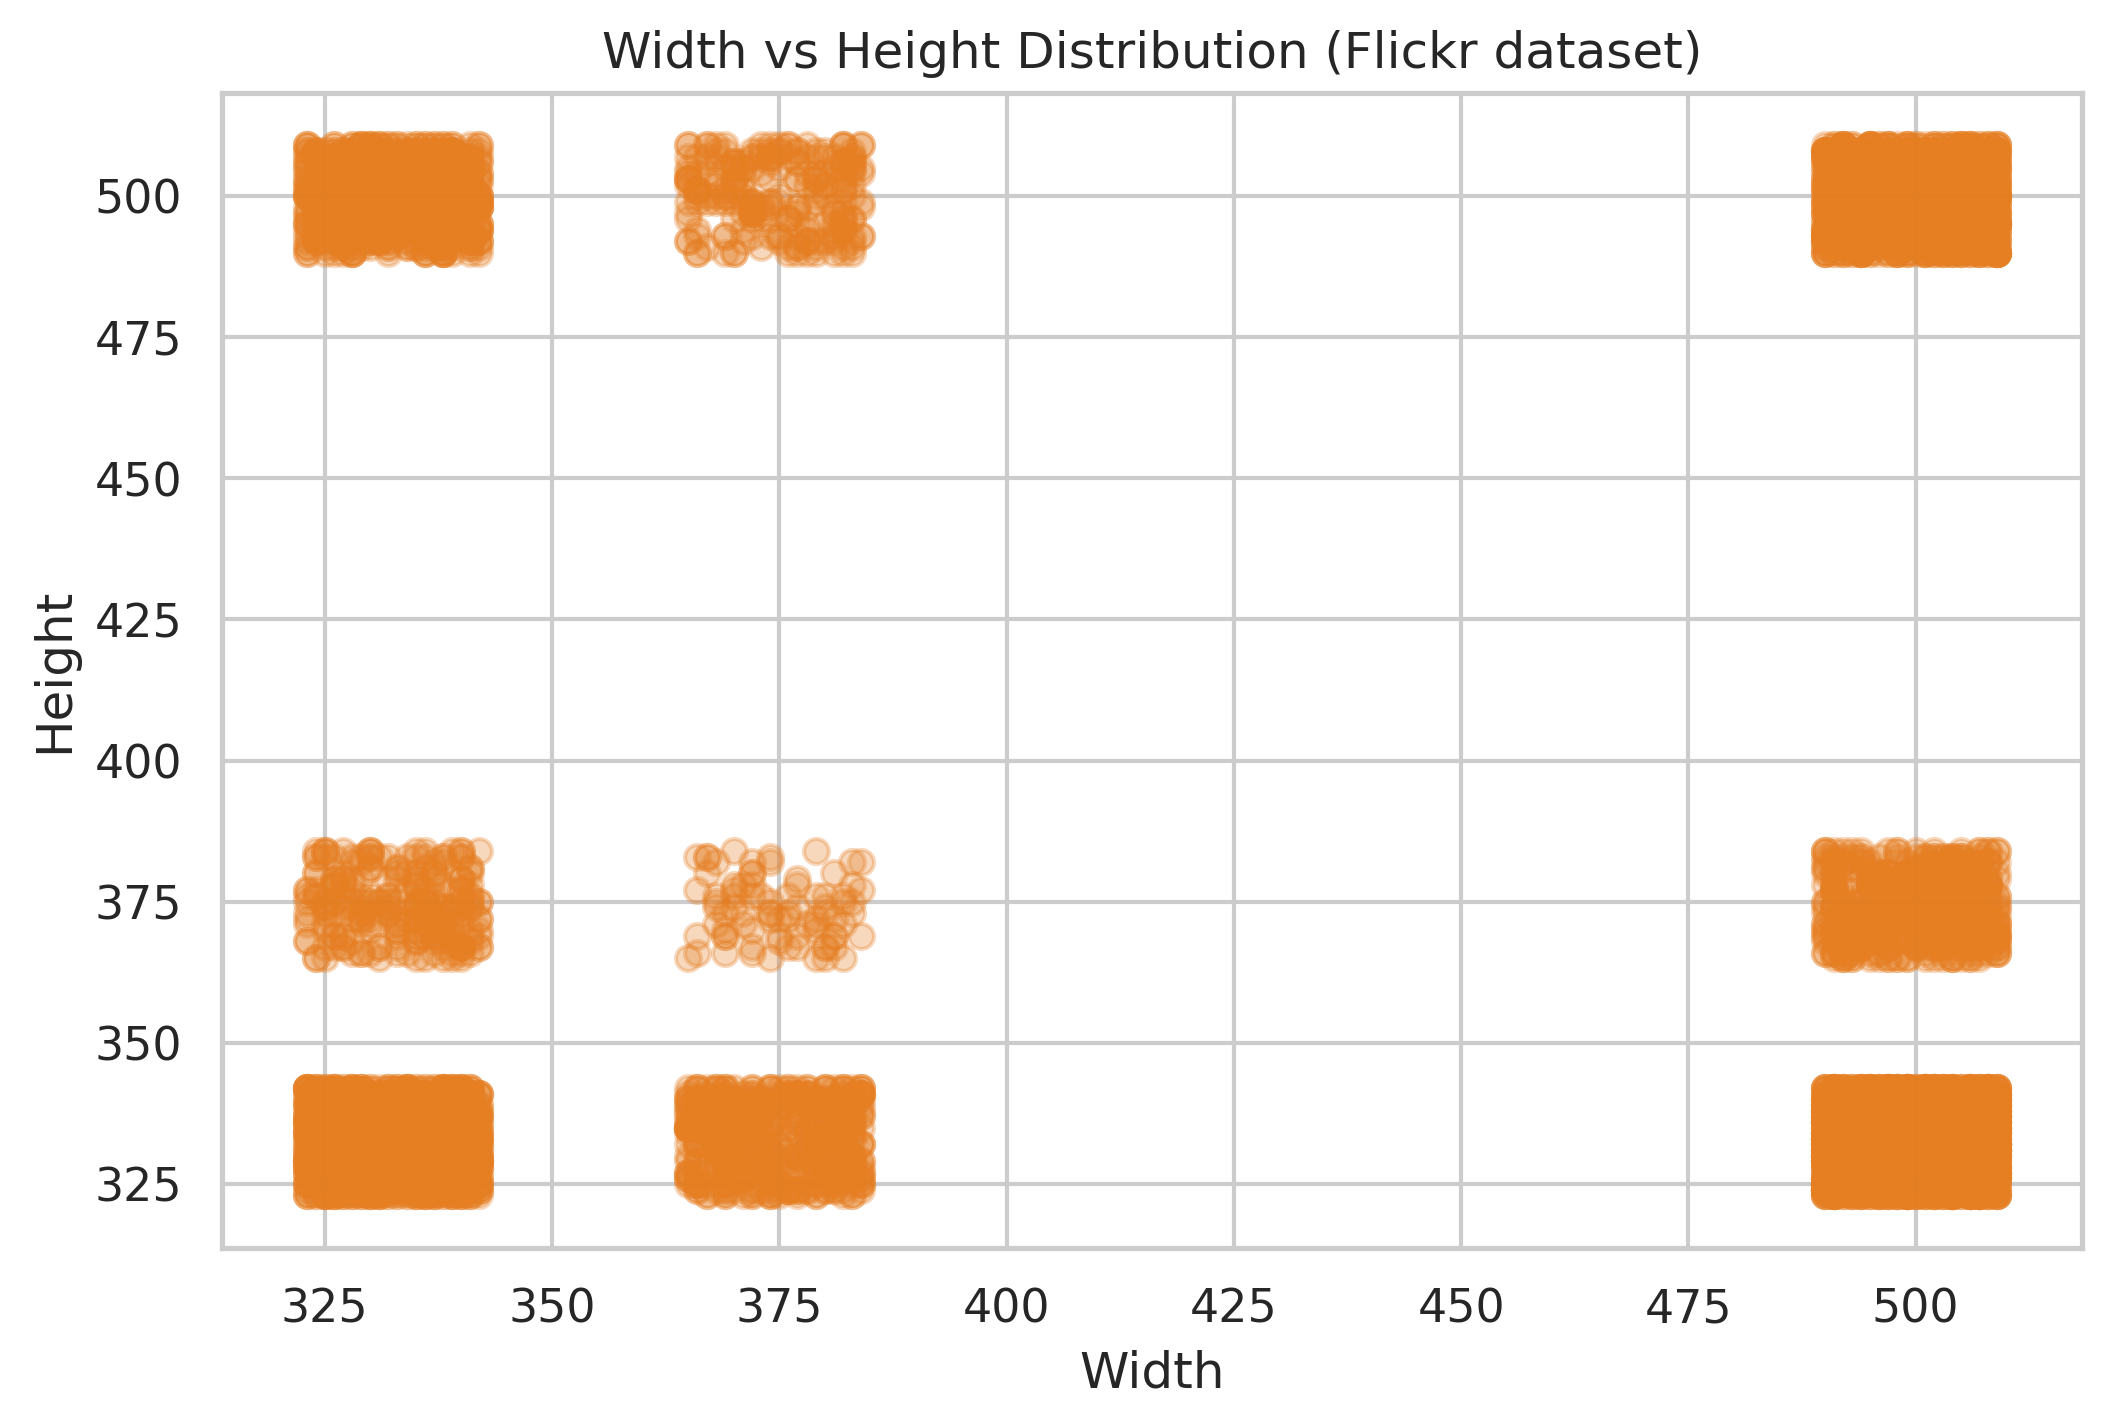
\includegraphics[width=0.75\textwidth]{images/multi_dimensions.png}
    \caption{\textbf{Figure MM-1} --- Image Width vs.\ Height Distribution across 8{,}092 Flickr8k images. Two dominant clusters appear: landscape orientation (width $>$ height) and portrait orientation (height $>$ width). Most images have their longest edge at 500 px.
    \textit{Code:} \texttt{PIL.Image.open(img).size} iterated over the dataset, then \texttt{plt.scatter(widths, heights)}.}
    \label{fig:multi_dims}
\end{figure}

Key observations:
\begin{itemize}
    \item Images cluster into two dominant groups: \textbf{landscape} (e.g., $500 \times 333$) and \textbf{portrait} (e.g., $375 \times 500$), with the landscape orientation being more common.
    \item No images are square or extremely narrow, which is consistent with consumer photography.
    \item \textbf{Preprocessing required:} All images must be resized (e.g., to $224 \times 224$ for ResNet/ViT) with aspect-ratio-preserving padding or center-cropping before model ingestion.
\end{itemize}

\subsubsection*{RGB Channel Pixel Distributions}

Figure MM-2 below plots the per-channel pixel intensity histograms for a sample of 500 images. Comparing this to CIFAR-10 reveals several differences:

\begin{figure}[H]
    \centering
    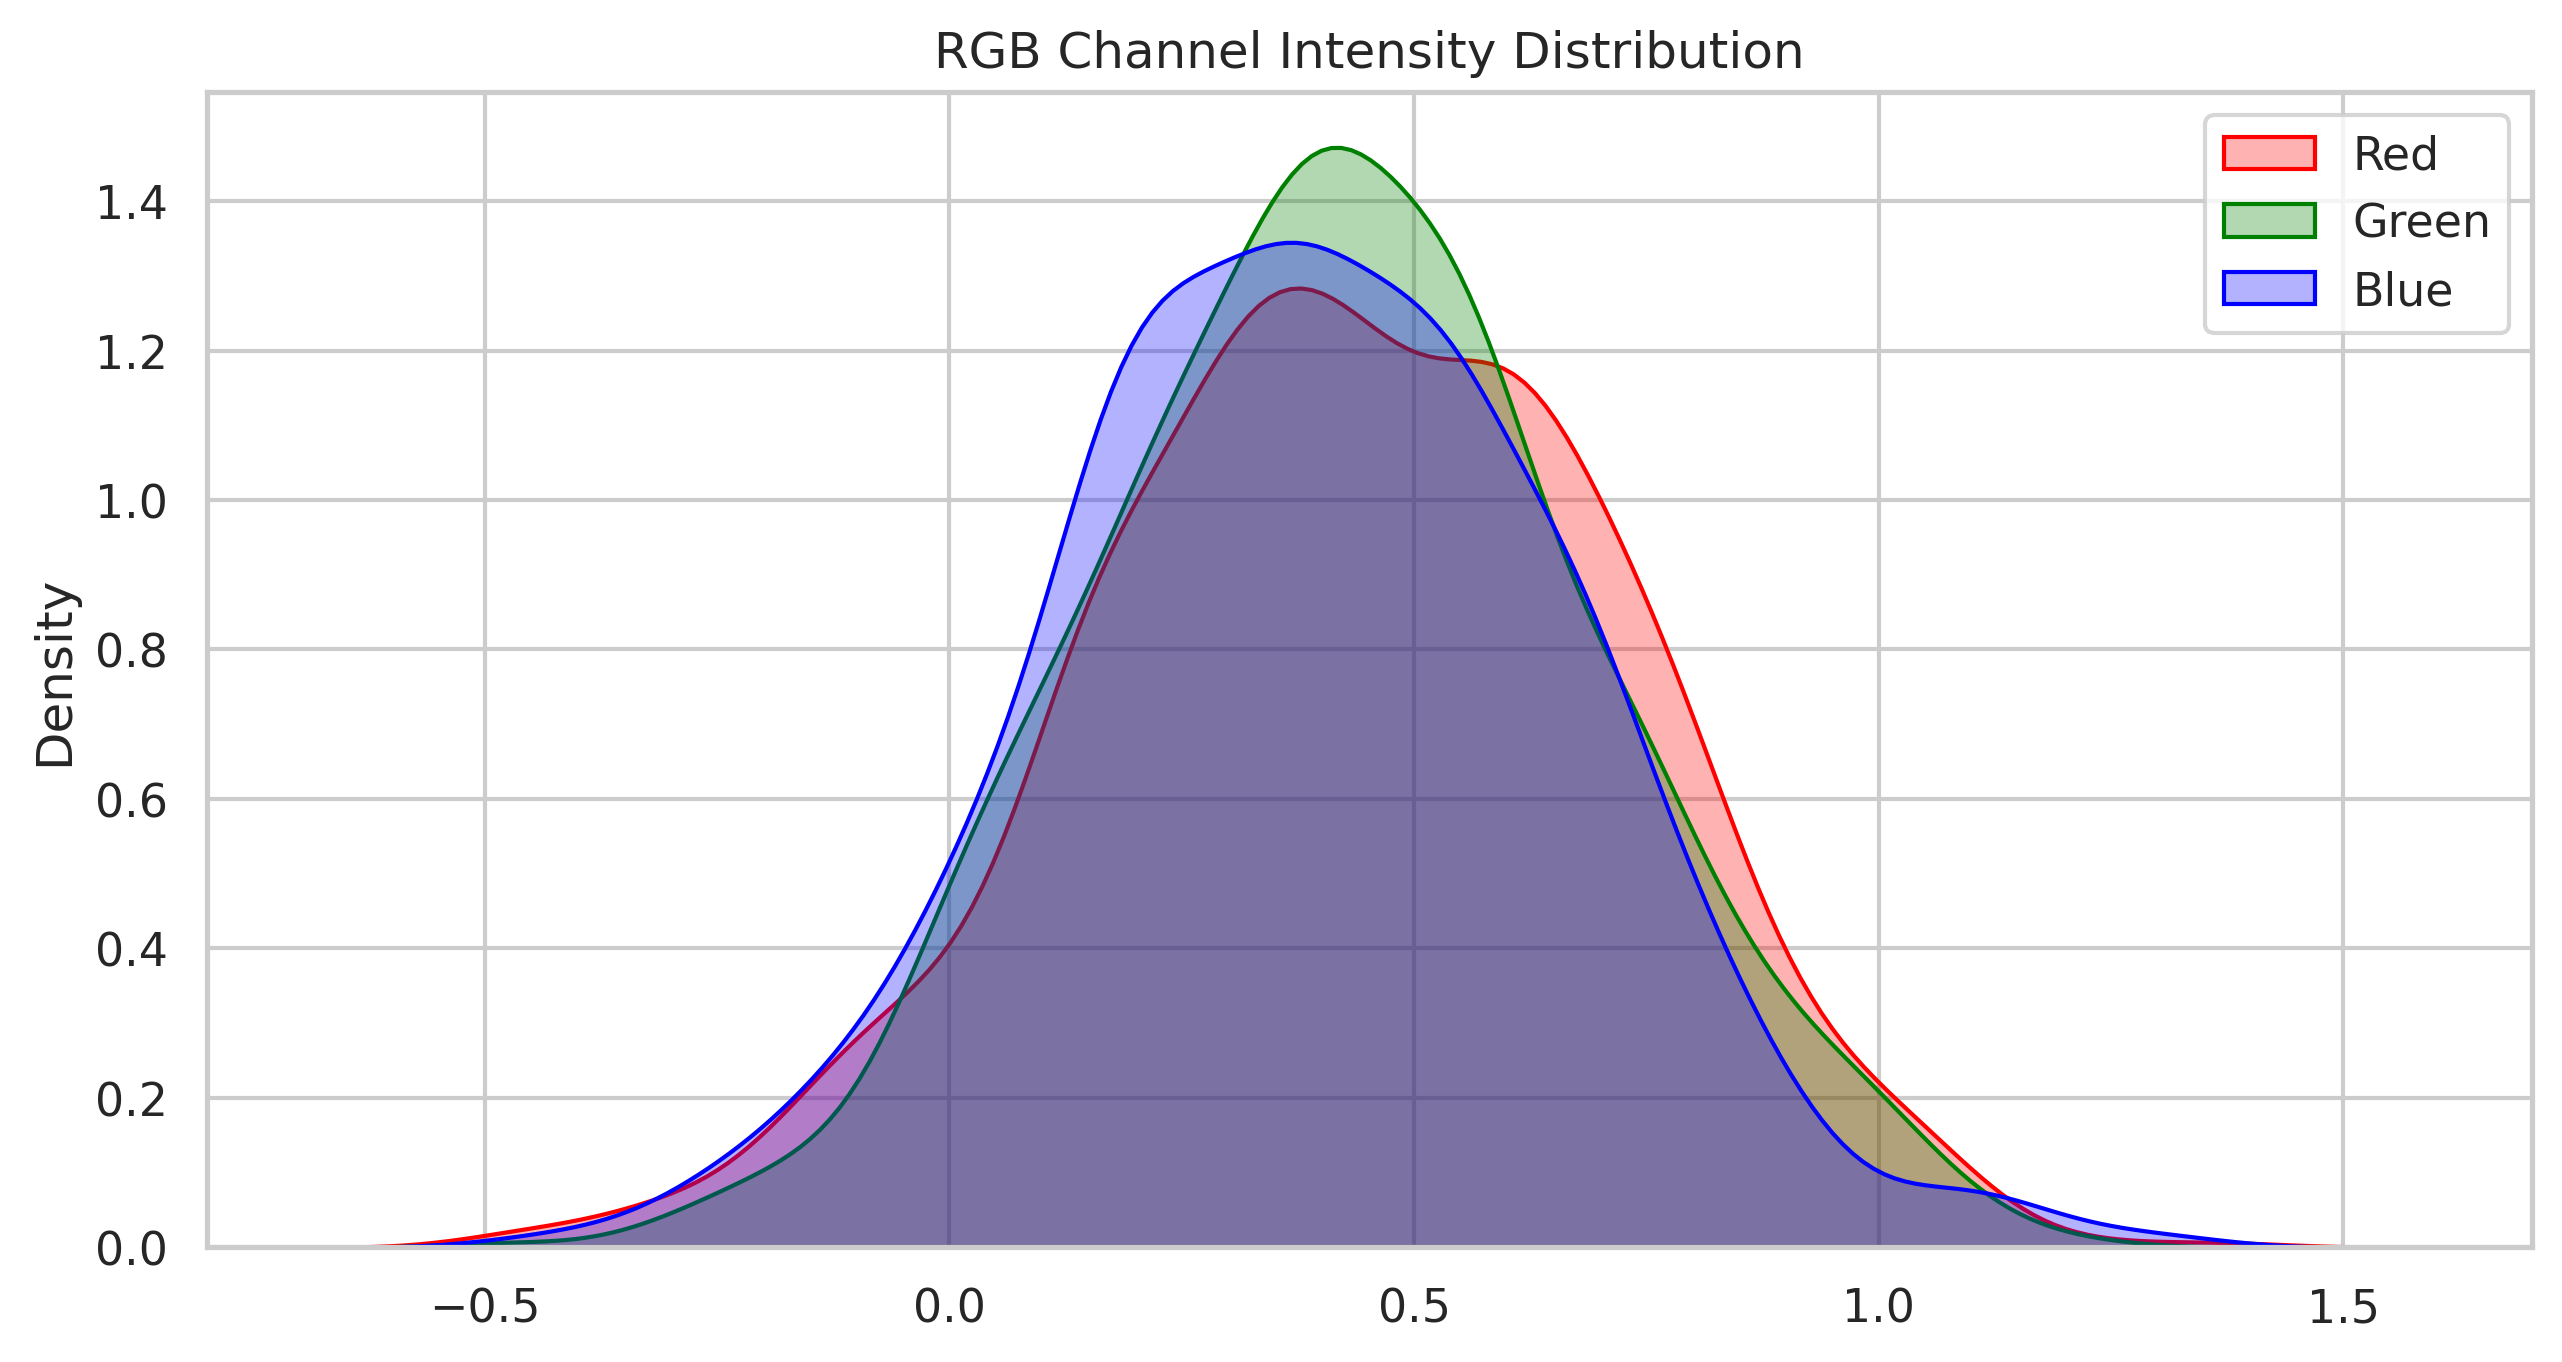
\includegraphics[width=0.85\textwidth]{images/multi_rgb_dist.png}
    \caption{\textbf{Figure MM-2} --- RGB Channel Pixel Intensity Distributions for a 500-image sample from Flickr8k.
    \textit{Code:} \texttt{np.array(img).reshape(-1, 3)} for each image, then \texttt{plt.hist(channel\_values, bins=50)} per channel.}
    \label{fig:multi_rgb}
\end{figure}

\begin{itemize}
    \item \textbf{Broader, more multi-modal distributions:} Unlike CIFAR-10's relatively flat distributions, Flickr8k shows peaks at both the low end (dark scenes, shadows) and high end (bright skies, reflective surfaces), reflecting the much greater photometric diversity of real-world photography.
    \item \textbf{Warm bias persists:} The Red channel tends to have a slightly higher mean than Blue, consistent with natural outdoor photography.
    \item \textbf{Normalization reference:} ImageNet mean/std normalization (\texttt{mean=[0.485, 0.456, 0.406], std=[0.229, 0.224, 0.225]}) is appropriate for this dataset when using pre-trained models.
\end{itemize}

\subsection{Text Modality Analysis}

\subsubsection*{Caption Length Distribution (Character Level)}

Figure MM-3 below shows a box plot of caption lengths in characters (all captions pooled). This provides a first look at the distribution of caption verbosity.

\begin{figure}[H]
    \centering
    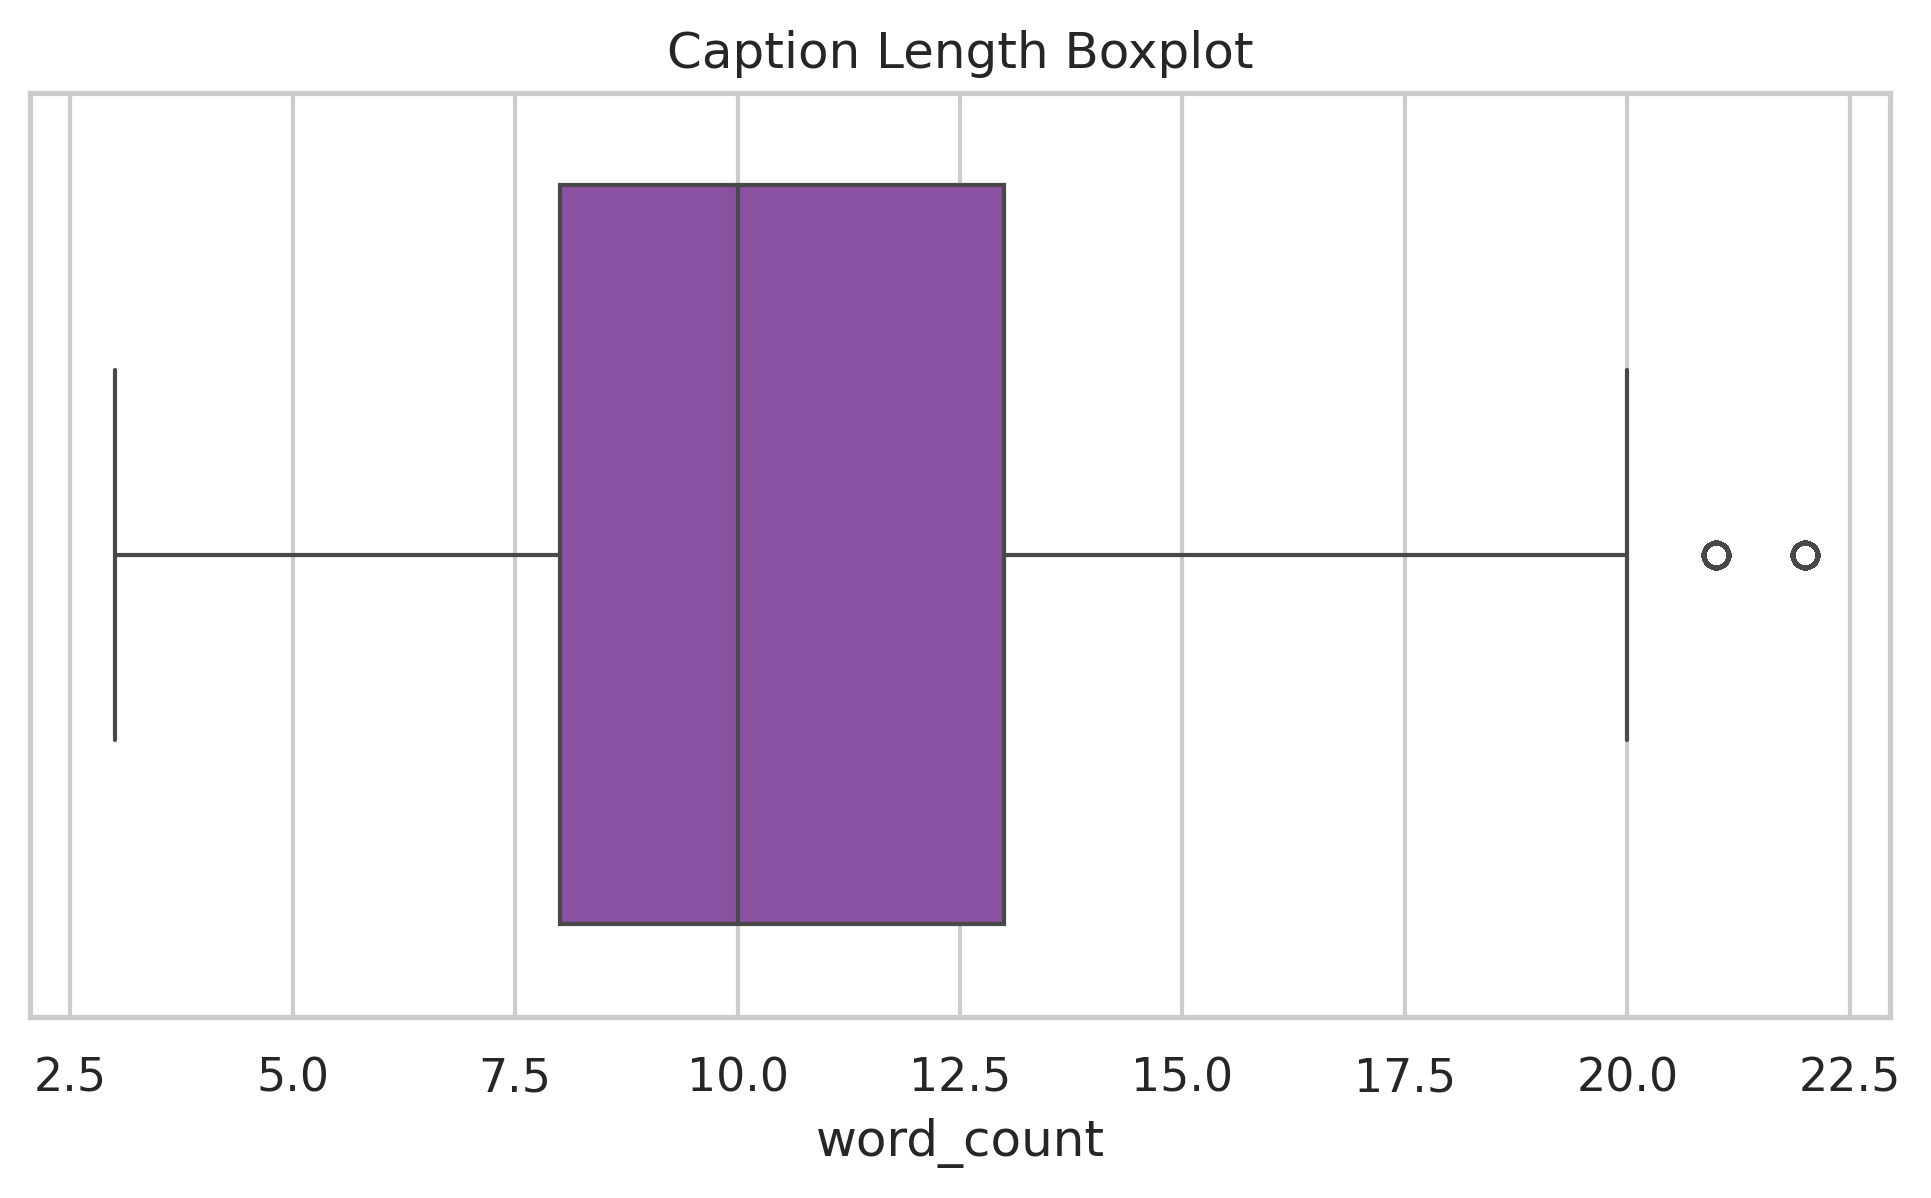
\includegraphics[width=0.65\textwidth]{images/multi_caption_box.png}
    \caption{\textbf{Figure MM-3} --- Caption Character Length --- Box Plot for all 40{,}460 captions in Flickr8k.
    \textit{Code:} \texttt{df['cap\_len'] = df['caption'].apply(len)}, then \texttt{plt.boxplot()}.}
    \label{fig:multi_cap_box}
\end{figure}

\begin{itemize}
    \item The interquartile range is compact, indicating consistent caption lengths across annotators.
    \item Few extreme outliers exist at both ends --- annotators consistently produced moderate-length descriptions.
\end{itemize}

\subsubsection*{Caption Word Count Distribution}

Figure MM-4 below breaks caption length down to word (token) count. This is the operationally relevant metric for sequence modelling.

\begin{figure}[H]
    \centering
    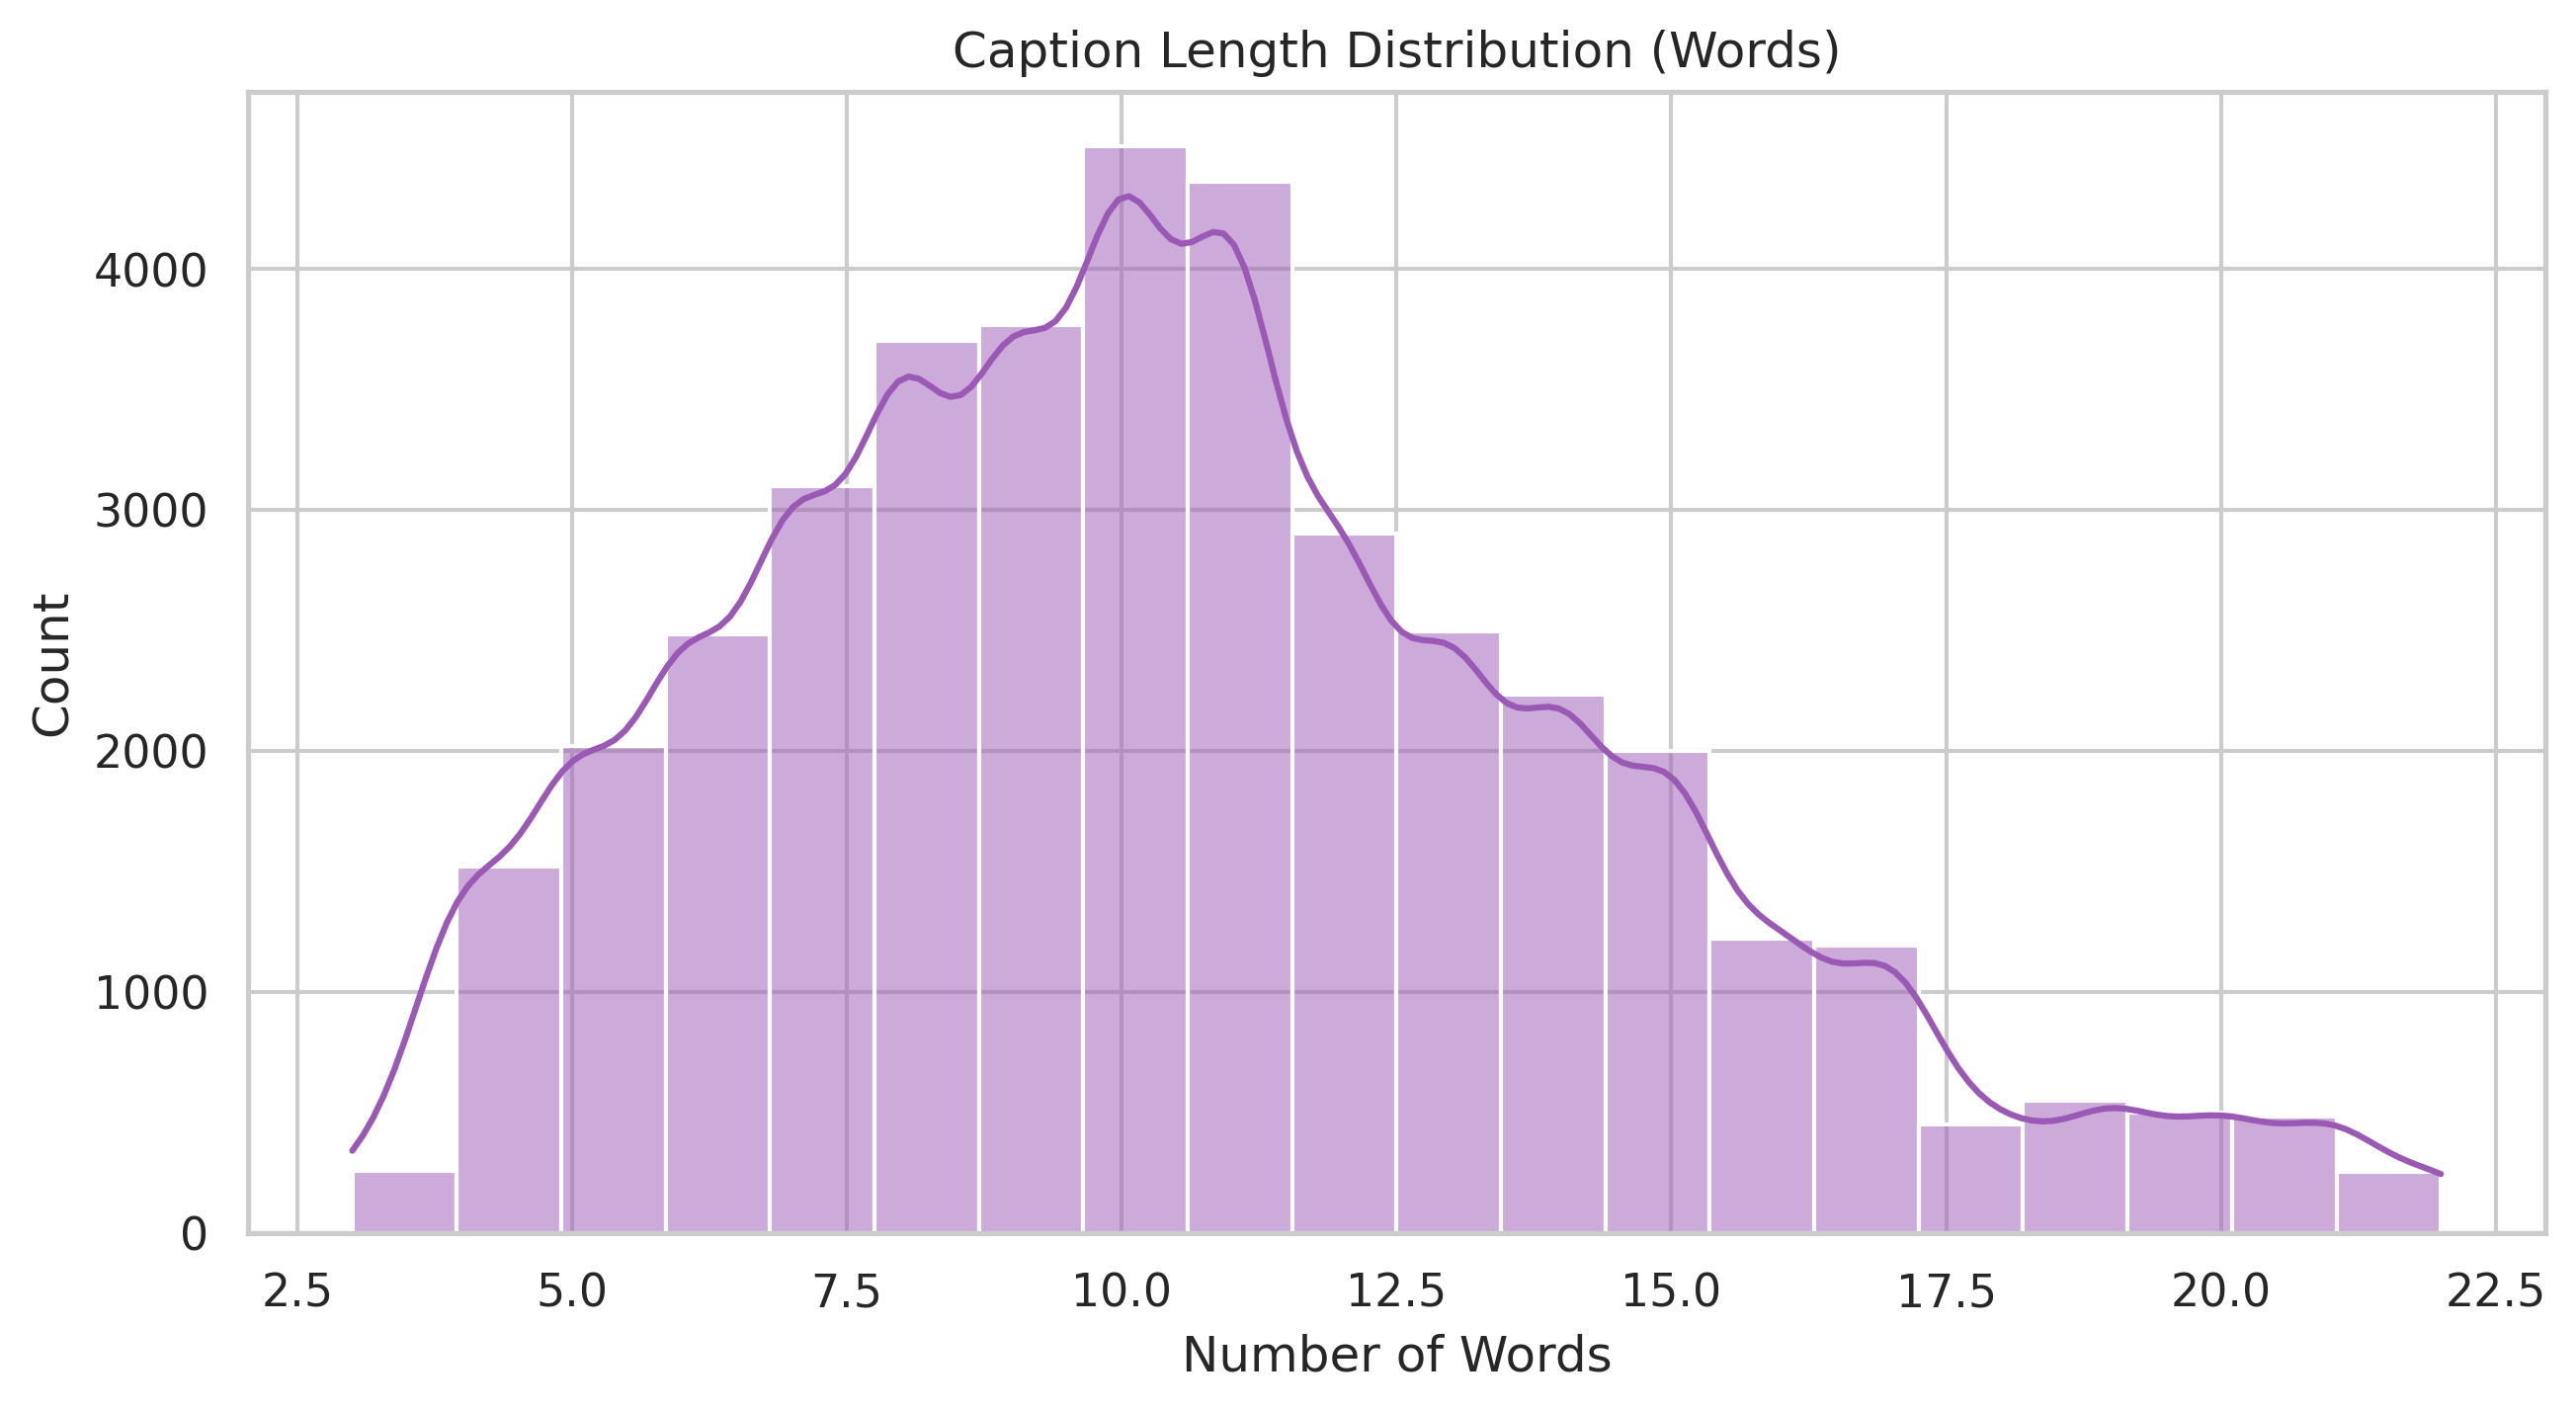
\includegraphics[width=0.80\textwidth]{images/multi_caption_len.png}
    \caption{\textbf{Figure MM-4} --- Caption Word Count Distribution across 40{,}460 captions. The distribution is unimodal and approximately normal, peaking at 10--11 words.
    \textit{Code:} \texttt{df['n\_words'] = df['caption'].str.split().str.len()}, then \texttt{plt.hist()}.}
    \label{fig:multi_len}
\end{figure}

Key observations:
\begin{itemize}
    \item Caption word counts follow a roughly \textbf{normal distribution} centred at $\sim$10--11 words per caption.
    \item The vast majority (90\%) of captions fall in the range \textbf{8--15 words}; virtually none exceed 25 words.
    \item \textbf{Practical implication:} A \texttt{max\_length = 20} tokens covers $\sim$90\% of captions; \texttt{max\_length = 25} covers $\sim$97\%, making padding overhead minimal.
    \item The tight distribution means no caption domination by extreme outliers --- the training signal is well-balanced across caption lengths.
\end{itemize}

\subsubsection*{Top Caption Vocabulary}

Figure MM-5 below shows the 20 most frequent content words after stopword removal. The vocabulary is \textbf{human-centric and action-rich}:

\begin{figure}[H]
    \centering
    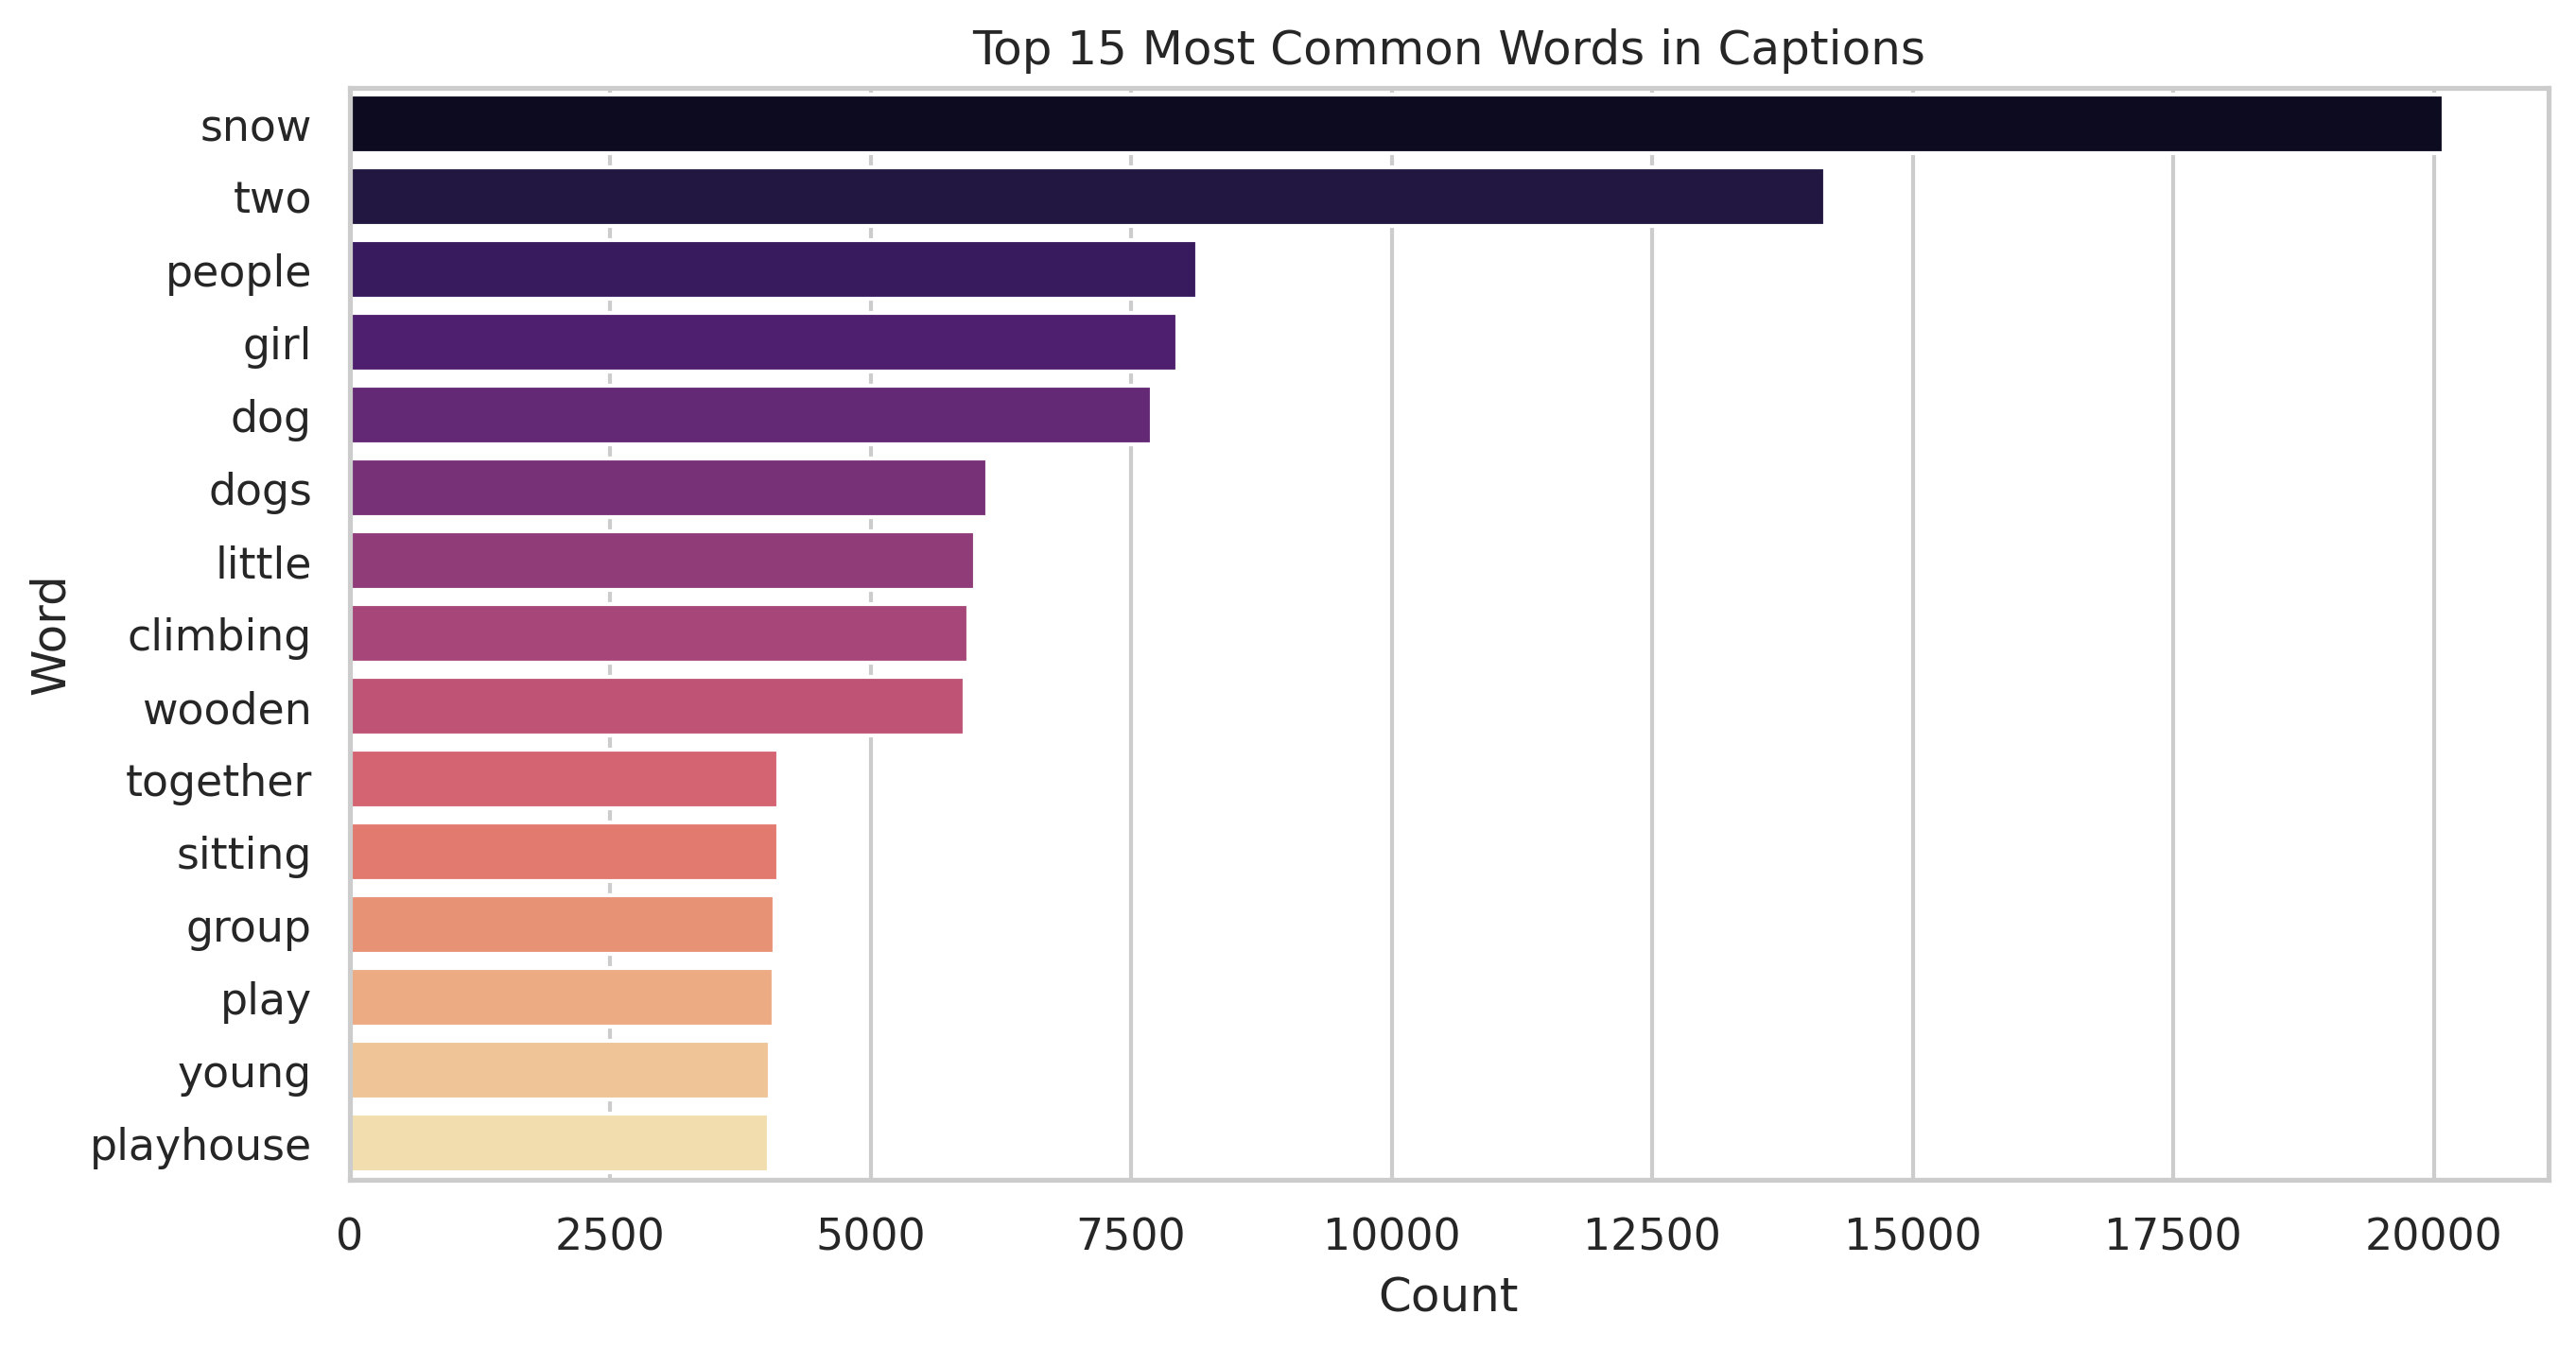
\includegraphics[width=0.80\textwidth]{images/multi_top_words.png}
    \caption{\textbf{Figure MM-5} --- Top 20 Caption Words after Stopword Removal. Generated by \texttt{Counter} on all tokenised captions with a standard English stopword list applied.}
    \label{fig:multi_words}
\end{figure}

\begin{itemize}
    \item \textbf{Subject nouns dominate:} \textit{dog}, \textit{man}, \textit{woman}, \textit{boy}, \textit{child}, \textit{people} --- Flickr8k is rich in photographs of people and animals.
    \item \textbf{Action verbs are frequent:} \textit{running}, \textit{playing}, \textit{standing}, \textit{walking} --- the captions describe dynamic, real-world activities.
    \item \textbf{Colour and material descriptors:} \textit{white}, \textit{black}, \textit{red}, \textit{water} --- spatial and visual context is consistently described.
    \item \textbf{No abstract vocabulary:} The text is grounded exclusively in observable, tangible scenes --- ideal for cross-modal alignment.
\end{itemize}

\subsubsection*{Word Count vs.\ Character Count in Captions}

Figure MM-6 below plots word count against character count for all captions, confirming the very tight, well-controlled nature of the annotation process:

\begin{figure}[H]
    \centering
    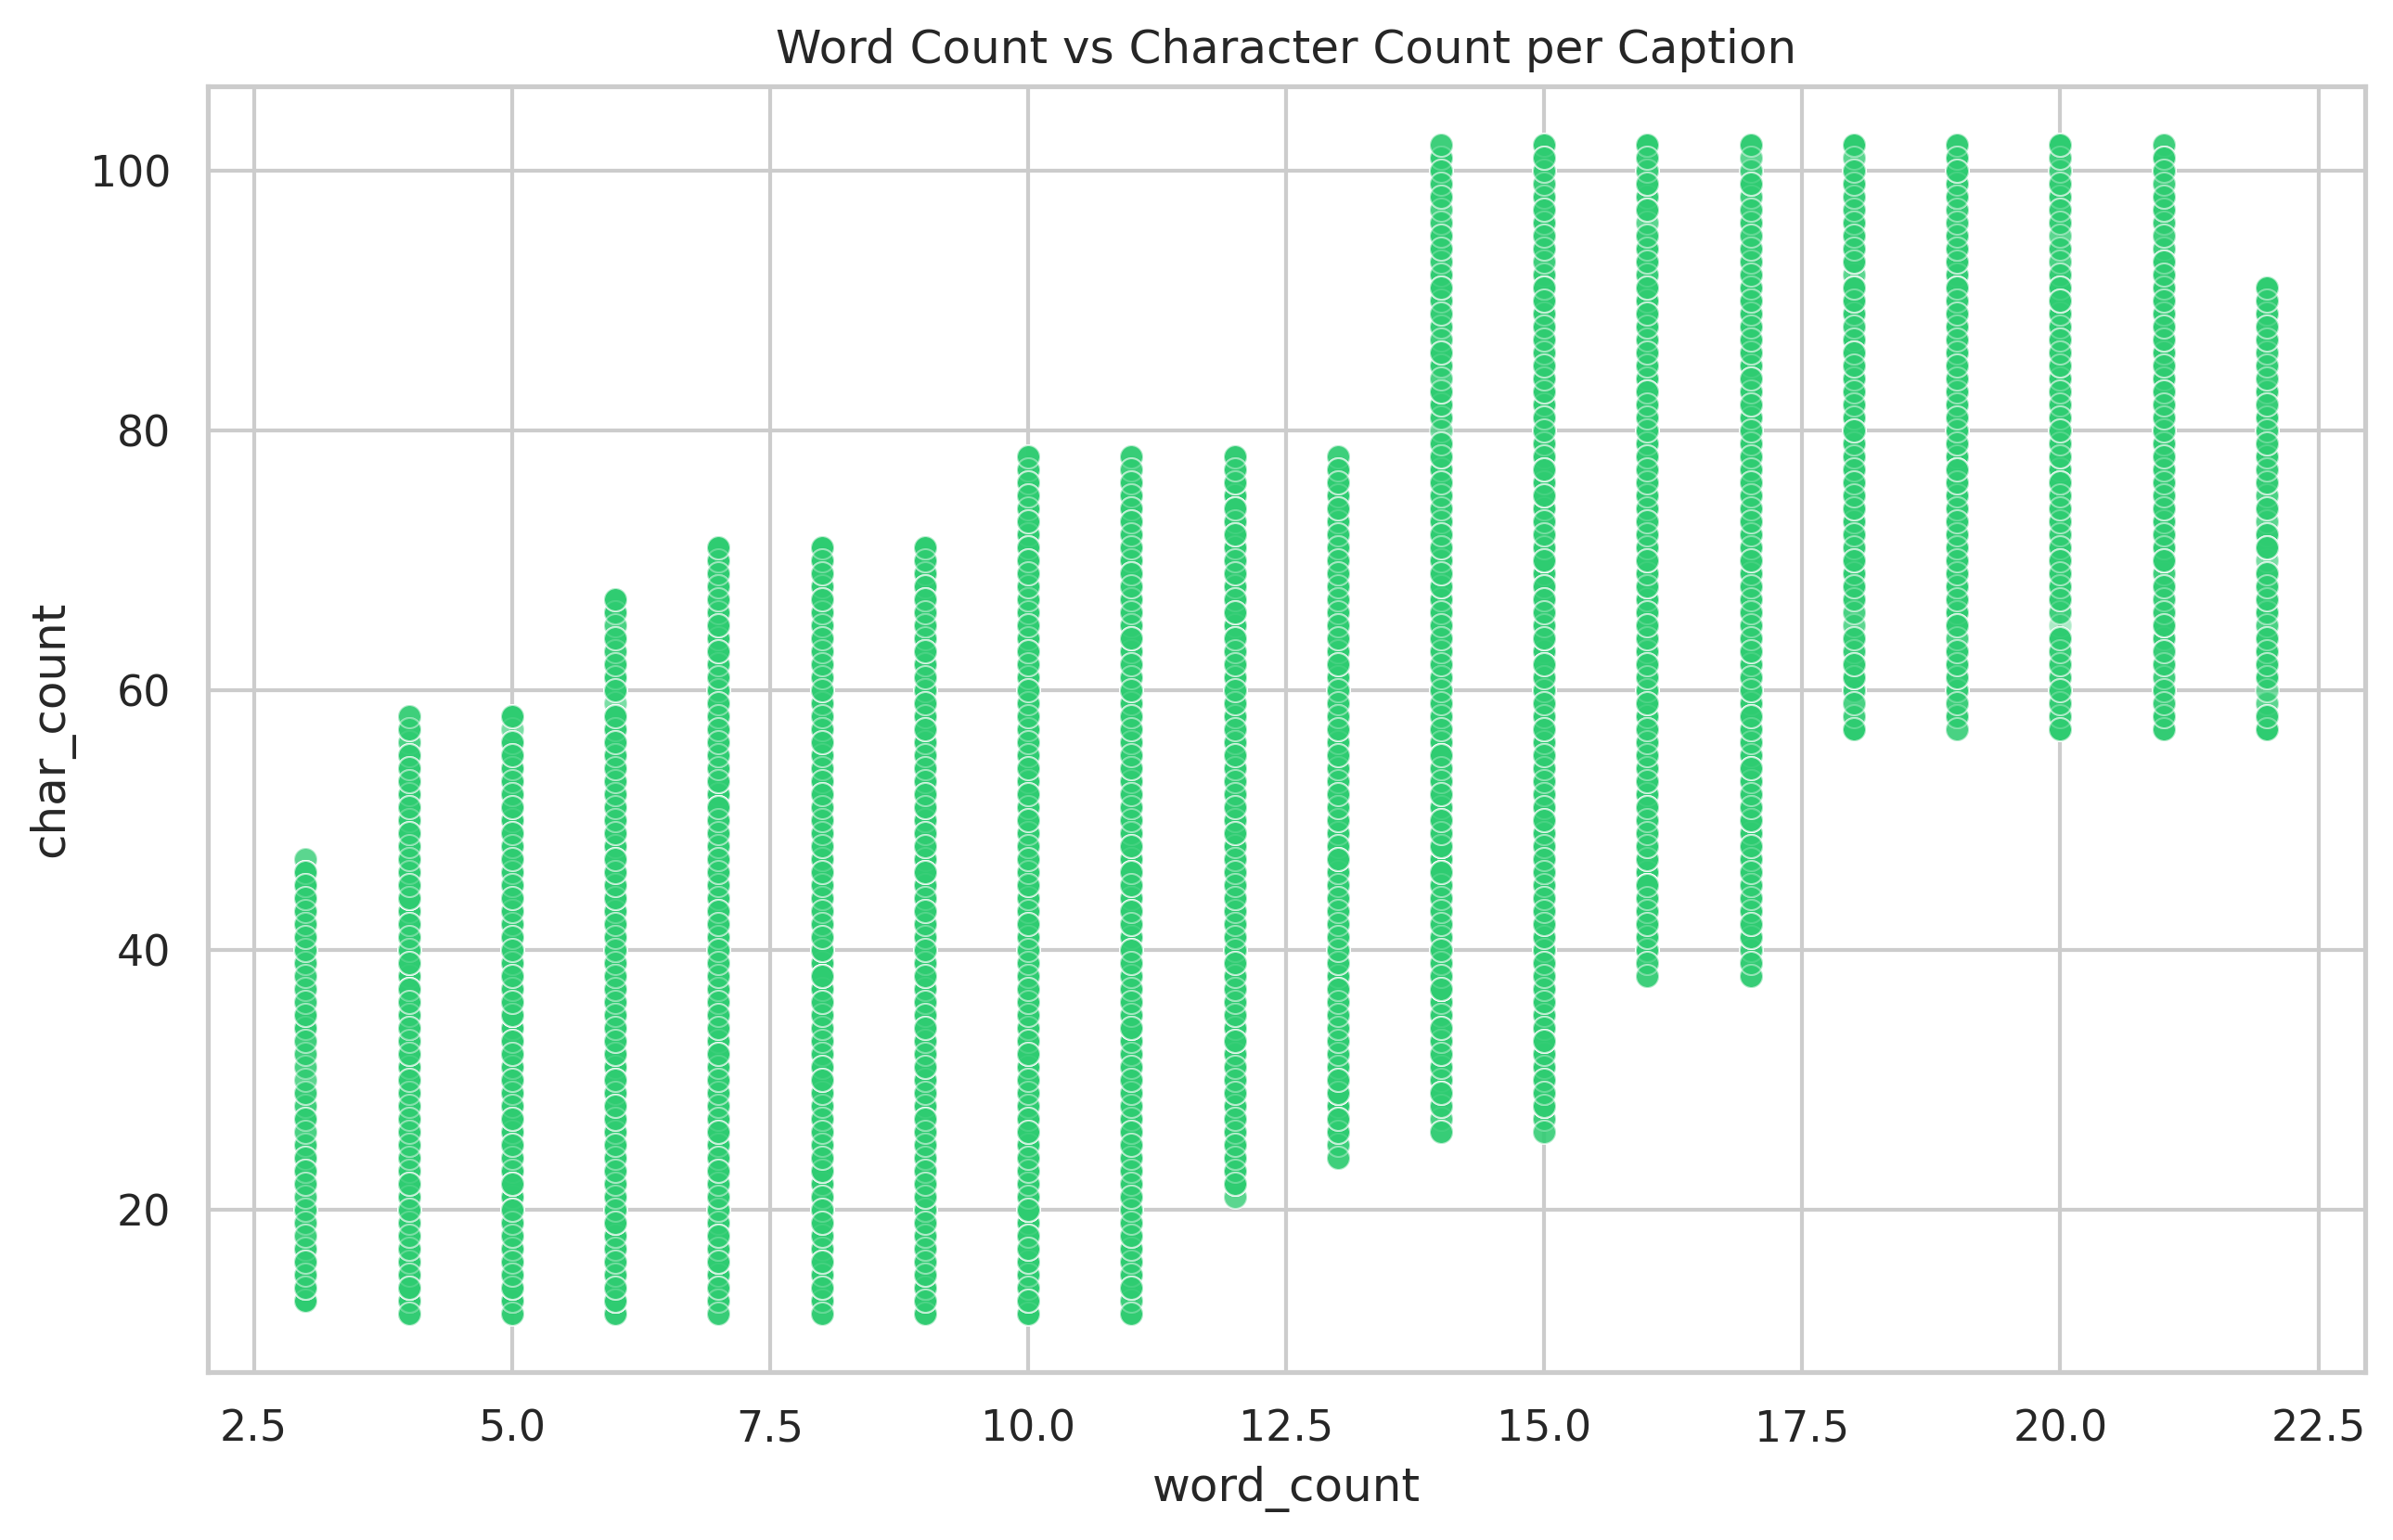
\includegraphics[width=0.75\textwidth]{images/multi_word_char.png}
    \caption{\textbf{Figure MM-6} --- Word Count vs.\ Character Count for Flickr8k Captions. The near-linear relationship confirms consistent writing style across all 5 annotators per image.
    \textit{Code:} \texttt{plt.scatter(df['n\_words'], df['cap\_len'])}.}
    \label{fig:multi_word_char}
\end{figure}

The tight, near-linear scatter (no outlier clouds) confirms that all 5 annotators per image maintained a \textbf{consistent linguistic register}: short words ($\sim$4--6 chars each on average), standard sentence structure, and no extreme verbosity. This homogeneity is beneficial for model training --- the caption space is predictable and bounded.

\subsection{Key Findings and Preprocessing Recommendations}

\begin{importantbox}
\textbf{Summary of Multimodal EDA Key Findings:}
\begin{itemize}
    \item \textbf{Dual-modality structure:} 8{,}092 images $\times$ 5 captions each = 40{,}460 caption-image pairs. Perfect 1:5 alignment, zero missing data. High data integrity confirmed.
    \item \textbf{Non-uniform image resolution:} Images range widely in size (most longest-edge = 500 px). Uniform spatial preprocessing is mandatory before any CNN or ViT backbone.
    \item \textbf{Richer pixel diversity than CIFAR-10:} RGB distributions are broader and multi-modal, reflecting real-world photographic diversity. Use ImageNet normalisation constants when using pre-trained encoders.
    \item \textbf{Short, consistent captions:} 90\% of captions are 8--15 words. \texttt{max\_length = 25} tokens provides $\sim$97\% coverage with minimal padding waste.
    \item \textbf{Human-centric vocabulary:} Dominant content words (\textit{dog, man, woman, boy, running, playing}) reflect the dataset's bias toward people and animals in outdoor, dynamic settings.
    \item \textbf{Recommended preprocessing pipeline:}
    \begin{enumerate}
        \item \textbf{Images}: Resize with aspect-ratio-preserving padding $\rightarrow$ $224\times224$ crop $\rightarrow$ normalize with ImageNet mean/std.
        \item \textbf{Captions}: Lowercase $\rightarrow$ tokenise (BPE or word-level) $\rightarrow$ add \texttt{[BOS]} / \texttt{[EOS]} tokens $\rightarrow$ pad/truncate at \texttt{max\_length=25}.
        \item \textbf{Alignment}: Build an index mapping each image to its 5 captions; during training, randomly sample 1 caption per image per epoch for data augmentation.
    \end{enumerate}
    \item \textbf{Recommended models:} \textbf{CLIP} (OpenAI) for zero-shot cross-modal retrieval; \textbf{BLIP} or \textbf{GIT} for fine-tuned image captioning on this dataset.
\end{itemize}
\end{importantbox}

% =========================================================
% PROJECT LINKS SECTION
% =========================================================
\newpage
\section*{Project Links \& Resources}
\addcontentsline{toc}{section}{Project Links \& Resources}

This report is accompanied by a fully interactive web-based EDA Report, open-source code, and a presentation video. Please visit the following links for full details:

\begin{itemize}
    \item \textbf{Interactive Landing Page:} \url{https://dangkhoi-dev.github.io/P4AI-DS/}
    \item \textbf{Source Code Repository:} \url{https://github.com/dangkhoi-dev/P4AI-DS}
    \item \textbf{Presentation Video (YouTube):} \url{https://youtu.be/A8Z70vnC_fE}
\end{itemize}

% =========================================================
% ATTRIBUTION & DATA SOURCES SECTION
% =========================================================
\section{Attribution \& Data Sources}

In compliance with data usage policies and academic integrity, we would like to acknowledge the original authors, creators, and curators of the datasets used in this Exploratory Data Analysis report. The datasets were sourced from the following repositories:

\begin{itemize}
    \item \textbf{Titanic Dataset (Tabular Data):} \\
    Sourced from Kaggle. This dataset provides passenger information and survival status from the Titanic disaster. \\
    \textbf{Link:} \url{https://www.kaggle.com/datasets/yasserh/titanic-dataset}

    \item \textbf{SMS Spam Collection (Text Data):} \\
    Sourced from Kaggle. A public set of SMS labeled messages that have been collected for mobile phone spam research. \\
    \textbf{Link:} \url{https://www.kaggle.com/datasets/marslinoedward/sms-spam-dataset/data}

    \item \textbf{CIFAR-10 Dataset (Image Data):} \\
    Collected by Alex Krizhevsky, Vinod Nair, and Geoffrey Hinton. The dataset consists of 60,000 32x32 color images in 10 classes. \\
    \textbf{Link:} \url{https://www.cs.toronto.edu/~kriz/cifar.html}

    \item \textbf{Flickr8k Dataset (Multimodal Data):} \\
    Sourced from Kaggle. A standard benchmark dataset containing 8,000 images, each paired with 5 different human-annotated captions. \\
    \textbf{Link:} \url{https://www.kaggle.com/datasets/adityajn105/flickr8k}
\end{itemize}

\input{chapters/2}
\input{chapters/3}


\end{document}
